\documentclass[12pt, 8.5x11]{report}

% Adjust the margin's length and line spacing
\usepackage{geometry}
\usepackage{setspace}
\geometry{left=1.5in,right=1.0in,top=1.0in,bottom=1.0in,includefoot}
\doublespacing

% Initally use roman numbering
\pagenumbering{roman}

% Adjust the appearance of the Table of Contents
\usepackage{tocbibind}
\usepackage[titles,subfigure]{tocloft}

% Extra packages
\usepackage[utf8]{inputenc}
\usepackage{subfig}
\usepackage{acronym}
\usepackage{url}
\usepackage[table]{xcolor}
\usepackage{cite}
\usepackage[pdftex]{graphicx}
\usepackage{pifont}
\usepackage{tikz}
\usetikzlibrary{positioning}
\usepackage{pgfplots}
\usepackage{moreverb}
\usepackage{listings}
\usepackage[chapter]{algorithm}

% Handle abbreviations
\newcommand*{\glossaryname}{Abbreviations}
\usepackage[nonumberlist,toc]{glossaries}
\newacronym{oss}{OSS}{Open Source Software}
\newacronym{vcs}{VCS}{Version Control System}
\newacronym{vcm}{VCM}{Version Control Management}
\newacronym{dvcs}{DVCS}{Distributed Version Control System}
\newacronym{svn}{SVN}{Apache Subversion}
\newacronym{svm}{SVM}{Support Vector Machine}
\newacronym{api}{API}{Application Programming Interface}
\newacronym{sql}{SQL}{Structured Query Language}
\newacronym{msr}{MSR}{Mining Software Repositories}
\newacronym{ld}{LD}{Levenshtein Distance}
\newacronym{nld}{NLD}{Normalized Levenshtein Distance}
\newacronym{cte}{CTE}{Common Table Expressions}
\newacronym{rf}{RF}{Random Forest}
\newacronym{ann}{ANN}{Artifical Neural Network}
\newacronym{ir}{IR}{Information Retrieval}
\newacronym{swr}{SWR}{Sample Window Range}
\makeglossaries

% thesisTitle(newcommand)
% Creates a thesis title page.
% [1]: Student's name (i.e., Roger Random)
% [2]: Thesis title (i.e., Awesome Thesis Work)
% [3]: Degree type (i.e., Masters of Science)
% [4]: Degree area (i.e., Computer Science)
% [5]: University's name (i.e., University of Ontario Institute of Technology)
% [6]: Supervisor's name(s) (i.e., Dr. Radar Muppet)
% [7]: Completion month (i.e., August)
% [8]: Completion year (i.e., 2012)
%
\newcommand{\thesisTitle}[8]{
  \title{#2}
  \author{#1}

  \begin{titlepage}
    \centering
    {\huge #2}
    \\[1cm]

    by
    \\[1cm]

    {\Large #1}
    \\[2cm]

    \begin{minipage}{3in}
      \centering
      \singlespacing{A thesis submitted in partial fulfillment of the requirements for the degree of}
    \end{minipage}
    \\[0.5cm]

    {\large #3}

    in

    {\large #4}
    \\[1cm]

    {\large #5}
    \\[1.5cm]

    {\large Supervisor: #6}
    \\[1.5cm]

    #7 #8
    \\[0.5cm]

    {Copyright \copyright\ #1, #8}
  \end{titlepage}
}


\usepackage{tabularx}
\usepackage{hyperref}
\usepackage{url}

% \usepackage{graphicx}
% \usepackage{wrapfig}
% \usepackage{lscape}
% \usepackage{rotating}
% \usepackage{epstopdf}

\usepackage{rotating}
\usepackage{pdflscape}
\usepackage{everypage}

% Command for changing the page number position to be placed at the bottem center for landscape
% Note in order to prevent duplcate page numbers, \thispagestyle{empty} should be used.
\newlength{\hfoot}
\newlength{\vfoot}
\AddEverypageHook{\ifdim\textwidth=\linewidth\relax
\else\setlength{\hfoot}{-\topmargin}%
\addtolength{\hfoot}{-\headheight}%
\addtolength{\hfoot}{-\headsep}%
\addtolength{\hfoot}{-.5\linewidth}%
\ifodd\value{page}\setlength{\vfoot}{\oddsidemargin}%
\else\setlength{\vfoot}{\evensidemargin}\fi%
\addtolength{\vfoot}{\textheight}%
\addtolength{\vfoot}{\footskip}%
\raisebox{\hfoot}[0pt][0pt]{\rlap{\hspace{\vfoot}\rotatebox[origin=cB]{90}{\thepage}}}\fi}

\hypersetup{
    colorlinks,
    citecolor=black,
    filecolor=black,
    linkcolor=black,
    urlcolor=black
}

\begin{document}

\thesisTitle
  {Joseph Heron}
  {Method Level Change Prediction Using Commit History Data}
  {Master of Science}
  {Computer Science}
  {University of Ontario Institute of Technology}
  {Dr. Jeremy Bradbury}
  {April}
  {2016}

\chapter*{Abstract}
\addcontentsline{toc}{chapter}{Abstract}

% Elevator pitch:
Software development and software maintenance require a large amount of source code changes to be made to a software repositories. Any change to a repository can introduce new resource needs which will cost more time and money to the repository owners. Therefore it is useful to predict future code changes in an effort to help determine and allocate resources. We are proposing a technique that will predict whether elements within a repository will change in the near future given the development history of the repository. The development history is collected from source code management tools such as GitHub and stored local in a PostgreSQL. The predictions are developed using the machine learning approaches Support Vector Machine and Random Forest. Furthermore, we will investigate what factors have the most impact on the performance of predicting using either Support Vector Machines or Random Forest with future code changes using commit history. Visualizations were used as part of the approach to gain a deeper understanding of each repository prior to making predictions. To validate the results we analyzed open source Java software repositories including; acra, storm, fresco, dagger, and deeplearning4j.

% TODO integrate results from experiments.
\chapter*{Acknowledgments}
\addcontentsline{toc}{chapter}{Acknowledgments}

I would first like to thank my thesis advisor Dr. Bradbury of the Computer Science Faculty at the University of Ontario Institute of Technology. Dr. Bradbury was always available to provide direction and feedback about both research and writing.

I would also like to thank the Dr. Szlichta for his thoughtful advice and recommendations throughout the work on this thesis.

To my colleagues at the University of Ontario Institute of Technology and lab mates in the Software Quality Research Lab, thank you for the stimulating discussions throughout the last two years.

Finally, I must express my very profound gratitude to my family and friends for providing me with unfailing support and continuous encouragement throughout my years of study, research and writing. This accomplishment would not have been possible without them. Thank you.

% Include lists in singlespacing
\singlespacing
\tableofcontents
\listoffigures
\listoftables
\lstlistoflistings
\printglossary[style=list]
\clearpage
\doublespacing

\pagenumbering{arabic}

% Include the Chapters
\chapter{Introduction}
\label{chap:introduction}

Introduction here with example \gls{api} and citation~\cite{Ran12}

%\chapter{Background}
\label{chap:background}


\section{Mining Open Source Software Repositories}

% TODO ensure this is accurate.
\gls{oss} generally is software that provides with the ability access the source code and make modifications to the source code. While certain licenses provide some restrictions on the ability to redistribute the software the main point of the source code of the software being freely available is key. The scope and capability of \gls{oss} projects vary greatly. Several very popular \gls{oss} projects are listed in table \ref{tab:oss_projects}.

%TODO make sure footnotes fit in better.
\begin{table}[h!]
\begin{minipage}{\textwidth}
\begin{center}
    \begin{tabular}{|l|l|l|}
        \hline
        Owner & Project & Description \\
        \hline

        Mozilla & Firefox\footnote{\url{https://www.mozilla.org/en-US/firefox/desktop/}} & Internet Browser \\
        Linux & Linux Kernel\footnote{\url{https://www.kernel.org/}} & Operation System Kernel \\
        VideoLAN & VLC\footnote{\url{http://www.videolan.org/vlc/index.html}} & Media Player \\
        PostgreSQL & PostgreSQL\footnote{\url{http://www.postgresql.org/}} & Object-Relational Database Management System \\
        git & git\footnote{\url{https://git-scm.com/}} & Version Control System \\
        \hline
    \end{tabular}
\end{center}
\caption{Open Source Software Projects}
\label{tab:oss_projects}
\end{minipage}
\end{table}
%Firefox => MPL 2.0
%Linux Kernel => GPL v2, plus various closed-source binary blobs
%VLC => GPLv2+ (player), LGPLv2.1+ (engine)
%PostgreSQL => PostgreSQL License
%git => GNU General Public License v2, GNU Lesser General Public License 2.1

The development of large software projects (whether \gls{oss} or not) often make use of \gls{vcs}. A \gls{vcs} helps the developers of the project manage the changes of the project and facilitate the collaboration between developers. A \gls{vcs} will keep an current version of the project and keep track of the previous version of the project as well. This may be done through keeping a copy of each version of the project or by keeping track of all each change made to the project. \gls{svn} and git would be two examples of \gls{vcs}s.

Git is a \gls{dvcs} and differs greatly from \gls{svn} which is a normal \gls{vcs}. Git will provide the user with a complete copy of the repository that is worked on independent of network connection. The independence of each repository also allows for a repository to be developed without a centralized server. The distributed aspect of git tends to allows for easier use for all involved parities. The one main issue with a \gls{dvcs} is that while decentralization is useful, developers will require some method to collaborate and communicate to transfer changes made to the repository. Therefore typically one centralized server is used to maintain communication between all interested parties.

Git has grown in popularity since it was created and is at the core of several \gls{vcm} sites such as GitHub \footnote{\url{https://github.com/}}, BitBucket \footnote{\url{https://bitbucket.org/}} and GitLab \footnote{\url{https://gitlab.com/}}. These platforms tend to be fairly supportive of \gls{oss} projects through providing their services free of charge. For example, GitHub provides unlimited public repositories completely free. While these projects do not have to be licensed with an open source license typically they will be since they are already publicly visible.

% GitLab -> https://gitlab.com/
% GitHub -> https://github.com/
% BitBucket -> https://bitbucket.org/

GitHub is the most popular of the \gls{vcm} websites and hosts numerous very popular \gls{oss} projects including, the Linus Kernel, Swift\footnote{\url{https://swift.org/}} and React\footnote{\url{https://facebook.github.io/react/}}. GitHub also provides a public \gls{api} to allow for access to the data related to project repositories which is discussed further below. % TODO link to that.
Given the popularity of GitHub for use by developers and the availability of the project data, GitHub is an obvious choice for mining project data. Especially since the goal of mining software is to capture \gls{oss} project data to both explore and test analysis methods. Publicly visible projects are also publicly accessible through the \gls{api} and the majority are open source.

%%%%%%%%%%

Git provides a simple interface to manage the repository regardless of which site is the central server. Therefore regardless which site the project resides on users can easily interact with the project as long as they know the git interface. Git in essences is a file storage for the project that keeps track of changes made to the project. A \textit{commit} is a set of changes that a developer has made at a certain time. The developer has full control what gets committed, when it gets committed and even modified at a later date.
%This results in the date of the commit merely identifying when the developer formally notified Git that a change was made.

A branch is a series of commits that are often related. In figure \ref{fig:network_diagram}, each dot would represent a commit and a set of dots connected by the same colored lines are a branch. Branches can be considered different paths or deviations in the development from each other allowing for different versions of the project to be maintained and developed. The \textit{master} branch is the main branch, represented with black, from which all branches usually stem from and is generally where projects are developed on. On a similar note, a \textit{tag} is a branch that is frozen to allow for future reference. Tags are often uses to mark a significant point in the development history such as a project release. Finally, when two differently branches converge into a single dot then the two branches have been \textit{merged}. A merge indicates that the differences between the two branches are consolidated based on the developer's discretion.

\begin{figure}[!ht]
    \centering
        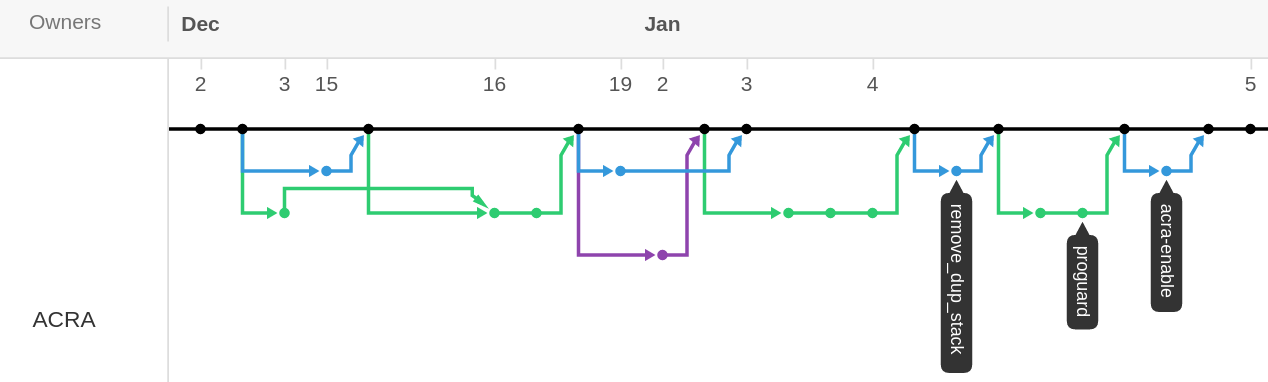
\includegraphics[width=1.0\textwidth]{images/network}
    \caption{Network diagrams}
    \label{fig:network_diagram}
\end{figure}

A commit consists of files that have been changed, more specifically a list of \textit{patch} files which each outline the changes made to their corresponding file. The patch file consists of a series of differences between the previous version of the file and this new version of the file. These patch files are key since they contain the actual changes made to the project and thus are the major point of interest.

% TODO fix close

\section{Machine Learning}

% Rase, realizing software engineering learning
Machine learning is a complex method for software algorithms to attempt to determine patterns within the data. One such problem example would be an algorithm to detect certain people within an image. For an individual such a task may seem trivial however for a software system to detect it is far more difficult. Algorithms that can determine patterns and mimic them from abstract set of data is useful when such patterns are extremely complex. A few examples of such algorithms are \gls{svm}, ...


\section{Change Prediction}

% Related work stuff here or later

The development of large scale projects can take a long time and involve a huge time investment from the developers. The development of the project will cause for the developers to make changes to projects. Software projects will have faults within the project especially during the development phase. A project in its early stages may not meet the full set of functionality since it has not been completed yet. Since the development team will known that such features are not yet implemented these faults or fails are not a huge concern. Rather faults that are unknown to the developer team are far more serious. Such cases as a feature was thought to be implemented correct but was not or a feature implementation breaks other features. In both those cases changes made to the project cause the fault to be revealed.

Changes to the project are the means by which all development occurs. The ability to analyze and predict changes within a project could give deep insights into the development of a project. 

% TODO talk about previous work on change prediction. cause. 
\chapter{Literature Review}
\label{chap:related_works}


\section{Data Mining}

Data collection from some original source provides access to a data set that may not be initially available. This data source could also be in a state that is not convenient or feasible for use without leveraging data mining techniques to transform the data to a more accessible state. The source of the data can vary greatly based on the interests for the individual(s) collecting the data. Data mining has mostly focused on single source mining and multiple data sources. Data mining in general has however also taken a large focus on data collection from software repositories which can be either single or multiple source \cite{Hemmati2013}, \cite{Hassan2006}, ... %TODO list other msr based papers.
% TODO find other work of data mining

% MSR, guiding future changes
Zimmermann et al. map the changes that certain developers make and who change certain functions to the functions they also change \cite{Zimmermann2005a}. 

% Change analysis
Maletic and Collard investigate changes with a software project's development cycle. The changes are extracted and stored in an more easily usable representation \cite{Maletic2004}.

% MSR Change extraction of changes
Canfora et al. propose a method for extracting and refining the changes made throughout the life a project to be used in more effective analyses \cite{Canfora2007c}.

Hemmati et al. take a comprehensive look at the research related to \gls{msr} to determine best practices and point towards future work \cite{Hemmati2013}.

% MSR in general
Hassan cover the different metrics and uses of \gls{msr} \cite{Hassan2006}.

% Validation of Change history research, benchmark
Dit et al. provide a benchmark dataset to help in the testing and comparing of various methods for improving software maintenance tasks \cite{Dit2013}.

% TODO MERGE this with related work
\subsection{Mining Open Source Software Repositories}

% TODO ensure this is accurate.
\gls{oss} generally is software that provides with the ability access the source code and make modifications to the source code. While certain licenses provide some restrictions on the ability to redistribute the software the main point of the source code of the software being freely available is key. The scope and capability of \gls{oss} projects vary greatly. Several very popular \gls{oss} projects are listed in table \ref{tab:oss_projects}.

%TODO make sure footnotes fit in better.
\begin{table}[h!]
\begin{minipage}{\textwidth}
\begin{center}
    \begin{tabular}{|l|l|l|}
        \hline
        Owner & Project & Description \\
        \hline
        Mozilla & Firefox\footnote{\url{https://www.mozilla.org/en-US/firefox/desktop/}} & Internet Browser \\
        Linux & Linux Kernel\footnote{\url{https://www.kernel.org/}} & Operation System Kernel \\
        VideoLAN & VLC\footnote{\url{http://www.videolan.org/vlc/index.html}} & Media Player \\
        PostgreSQL & PostgreSQL\footnote{\url{http://www.postgresql.org/}} & Object-Relational Database Management System \\
        git & git\footnote{\url{https://git-scm.com/}} & Version Control System \\
        \hline
    \end{tabular}
\end{center}
\caption{Open Source Software Projects}
\label{tab:oss_projects}
\end{minipage}
\end{table}
%Firefox => MPL 2.0
%Linux Kernel => GPL v2, plus various closed-source binary blobs
%VLC => GPLv2+ (player), LGPLv2.1+ (engine)
%PostgreSQL => PostgreSQL License
%git => GNU General Public License v2, GNU Lesser General Public License 2.1

The development of large software projects (whether \gls{oss} or not) often make use of \gls{vcs}. A \gls{vcs} helps the developers of the project manage the changes of the project and facilitate the collaboration between developers. A \gls{vcs} will keep an current version of the project and keep track of the previous version of the project as well. This may be done through keeping a copy of each version of the project or by keeping track of all each change made to the project. \gls{svn} and git would be two examples of \gls{vcs}s.

Git is a \gls{dvcs} and differs greatly from \gls{svn} which is a normal \gls{vcs}. Git will provide the user with a complete copy of the repository that is worked on independent of network connection. The independence of each repository also allows for a repository to be developed without a centralized server. The distributed aspect of git tends to allows for easier use for all involved parities. The one main issue with a \gls{dvcs} is that while decentralization is useful, developers will require some method to collaborate and communicate to transfer changes made to the repository. Therefore typically one centralized server is used to maintain communication between all interested parties.

Git has grown in popularity since it was created and is at the core of several \gls{vcm} sites such as GitHub \footnote{\url{https://github.com/}}, BitBucket \footnote{\url{https://bitbucket.org/}} and GitLab \footnote{\url{https://gitlab.com/}}. These platforms tend to be fairly supportive of \gls{oss} projects through providing their services free of charge. For example, GitHub provides unlimited public repositories completely free. While these projects do not have to be licensed with an open source license typically they will be since they are already publicly visible.

% GitLab -> https://gitlab.com/
% GitHub -> https://github.com/
% BitBucket -> https://bitbucket.org/

GitHub is the most popular of the \gls{vcm} websites and hosts numerous very popular \gls{oss} projects including, the Linus Kernel, Swift\footnote{\url{https://swift.org/}} and React\footnote{\url{https://facebook.github.io/react/}}. GitHub also provides a public \gls{api} to allow for access to the data related to project repositories which is discussed further below. % TODO link to that.
Given the popularity of GitHub for use by developers and the availability of the project data, GitHub is an obvious choice for mining project data. Especially since the goal of mining software is to capture \gls{oss} project data to both explore and test analysis methods. Publicly visible projects are also publicly accessible through the \gls{api} and the majority are open source.

%%%%%%%%%%

Git provides a simple interface to manage the repository regardless of which site is the central server. Therefore regardless which site the project resides on users can easily interact with the project as long as they know the git interface. Git in essences is a file storage for the project that keeps track of changes made to the project. A \textit{commit} is a set of changes that a developer has made at a certain time. The developer has full control what gets committed, when it gets committed and even modified at a later date.
%This results in the date of the commit merely identifying when the developer formally notified Git that a change was made.

A branch is a series of commits that are often related. In figure \ref{fig:network_diagram}, each dot would represent a commit and a set of dots connected by the same colored lines are a branch. Branches can be considered different paths or deviations in the development from each other allowing for different versions of the project to be maintained and developed. The \textit{master} branch is the main branch, represented with black, from which all branches usually stem from and is generally where projects are developed on. On a similar note, a \textit{tag} is a branch that is frozen to allow for future reference. Tags are often uses to mark a significant point in the development history such as a project release. Finally, when two differently branches converge into a single dot then the two branches have been \textit{merged}. A merge indicates that the differences between the two branches are consolidated based on the developer's discretion.

\begin{figure}[!ht]
    \centering
        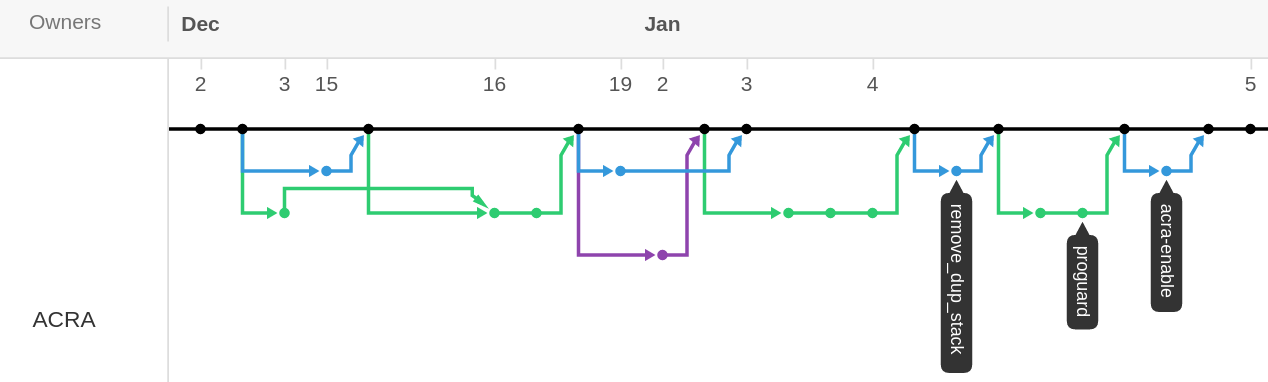
\includegraphics[width=1.0\textwidth]{images/network}
    \caption{Network diagrams}
    \label{fig:network_diagram}
\end{figure}

A commit consists of files that have been changed, more specifically a list of \textit{patch} files which each outline the changes made to their corresponding file. The patch file consists of a series of differences between the previous version of the file and this new version of the file. These patch files are key since they contain the actual changes made to the project and thus are the major point of interest.

% TODO fix close

\section{Machine Learning}

% Rase, realizing software engineering learning
Machine learning is a complex method for software algorithms to attempt to determine patterns within the data. One such problem example would be an algorithm to detect certain people within an image. For an individual such a task may seem trivial however for a software system to detect it is far more difficult. Algorithms that can determine patterns and mimic them from abstract set of data is useful when such patterns are extremely complex. There are numerous algorithms which apply machine learning approaches. Each approach has both advantages or disadvantages. Some examples of machine learning algorithms are \gls{svm}, \gls{rf} and \gls{ann}. The three provided examples are also commonly used for data mining \cite{Alam2013}, \cite{Granitto2007}, \cite{Westland2011}, \cite{Yu2011}, \cite{Huang2007}, \cite{Jalbert2012} %TODO get some papers for svm and ann

Bhattacharyya et al. provide a detailed description of \gls{rf} and \gls{svm}.

\subsection{Support Vector Machines}
\label{subsec:svm_prediction}

\gls{svm} models are more easily modified to fit data from different sources since they flexible and robust than more classical linear regression models *cite*. %TODO consider citing 

A \gls{svm} is used to predict what type of change will occur based on a set of features provided. A feature is a data extracted from the project represented as a floating point number. In order to be useful a feature must in some way characterize the the category that it is assigned to. The feature must also not rely on the category that it belongs to in order to be calculated. For example, given a category of the method change within the next 5 commits or not, then the features must not rely on knowledge of future changes to the project. If the features fail to effectively characterize the category they are assigned to then the \gls{svm} may have poor predictions. It is also necessary for the features to independent of each other to not negatively affect the categorization.


\gls{svm} has been widely used for making predictions for various aspects including predicting battery charge state \cite{Anton2013}, pharmaceutical data \cite{Burbidge2001}, software faults \cite{Gondra2008, Erturk2015, Malhotra2015, Kim2008, Moeyersoms2015, Neuhaus2007}, bug localization \cite{Murphy2007, Neuhaus2007}, software mutation testing score \cite{Jalbert2012}, financial stocks \cite{Kim2003}, credit score \cite{Huang2007}, credit card fraud \cite{Westland2011}, solar power output \cite{Zeng2016}.

Malhotra reviews numerous machine learning techniques, including \gls{svm} and \gls{rf}, used by various studies. The results of which outline where each approaches succeed and falls short. When using a machine learning algorithm it is imperative to use a suitable algorithm for current situation. Kim et al. outline a approach that uses a \gls{svm} to predict changes that will occur within the project. By identifying these changes the a project developer can potentially locate a bug within a change and fix it prior to being reported. Erturk and Sezer compare the performance of their proposed method, an Adaptive Neuro Fuzzy Inference System, to that of an \gls{svm} for predicting software faults. The models are trained using project metrics as well as the project's historical fault data. Zeng and Qiao use a \gls{svm} to provide short-term predict solar power output. The \gls{svm} model outperformed both an autoregressive and a neural network model. Anton et al. propose a method for predicting the state of charge of a battery using \gls{svm} model.

Bhattacharyya et al. uses \gls{rf}, \gls{svm}, logistic regression to detect credit card fraud. Both \gls{rf} and \gls{svm} are able to predict a large number of fraudulent credit card transactions.


% TODO talk even more about how to pick better features.
%<<< TODO Example feature vector >>>

% \begin{table}
% \begin{center}
%     \begin{tabular}{|l l l l l l l|l|}
%         \hline
        
%         Features &  &  &  &  &  &  & Description \\
%         \hline
%         $name$ & $signature$ & $change_i$ & $committer$ & $freq_{change}$ & $change_{prev}$ & $t_\Delta$ & $change_{next\_6}$ \\
%         %0.0 & 0.1 & 0.0\\
%         \hline
%     \end{tabular}
% \end{center}
% \caption{Example Feature Vector}
% \label{tab:example_feature_vector}
% \end{table}

% TODO Format parts of this.
\gls{svm} requires all feature data be encoded as floating point numbers. For any numerical data the conversion to floating point is trivial. However, for more complex data the conversion is a little more difficult. Categorical data can be mapped into a unique vector entry per category. For example, if a feature can be 1 of 3 options: 0, 1 or 2 then it can be converted into three entries in the feature vector. Encoding the value 2 the sub-vector of the feature set would be [0, 0, 1] where 1 indicates a field that feature is present in the data for this vector, and 0 indicates the feature is not present. Data that is in the form of a string can be converted to a floating point number by assigning a unique number for each string (similar to hashing). The one downside to this method is that the numbers corresponding to each string maintain no numerical properties. In essence the data becomes categorical, such that if \textit{bob} is mapped to 1 and \textit{sally} is mapped to 2 there is no relationship between 1 and 2. Ideally, this data would then be further converted using the previously described method however if the set of possible strings is large then it may be unreasonable to convert it. For example, if there are 100 possible strings then that would add 100 new entries to a single vector.

%<<< TODO svm diagrams >>>

The categorization is used for the prediction, where each value of the category relates to a unique prediction type. For example, a simple binary categorization could simply 1 or 0 where 1 predicts the event will occur and 0 predicts that the event will not occur. In essence an \gls{svm} is tasked with separating a dataset into two different categories given a sample set of data that has already been categorized into two subsets. Given the categorization of the sample dataset the \gls{svm} model is trained to allow for categorization of new data. The categorization of any new vectors (that were not used for training) is called a prediction and is made by the \gls{svm} model created through the training. More specifically, the sample dataset is a dataset extracted from the target dataset. The sample dataset is then categorized based on the predetermined criteria (the prediction goal). This dataset along with the categorization for each vector in the dataset is the training dataset, and is then used to \textit{train} the \gls{svm} model. Once the model has been trained, the \gls{svm} model is ready to be used for making classification predictions. The data for each feature can be extracted from the new dataset, allowing for the model to classify each new vector. Given that the \gls{svm} model is accurate and reliable the results can then be used towards making predictions about the dataset. For example if the classification is that of predicting change to occur within the next six commits the developer may wish to be careful with the use of the method or assess the method's quality and determine if any issues within the method need to be addressed.

A lower prediction score often relates to the data from the feature set poorly characterizing the categories. Similarly a warning will be given if the dataset is in-separate. In this case, the dataset for each category may be too similar and cannot be properly split into the two category subsets. In both cases a change to the feature set may help, whether that is a decrease or increase of features in the set. Some features are detrimental to the model, especially two features related to one another. Other potential steps would be to modify the data to ...
% *** TODO determine best practices for data something like mean of 1 and std of 1. ***

More details about the specific features used will be given a little later on. Features are descriptive aspects of the dataset that are classified into the predetermined categories. Since these features relate directly to the category understanding of the classification critical and can help determine which features should be used. For example for a classification of whether a change will occur within the next few commits, a useful feature may be the frequency by which a method changes within the project. Picking a descriptive feature set is paramount to providing a strong prediction of future data.

%<<< TODO create a figure to outline the various features and their meaning >>>

Most of this was done using database queries or user defined functions created in the database language.

% TODO get some papers related to support vector machines.

\subsection{Random Forests}
\label{subsec:random_forest_predictions}

\gls{rf} are a popular machine learning algorithm and is used in numerous areas including predictions for software fault \cite{Malhotra2015, Moeyersoms2015, Guo2004}, software development effort \cite{Moeyersoms2015}, credit card fraud \cite{Westland2011}, database indexing \cite{Yu2011}, malware detection \cite{Alam2013}. 

Malhotra provides an extensive review of studies involving machine learning to predict software faults. The results showed that \gls{rf} tended to preform better than other machine learning algorithms studied. Moeyersoms et al. made use of \gls{rf} and \gls{svm} as well as a few other data mining approaches to predict software faults and effort estimation. The data mining techniques are used as part of another model, ALPA rule extraction, to improve the predictions and increase traceability. Guo et al. attempt use \gls{rf} to predict the fault proneness of modules within a project. The \gls{rf} prediction results for the five sample projects prove more accurate to that of a logistic regression. Yu et al. attempt to use \gls{rf} to determine a more effective database indexing for video data. The database index are used to provide faster searching of the database for action detection.

\gls{rf}s are commonly used to on data that has been mined from some source to make predictions \cite{Alam2013}, \cite{Granitto2007}, \cite{Yu2011}. A \gls{rf} leverages numerous decision trees to provide attempt to improve prediction capabilities. Therefore to fully understand a \gls{rf} first an understanding of decision trees is necessary. A decision tree is a technique which will create a tree based on a data set that has been classified. Once the decision tree model is created it can be used to predict or categorize data that has not yet to be classified. In the tree model the leafs will be categorizations where as the connections between inner nodes are the decisions by which the categorizations are made.

% TODO format
One issue with decisions trees and more generally machine learning techniques in general is imbalanced data sets for training the model \cite{Khoshgoftaar2007}. The data set used rarely provided even sample sizes of each set therefore without taking necessary pro-cautions the algorithm will bias the results. In the worse case the model will classify any input data as the larger data classification.

In case of imbalanced datasets there are several methods to help provide stronger predictions \cite{Khoshgoftaar2007}. The most obvious and easiest to attempt would be to sample more data. However if the dataset in general follows this trend then some more advanced techniques can used to improve the model.

% Note when remarking about model quality this refers to accuracy and recall of the model
 
The first method would be to \textit{undersample} larger category this will even out both of the categories. This will remove some of the input values within the dataset to reduce the set size. However if there are very few samples of the smaller category the performance will suffer as well. A second method of \textit{oversampling} is useful in the case were the data samples are small. The input data from the smaller category is selected to be duplicated in the set to increase the size of the set. This helpful since it will increase the size of the dataset but could lead to bias based on the data selected from the smaller dataset. The selection method for which input vectors to over or under sample can be based off on the data's statistical distribution or made by random choice. Another advantage of these over and under sampling is that they can also be used together to in the case of a large disparity between the category's set size. 

% Bootstrapping aggregation
Another feature of \gls{rf} which is used to help provide more reliable predictions is \textit{Bootstrap Aggregation} \cite{Westland2011}. Similar to normal sampling methods it will take the initial dataset. However rather than using the dataset as is the dataset will be uniformly sampled $n$ times and repeated $m$ times to create $m$ datasets of $n$ values. These newly created datasets will then be used to train $m$ models. Finally, when attempting to categorize a new input data it will be given to every model and the prediction result will be aggregated to provide a more accurate results. For some machine learning methods such as \gls{svm} this method will improve the results and help with imbalanced datasets.

A \gls{rf} is a collection of decisions trees trained on random samples of the initial dataset. So the \gls{rf} will take an input dataset and then train $m$ decisions trees using $m$ randomly sampled sub-datasets of the initial dataset. This helps improve the model created and makes \gls{rf}s far easier to use. As well \gls{rf}s have a feature that determines the importance of each feature is assessed during the training of the model \cite{Westland2011}. The importance outlines the quality of each feature in providing the prediction \cite{Verikas2011}. Therefore in order to properly understand the feature importance the accuracy, precision and recall of the model should be determined by running a test dataset to determine the quality of the model.

\section{Software Development Prediction}
% TODO actually write about each of the papers.

%TODO work this together 
Software development prediction contains numerous areas of study which generally attempt to improve projects by focusing on their development and providing feedback to the developers through predictions. Some of these areas include, fault detection \cite{Nagappan2007, Moser2008, Thwin2005, Sisman2012}, mutation score \cite{Jalbert2012}. While there may be a large overlap in the objective for these studies often they will vary in what is used to make the prediction.

% Close source, prediction
%Nagappan and Ball use the software dependencies and churn metrics to predict the failure of a commercial product post release \cite{Nagappan2007}.

% Defect prediction, change attributes, static attributes
%Change and static code attributes are compared in their capability in predicting defects within a project \cite{Moser2008}.

% predict software quality based on code metrics
%Attempt to predict the number of defects within a given class using a neural network trained on object oriented code metrics \cite{Thwin2005}. Second the amount of changes within a class is predicted again with a neural network using object oriented code metrics \cite{Thwin2005}.

% Prediction of something
%Support development of software predictions is a common research area. Jalbert and Bradbury used static metrics from both the source code and corresponding test suites to predict the mutation score for the test suite \cite{Jalbert2012}.

% Bug localization through prediction, change history, defect history, temporal decay.
%Sisman and Kak leverage defect history and the change history of a project to predict which files will be the cause of bugs in different version of the project \cite{Sisman2012}.

\subsection{Change Prediction}
% Related work stuff here or later

The development of large scale projects can take a long time and involve a huge time investment from the developers. The development of the project will cause for the developers to make changes to projects. Software projects will have faults within the project especially during the development phase. A project in its early stages may not meet the full set of functionality since it has not been completed yet. Since the development team will known that such features are not yet implemented these faults or fails are not a huge concern. Rather faults that are unknown to the developer team are far more serious. Such cases as a feature was thought to be implemented correct but was not or a feature implementation breaks other features. In both those cases changes made to the project cause the fault to be revealed.

Changes to the project are the means by which all development occurs. The ability to analyze and predict changes within a project could give deep insights into the development of a project.


A large amount of research as focused on predictions of changes based on changes \cite{Bantelay2013}, \cite{Chaturvedi2014}, \cite{Giger2012}, \cite{Hassan2004}, \cite{Kagdi2007}, \cite{Ying2004}. 

Ying et al. present a method that predicts which parts of the system will change given a set of changes \cite{Ying2004}. The prediction method leverages the change history.

Kagdi and Maletic also leverage version history changes to perform software change predictions \cite{Kagdi2007}. The actually analysis applied is two fold, through the dependency analysis of the current version and the change analysis of the version history. The data is collected through \gls{msr} which is a popular field of study. 

In a similar work, Hassan and Holt, worked towards predicting change propagation of a given initial change. \cite{Hassan2004} The main question was to determine given a change to an entity (e.g. function or variable) will propagate to changes in other entities. This work is very related since it tests various methods and leverages presents the best one.

Bantelay et al. propose a method that mines the file and method level evolutionary couplings to attempt to predict commits and other interactions within the project \cite{Bantelay2013}. Both methods were used in isolation as well to determine whether the attributes were more helpful when used together.

Giger et al. attempt to build off of previous work in change prediction (proneness) by providing predictions relating to more refined entities \cite{Giger2012}. The syntax changes are recorded but an attempt is made to capture semantic changes on the statement level \cite{Giger2012}.

Chaturvedi et al. attempt to predict the complexity of the project given it's change history using an entropy analysis \cite{Chaturvedi2014}.

% Change prediction (proneness), visualization
Further work in change analysis was done by Bieman et al. in studying the change-proneness of different entities within a software project \cite{Bieman2003}. In order to provide a deeper understanding visualizations were used as well providing a bit of a different approach from some of the other works.

% Change prediction (proneness)
Koru and Liu study and describe change-prone classes found within open source projects \cite{GunesKoru2007}.

% impact of changes aka precursor to predicting changes. Providing a type of rudimentary prediction by taxonomy.
Wilkerson attempts to classify different types of changes that occur to a project throughout its development \cite{Wilkerson2012}. The classification can then be used to identify the impact that a given change will have on other aspects of the project.

% (TODO check) Close source, identifying areas likely to have change
Snipes et al. describe a tool for analyzing software projects to identify areas that have a history of large amount of change. \cite{Snipes2011}






% TODO talk about previous work on change prediction. cause. 

%There are several different areas of study that are related to this work. Some are more closely related than others and will receive more attention accordingly. A quick summary of the fields that are related are as follows: 

% TODO run libsvm analysis on best candidate feature set.

% TODO work on.
% - Data Mining
%   - MSR is a great place for these types of works.
% - Repository/Version History analysis
%   - Analyzing the changes made to the project to some end.
% - Prediction systems
%   - Change prediction
%   - Predicting whether change will occur or which changes will occur given using some data set.

%21/20-25

% Change Prediction, version history as resource

% \begin{table}
% \begin{center}
%     \begin{tabular}{|l|l|l|l|l|l|}
%         \hline
%         Author & AI Technique & Source & Data & Goal & Accuracy \\
%         \hline
%         Ying et al. & N/A - Uses previous changes & CVS & Change Patterns & Related source code that should change & Mozilla: \{ P:50\% R:20\%-30\% \} Eclipse: \{ P:30\% R:10\%-20\% \} \\
%         Kagdi and Maletic & N/A - Impact Analysis & SVN & Current and historical dependencies & Software change & N/A \\
%         Hassan and Holt & Heuristics & CVS and Perforce & Change History & (Varies) Developer Co-Changes and Entity Co-Change and Entity Co-Call Use Define (CUD) and Entity Co-Change File & Accuracy \\
%         \hline
%     \end{tabular}
% \end{center}
% \caption{Experiment projects}
% \label{tab:project_summary}
% \end{table}



% ~ denotes an approximation based on a graph.
%  ** Best performance

% Author & AI Technique & Source & Data & Goal & Accuracy

% Ying et al. & N/A - Uses previous changes & CVS & Change Patterns & Related source code that should change & Mozilla: { Precision: 0.50, Recall: 0.20-0.30} Eclipse: { Precision: 0.30 Recall: 0.10-0.20 }

% Kagdi and Maletic & N/A - Impact Analysis & SVN & Current and historical dependencies & Software change & N/A

% Hassan and Holt & Heuristics & CVS and Perforce & Change History & (Several Methods) Developer Co-Changes (DEV), History Entity Co-Change (HIS), Entity Co-Call Use Define (CUD), Entity Co-Change File (FIL) and Hybrid (HYB) & DEV: {Precision: 0.01, Recall: 0.74 }, HIS { Precision: 0.06, Recall: 0.87 }, CUD { Precision: 0.02, Recall: 0.42}, FIL { Precision: 0.12, Recall: 0.83 }, HYB(80, 10) { Precision: 0.49, Recall: 0.51 }**, HYV(80,30) { Precision: 0.35~, Recall: 0.65~ } HYB(60,30) { Precision: 0.25~, Recall: 0.75~ } & Very Related

% Bantelay et al. & Impact Analysis & Mylyn and CVS & Interactions (through Mylyn) and commit history and relationships (CVS) & Commit Prediction

% Thwin and Quah & Neural Networks (Ward Neural Network and General Regression Neural Network (GRNN)) & Source Code (Static Analysis from Project) & Object Oriented static metrics (inheritance, complexity, cohesion, coupling and memory metrics) & 1: Number of defects in a class, 2: number of lines changed per class & Correlation is tested rather than accuracy. 1: (R^2: 0.88, r: 0.94; R^2: 0.86: r: 0.94) 2: (R^2: 0.71, r: 0.86; R^2: 0.56, 0.76)


% Jalbert & Support Vector Machine & Source Code (Static Analysis from Project) & source code static metrics and test suite static metrics & predict test suite mutation score & approx 0.71

\chapter{Visualization with Commit Data}
\label{chap:visualization}

% TODO add summary of approach
The goal of the research proposes and assess a research tool for predicting changes within a project. This is accomplished through mining of software data, analysis of collected data, candidate feature analysis. Once the data has been collected a further analysis is used to extract key features. As part of this analysis visualizations through custom visualizations. The visualizations help to provide insights into the data set. Candidate features are then selected from possible features and analyzed later on to attempt to determine the best feature set.

% TODO fix segway into this paragraph

\section{Collection}
\label{sec:collection}

% TODO verify predominate number (90%)
In order to be able to predict changes within a project some project data must first be collected. The data collection is targeted towards \gls{oss} projects that are developed using GitHub. Specifically projects were selected that are predominately written in Java. A project would be predominately written in Java if it has over $90\%$ of the source code in Java. Some of the sampled projects, especially larger ones, included other languages for small purposes such as a database schema outline. The purposed approach is not language specific in theory however in order to simplify the implementation the method was restricted to only work with Java. The data collection process simply data mines the complete development history of the project through the commits stored in GitHub. The commit data includes developers related, the source files and the changes associated with them. Finally the project's release information is collected in the form of tags is recorded.

The data is kept unprocessed and stored directly into a relational database (MySQL) that allows the data to be used and manipulated without requiring access to GitHub again.  This was ideal during the more initial phase of the research since a decoupled collection allows for various methods of analysis to be applied on the dataset without requiring the data to be download again. The collection process can take long to perform and depends largely on the size of the project. In the case of an incomplete collection can be resumed to collect the remaining data. Similarly, a project that was previously collected can be mined a second time to collect any new commits made to the project. These maintenance collections will often be much smaller and require a smaller amount of time to collect.

%<<< TODO create a table which outlines the data elements >>>
% TODO create a figure of an api return

The collection method chosen for mining data from GitHub projects was using GitHub's web \gls{api}. The GitHub \gls{api} allows access to the complete set of publicly available information stored in GitHub. Accessing the data through the web \gls{api} allows for the collection process to be automated and vastly simplifies the process. This project commit history dataset can be rather large since it includes a snapshot of the commit, all the change data and developer data related. Therefore the process may take both a long time and lots of space. The collection process requires both the name of the developer and repository. To actually collect the data from GitHub a ruby script was used. This collection is built around a Ruby library, \textit{github\_api}\footnote{\url{https://github.com/piotrmurach/github}}, which is a convenient wrapper for GitHub's web \gls{api}. The script systematically collects the desired data related from a given GitHub project to be stored locally. As noted above the collection can take a bit of time to complete since it must go commit by commit to collect the necessary data.

% TODO integrate this with above explanation of VCS and git
Some aspects of the GitHub project's dataset are not collected as they were deemed unnecessary however the collection method could easily be extended to collect the other aspects. The aspects not collected are the issues, branches, forks and pull requests. The issues data outlines the problems reported in the project by users or developers of that project. GitHub allows for issues to be optional and thus some projects do not offer issue reporting through GitHub. Branches are also directly related to the project and they are essentially different workspaces for the developers. They allow for development of different versions (such as a development version compared to a stable version). For simplicities sake the approach assumes that the main branch (the master branch) is the development branch and the target of the analysis. Therefore the branches are ignored at least for the scope of this work and could be included in future work. Of course other branches could be analyzed however the perspective of the other branches typically originates from the master branch.

A similar subset of data not collected or used for this approach is any forks of the repository. In GitHub a fork is an externally created branch of the project. The major differences between a fork and a branch are that a fork is owned by another developer and a fork is in fact a project onto itself. This allows for a developer who are not contributors to make a copy of the project and work on it without affecting the original. Forks typically denote a deviation from the original project that is unlikely to be reconciled. Finally, pull requests facilitate external developers making small changes which tend to be fixes to problems found or desired feature implementation. The owner of the original repository can then decide to integrate the changes made the original repository.


%- TODO explain a little more
%    - about using the api commands and how this is entirely automatic. Simply point to repo owner and name and it collects
%    - language agnostic for collection
%    - What is not collected:
%        - issues
%        - forks
%        - pull requests

\section{Storage}
\label{sec:storage}

As mentioned above the data is stored in a MySQL relational database which leverages \gls{sql}. There are three databases used for the collection and the analysis. The first stores the raw mined data, whereas the second stores the analyzed data in a more convenient layout to be used later. Finally, the third database stores the same data as the second however uses a different relational database implementation because of some limitations within MySQL. This third database uses PostgreSQL, which has a more advanced set of features than MySQL and is simply a clone of the second database. The specific limitations that were encountered will be discussed more fully later in this section.

\begin{figure}[!ht]
    \centering
        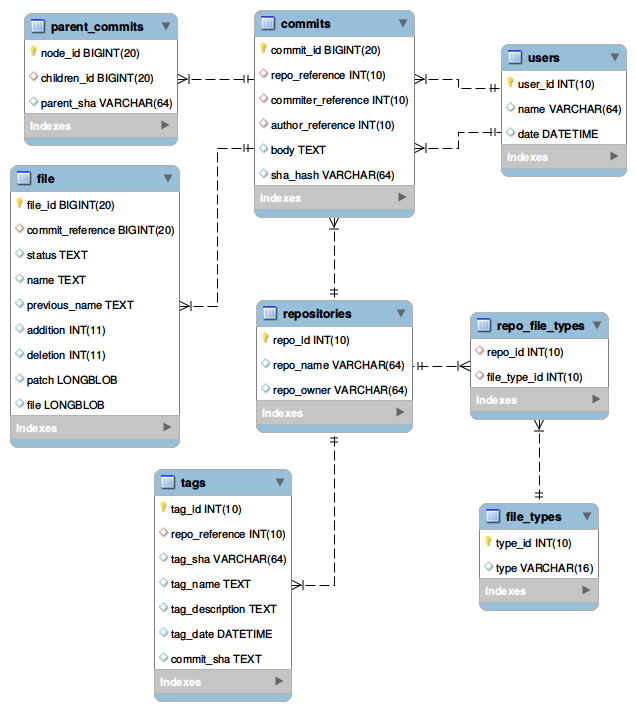
\includegraphics[width=1.0\textwidth]{images/github_data_schema}
    \caption{GitHub Data Schema}
    \label{fig:github_data_schema}
\end{figure}

%TODO re-factor this
The first database, \textit{github\_data}, stores the semi-raw data collected from GitHub's \gls{api}. This database contains 8 tables which store various aspects about the projects considered potentially important for the analysis later on. The tables of primary concern are \textit{repositories}, \textit{commits}, \textit{users}, \textit{files} and \textit{tags} tables. The complete schema is outlined in \autoref{fig:github_data_schema}. Other aspects are available from the \gls{api} and if need the database could be extended to store more elements as necessary. In some cases data from the \gls{api} is not available for one reason or another (usually inaccessible files or such) these are simply removed or a note is made of them depending on their importance. For example, files missing that already do not contain Java code are not essential and if inaccessible are ignored. If a Java file is inaccessible a note is made as this is a greater concern. These files can be retrieved if enough information is available (previous version and corresponding patch file). In the case that insufficient information is available the analysis can still be applied but will likely adversely effected the result.

After storing the data in the \textit{github\_data} database, the analysis process is done. The \textit{parsing} script is run next and discussed further in the \autoref{sec:parsing}. The results are then stored the \textit{project\_stats} database that is very similar in layout to the first database except some extra tables have been added and a few data items have been removed. Mostly the storage expansions have been to hold change information calculated from the analysis of the data. The complete schema is outlined in \autoref{fig:project_stats_schema}.

\begin{figure}[!ht]
    \centering
        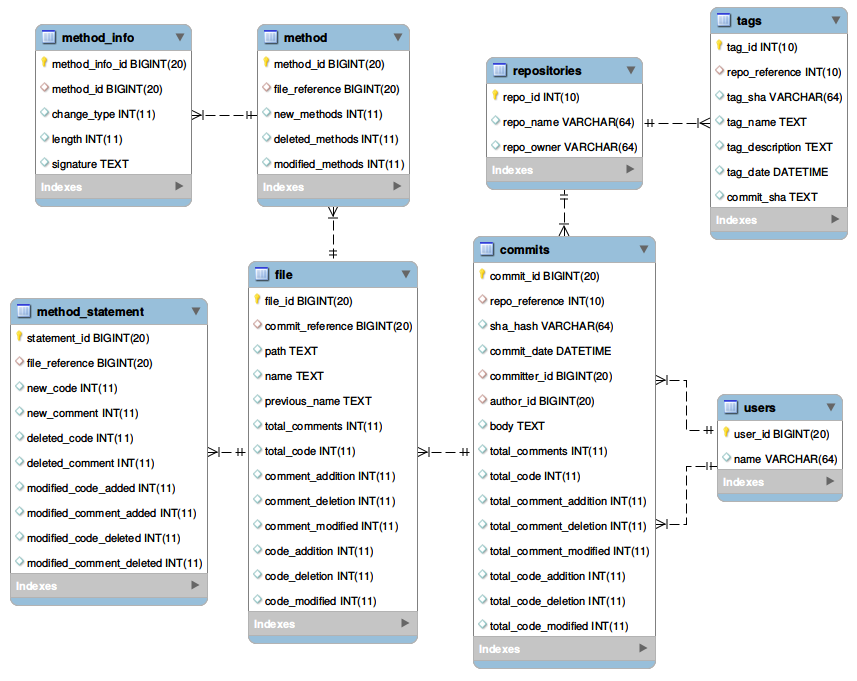
\includegraphics[width=1.0\textwidth]{images/project_stats_schema}
    \caption{Project Stats Schema}
    \label{fig:project_stats_schema}
\end{figure}

The third and final database uses PostgreSQL because of limitations within the MySQL implementation. The calculation of the candidate features, discussed in further detail in \autoref{sec:experimental_project_data}, required a more versatile partitioning function and the ability to perform multiple inner queries. The first of which is more difficult to implement and the second is not available at all MySQL. Therefore the data was transferred over to PostgreSQL, using simple program called \textit{pgloader}\footnote{\url{http://pgloader.io/}}. Only one difficulty was encountered during the transferring process. One of the tables in the MySQL database was called \textit{user}, however in PostgreSQL this is a reserved table name and therefore the table cannot be interacted with properly. The work around was to simply rename the table in MySQL prior to transferring to avoid any issues with the database. After transferring the data over to the PostgreSQL data change predictions were ready to be preformed.

\section{Parsing}
\label{sec:parsing}

The raw data collected from GitHub is stored and undergoes an analysis to extract more refined details. The process first requires the changes from a commit, the patches, to be merged into their corresponding full file. A patch is simply a stub file which summarizes the changes that occurred within a source file. Once the patch is merged with the raw source file a full file is formed that contains every change as well as the source code that did not change. Within a patch file and a full source file three different types of changes are present; additions, deletions and no change. These are represented as a plus sign, minus sign and space respective. An example of each of these changes are outlined in Figures \ref{fig:added_method}, \ref{fig:removed_method}, \ref{fig:changed_method}, \ref{fig:unchanged_method}. The coloring used within these images is purely for visual effect and not present in raw patch files.

% TODO talk about these different changes
% TODO consider getting different images (for removed, changed, and unchanged) all of them are too wide and the scaling looks terrible.
% - Fix by zooming in and then refreshing the page, make sure to get a piece of code that is not to wide.
% TODO fix these so their font is the same.
\begin{figure}[!ht]
    \centering
        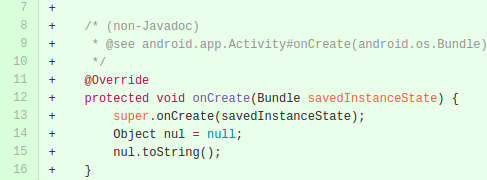
\includegraphics[width=1.0\textwidth]{images/added_example}
    \caption{Newly added method}
    \label{fig:added_method}
\end{figure}

\begin{figure}[!ht]
    \centering
        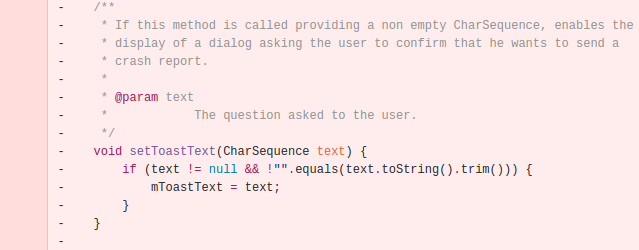
\includegraphics[width=1.0\textwidth]{images/deleted_method}
    \caption{Removed method}
    \label{fig:removed_method}
\end{figure}

\begin{figure}[!ht]
    \centering
        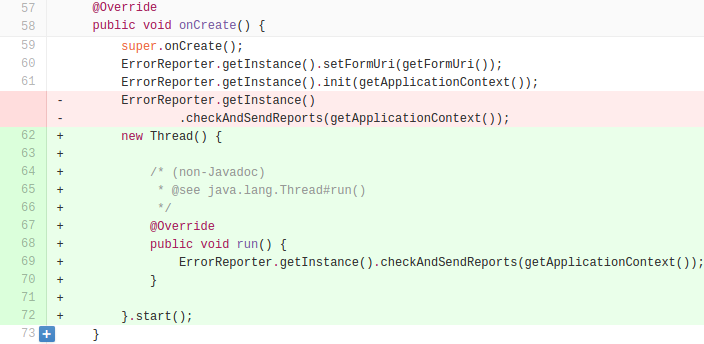
\includegraphics[width=1.0\textwidth]{images/simple_complex}
    \caption{Mixed changed method}
    \label{fig:changed_method}
\end{figure}

\begin{figure}[!ht]
    \centering
        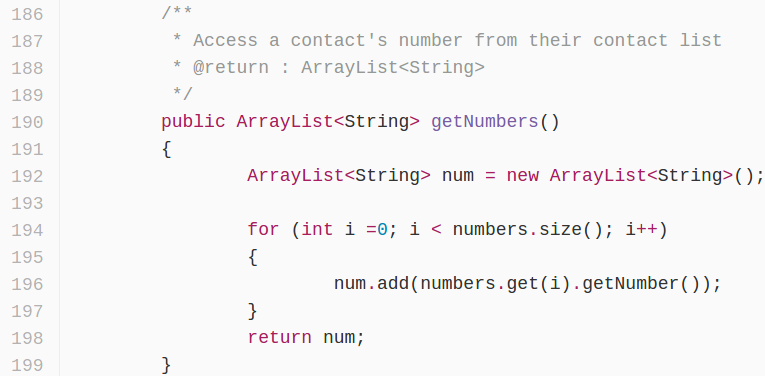
\includegraphics[width=1.0\textwidth]{images/unchanged_example}
    \caption{Unchanged method}
    \label{fig:unchanged_method}
\end{figure}

The process of reconstructing a full file using a patch file requires modifying the original source file. Since the source file used is the product of the patch file the patch must be applied in reverse. Therefore lines with a plus sign, additions, are assumed to be within the file and lines with minus signs, deletions, are assumed to not be present within the file. The lines previous removed from the source file are added back to their original location with a minus sign to preserve the original meaning of the line. The lines that were added to the source file are perpended with a plus sign identify that the line is an addition.

This full source file is then analyzed to extract each method to identify the type of change as well as other method metrics. The type of change that occurred to a method is identified as one of four possible changes. First, a method may be completely new and is thus classified as a new method shown in \autoref{fig:added_method}. The second method closely, related to the first would be an entirely removed method that is classified as a deleted method shown in \autoref{fig:removed_method}. The third classification that is more difficult method to identify is a modified method. Simply a modified method is one that contains at least two of following three change types; added, removed or unchanged lines. An example of a method that contains all three change types is shown in \autoref{fig:changed_method}. In the event that a method consists entirely of additions and deletions then the method is classified as both a new method and deleted method. A deleted and added classification is used over a modified classification because if all lines are deleted and re-added then the method is change far more drastic than a simple modification. The final change type is that of no change, where the method does not contain any changes and is shown in \autoref{fig:unchanged_method}.

For each commit this information is stored to allow for easier access and save time since the analysis of larger datasets can be time intensive. In order to maintain the integrity of the initial dataset this information is stored in a new database. There are several other features available in the data set from the extraction process beyond the ones outlined here in detail. A few of those features include the commit author, the commit message and the method length per commit. This data is stored in the database to help create the prediction model later on.

\section{Visualization}

\subsection{Line Change}
\label{subsec:line_change}

After collecting and analyzing the data the key features are extracted from the collected data. In order to to better understand resulting data it was visualized. The first visualization simply showed the changes recorded on a per line basis. These changes were divided into several closely related subcategories of additions, deletions and modifications. Additions identify changes that are new and do not have a corresponding set of deleted code. Similarly deletions refers to changes that remove code without a corresponding set of additions. Finally modifications are a set of changes which contain a set of additions and deletions that are related.

In a modification the changes are related through the \gls{ld} calculation. This distance calculation will determine the edit distance between two strings. Where edit distance is defined as the number of characters difference between two different strings. For example, \gls{ld} between \textit{happy} and \textit{mapper} would be 3, since h would be changed to m, y to e and r would be added at the end. While this provides a good initial method for comparison between two string values the value must be normalized to allow for more general use. To calculate \gls{nld} the \gls{ld} would be divided by the larger of the two strings sizes shown in \autoref{eq:normalized_ld}.

% TODO note that a_i is an addition line and that d_j is a deletion line
% TODO clarify change block with picture

\begin{equation}
\label{eq:normalized_ld}
NLD(a_i, d_j) = \frac{LD(a_i, d_j)}{\max(|a_i|,|d_j|)}
\end{equation}

% TODO show distance calculation and paper cite this.
Modifications were assumed to only take place in a series of changes that involved both additions and deletions shown in \autoref{fig:changed_method} and with an \gls{nld} below a defined threshold $\Delta_m$.

\begin{equation}
\label{eq:similarity_threshold}
m(a_i, d_j) = NLD(a_i, d_j) < \Delta_m
\end{equation}

In order to account for larger method signatures a threshold $\alpha$ was created to separate small and large method signatures. Therefore the \autoref{eq:similarity_threshold} was updated accordingly shown in \autoref{eq:complete_similarity_threshold}.

\begin{equation}
\label{eq:complete_similarity_threshold}
m(a_i, d_j) = \left\{\begin{matrix}
NLD(a_i, d_j) < \Delta_s & \text{if } \max(|a_i|, |d_j|) < \alpha \\ 
NLD(a_i, d_j) < \Delta_l & \text{otherwise}
\end{matrix}\right.
\end{equation}

Lines that are part of the same block of additions and deletions are selected for the similarity check to determine whether they can be classified as a modification. Modifications will consist of one to many addition lines mapped to one to many lines of deletion. Therefore a modification is more easily referred to as a modification set.

For addition lines that do not meet the threshold of similarity with any deletion line in the change block are classified as additions. Similarly, deletion lines who fail to meet the similarity threshold for any addition lines will be classified as deletions. Therefore a block of changes will contain a set of additions, deletions and modifications any of which may be empty.

% TODO talk about comments.

% TODO talk about the summary stats

% Discuss the slight controls that each one allows and the special one just for this view. TODO place this better.
The project's tags are shown at the bottom of each graph optionally to potentially provide some context. Since these tags often mark points of significant within the project they can be thought as road signs. The site also provides some options to refine or generalize the graphs. For all of the graphs you are allowed to select the project, package path, and the committers you wish to view. Specifically for the line level graph a further option is provided to condense the data based on a monthly, weekly summary.

% TODO fit in the commit information shown
As a further guide marker the commit information is provided (when viewing either line at the commit view, method level or statement level). This information allows for a direct link to the project and can be a handy tool for referring back to the software repository.

% \begin{figure}[!ht]
%     \centering
%         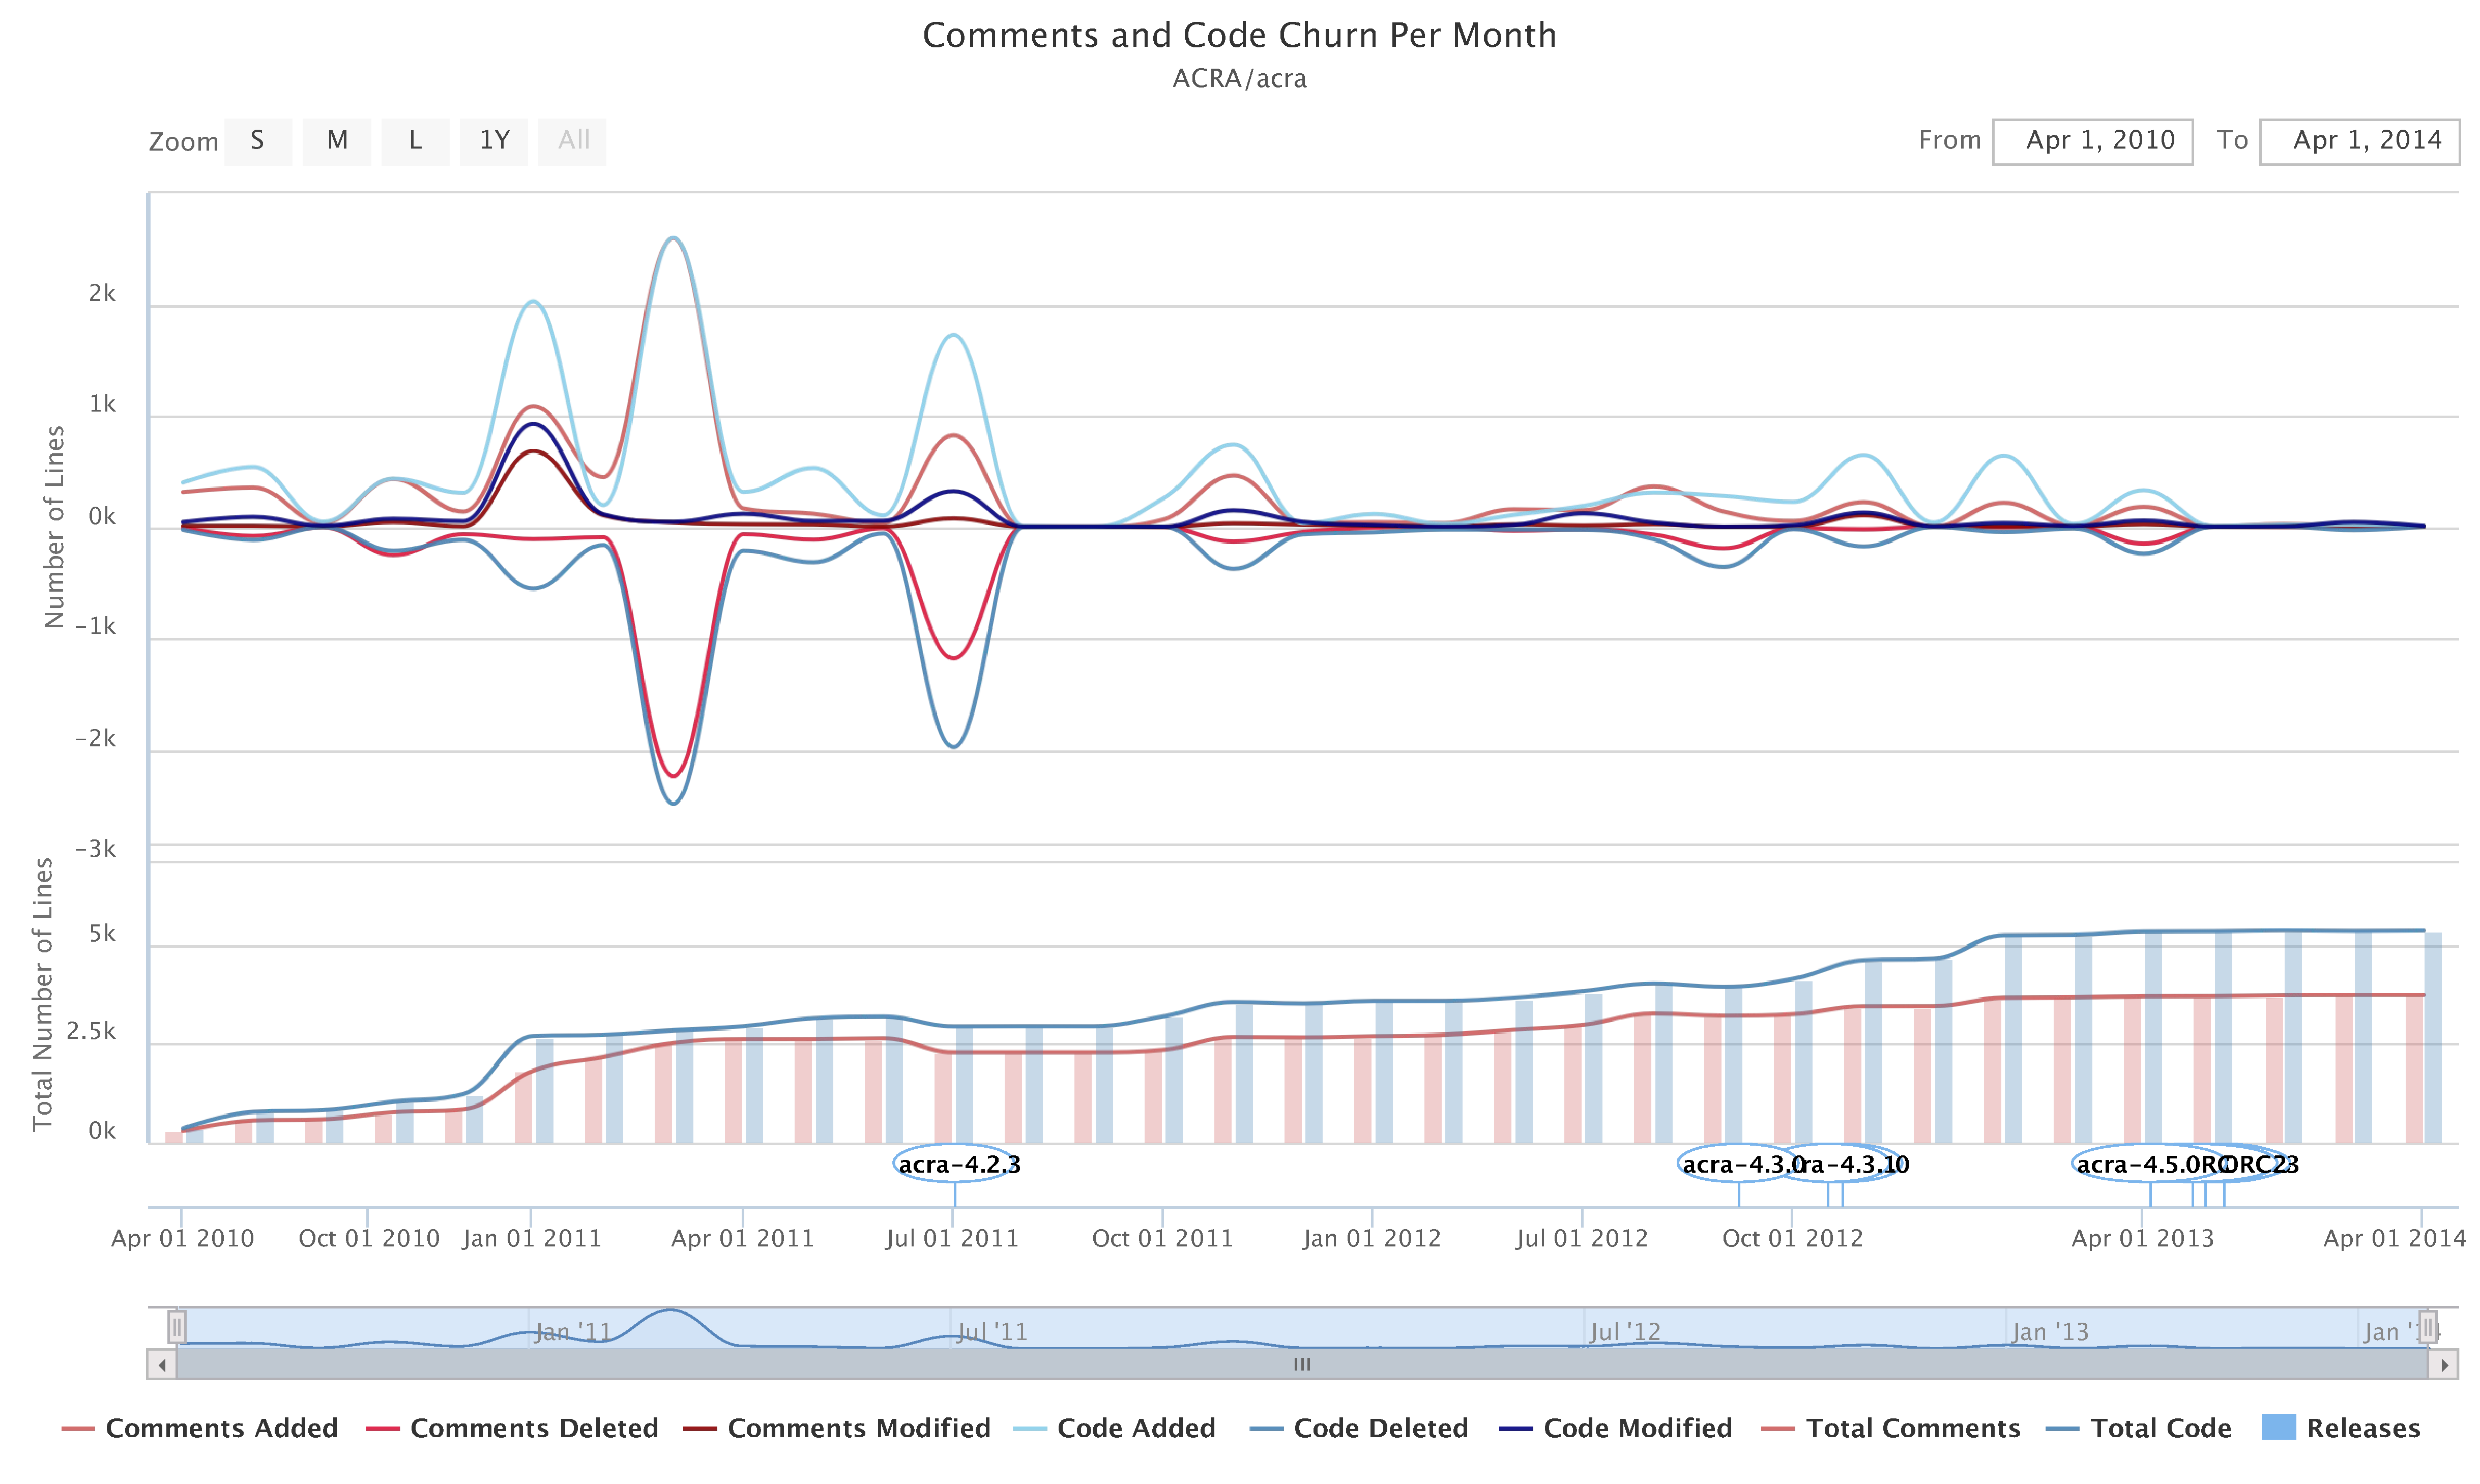
\includegraphics[width=1.0\textwidth]{images/lines_visual_acra}
%     \caption{Line Change Visualization for acra}
%     \label{fig:line_visual_acra}
% \end{figure}


\begin{landscape}
 \thispagestyle{empty}
 \begin{figure}
  \centering
        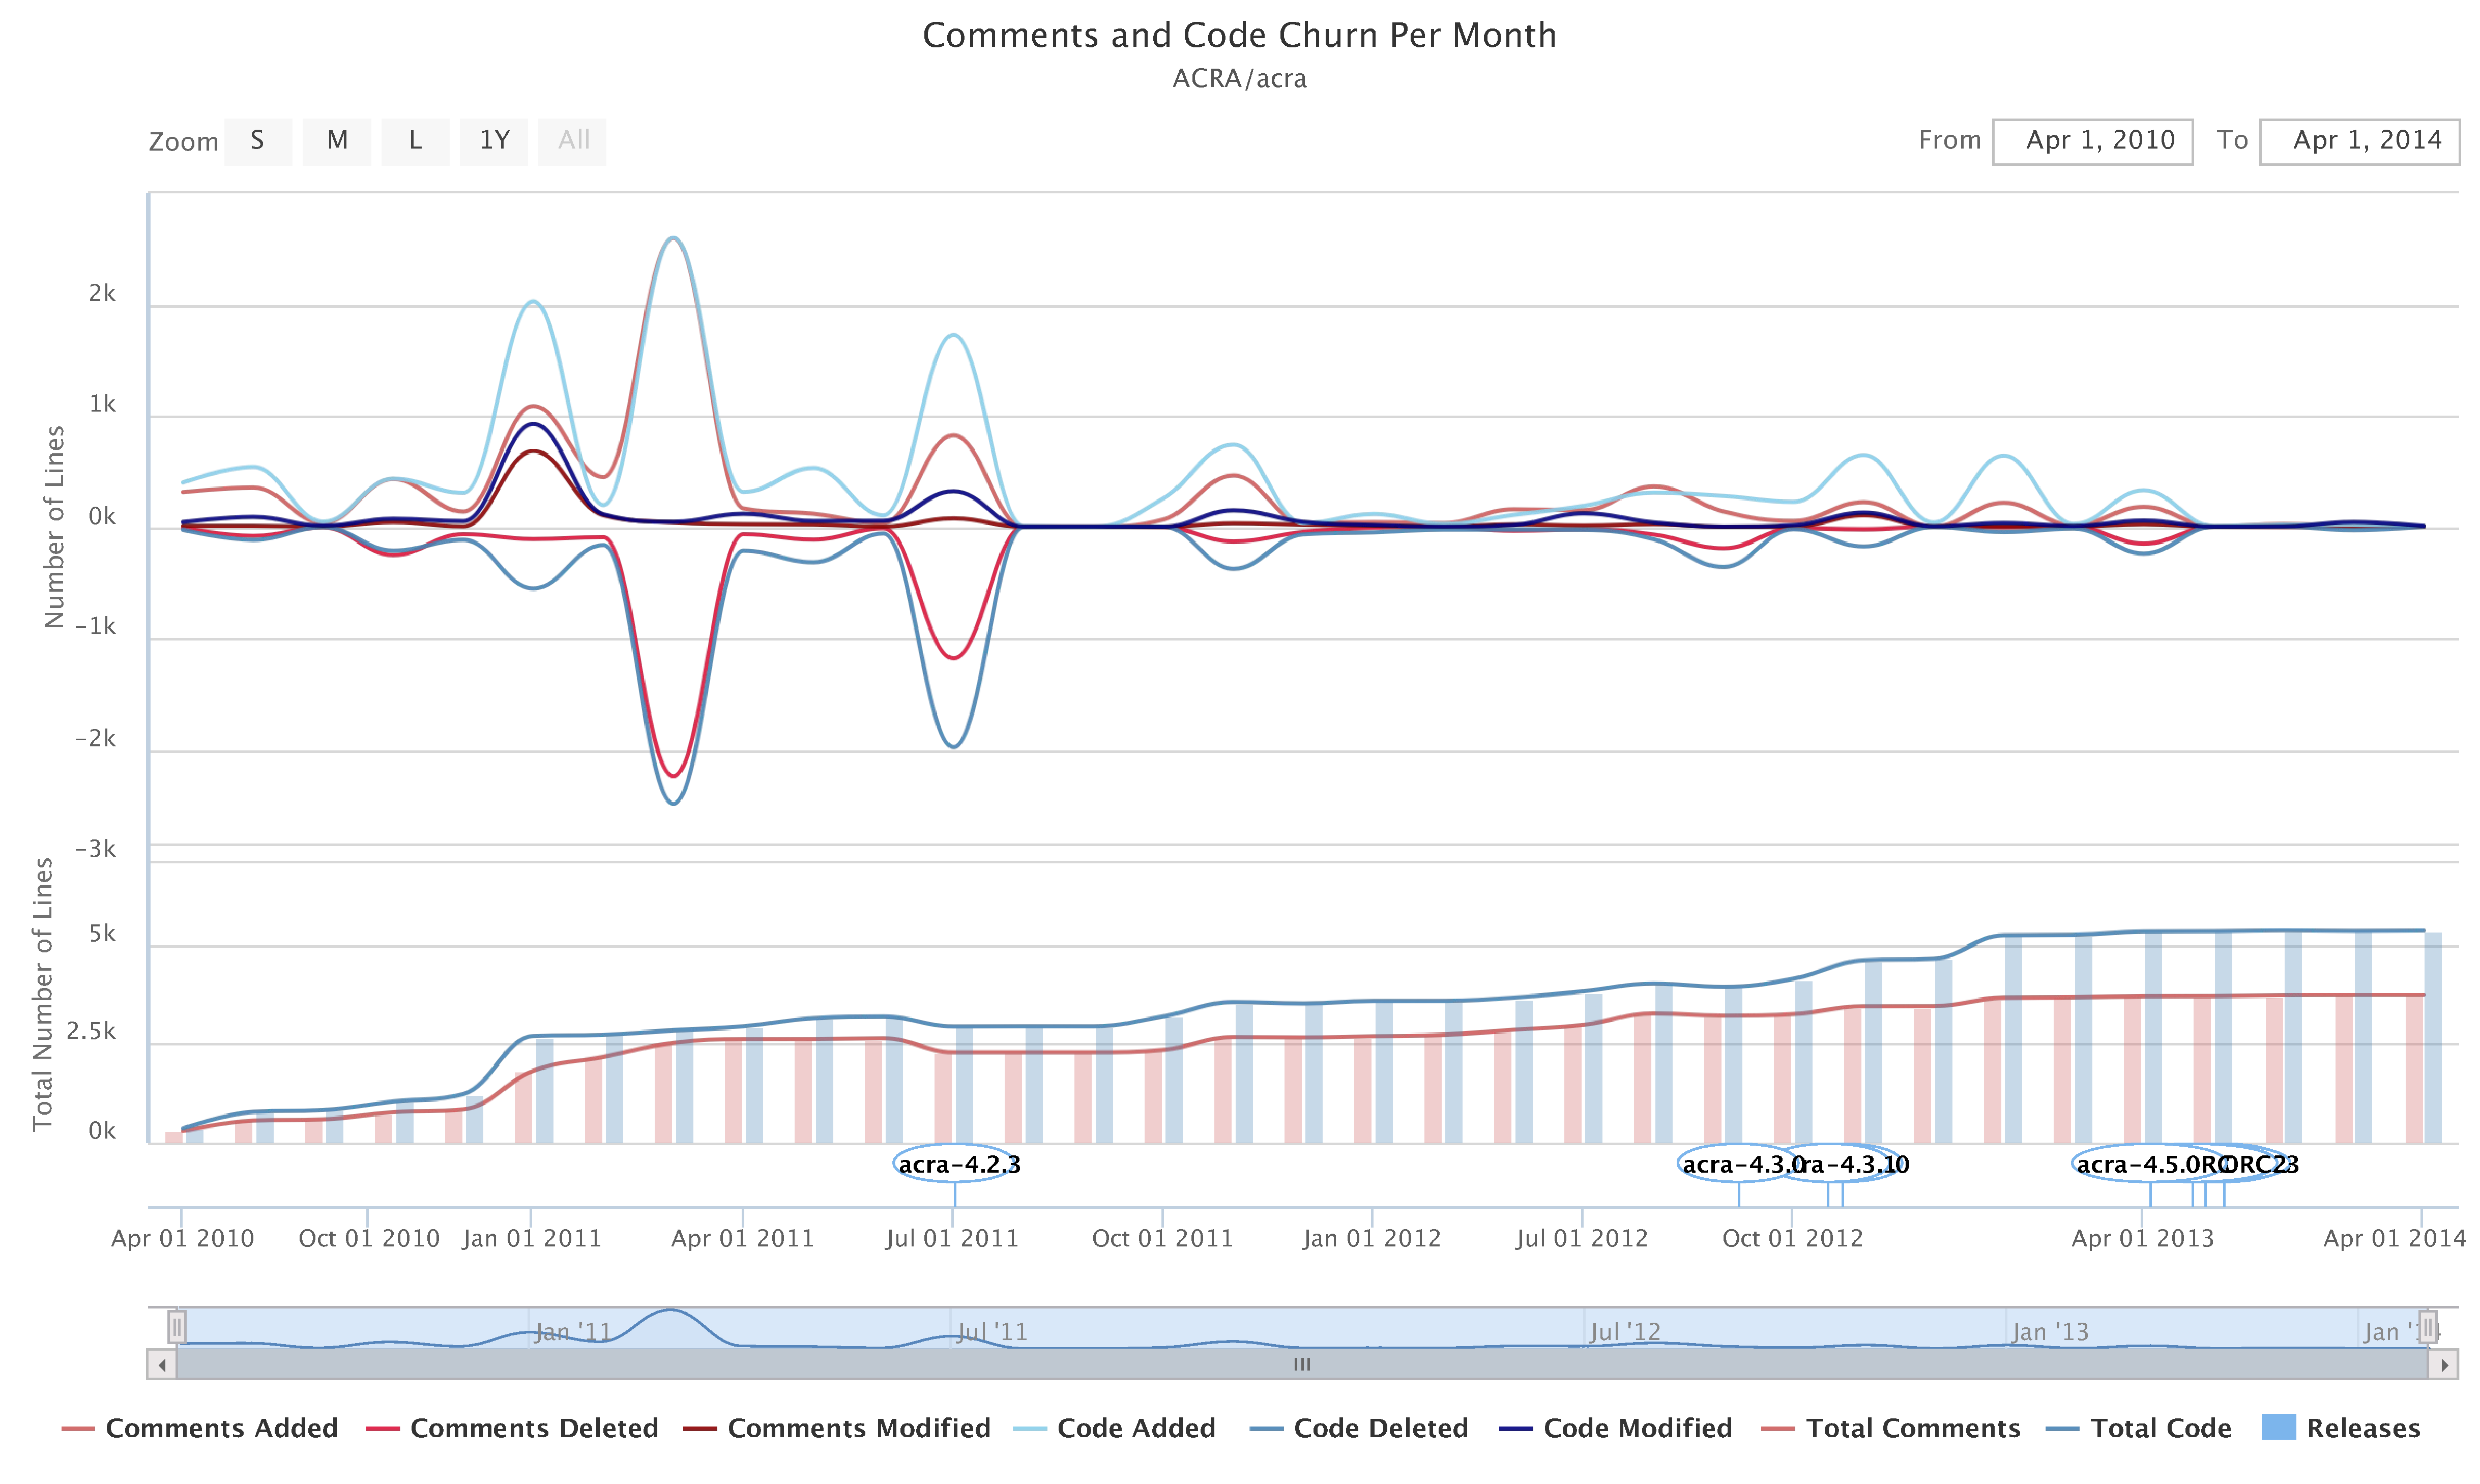
\includegraphics[width=1.5\textwidth]{images/lines_visual_acra}
    \caption{Line Change Visualization for acra}
    \label{fig:line_visual_acra}
 \end{figure}
\end{landscape}
\pagestyle{plain}

% TODO put this in the right location
% TODO talk about this.
\begin{landscape}
\thispagestyle{empty}
 \begin{figure}
  \centering
        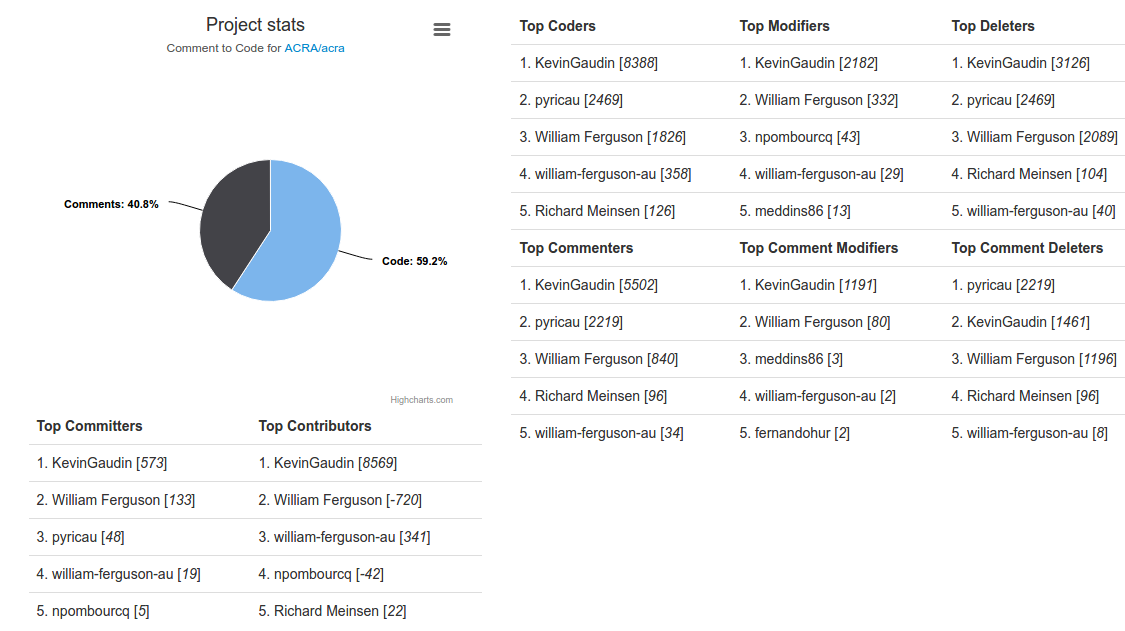
\includegraphics[width=1.5\textwidth]{images/table_visual}
    \caption{Project Summary Statistics for acra}
    \label{fig:project_summary_stats}
 \end{figure}
\end{landscape}
\pagestyle{plain}

\subsection{Method Change}

The visualization of line changes was very noisy and proved difficult to use. Instead of viewing every line of change separately they were grouped together based on the method from which they originate from. Similar classifications are used for method changes however their definitions vary slightly. There are three types of method level changes that can occur. Firstly, a method can be newly added implying that the method had not existed in the previous version. Secondly, a deleted method implying that the method is completely removed from the current version. Thirdly, a method can be modified by containing a set of changes that are not constituting the entire method changing. 
% TODO show example of each.

It should be noted that at the method level comment changes are ignored. Instead the focus is placed on that of the three types of changes. The visualization for the method level uses a bar graph since it provided a more clear picture of the relationship between commits. Rather than as the first visualization did imply that a relationship was to be drawn between different commits of the same type only changes of the same time are grouped together. The contrast in magnitude between each type of change and each commit is also more clear and defines the visualization.

% \begin{sidewaysfigure}[ht]
%     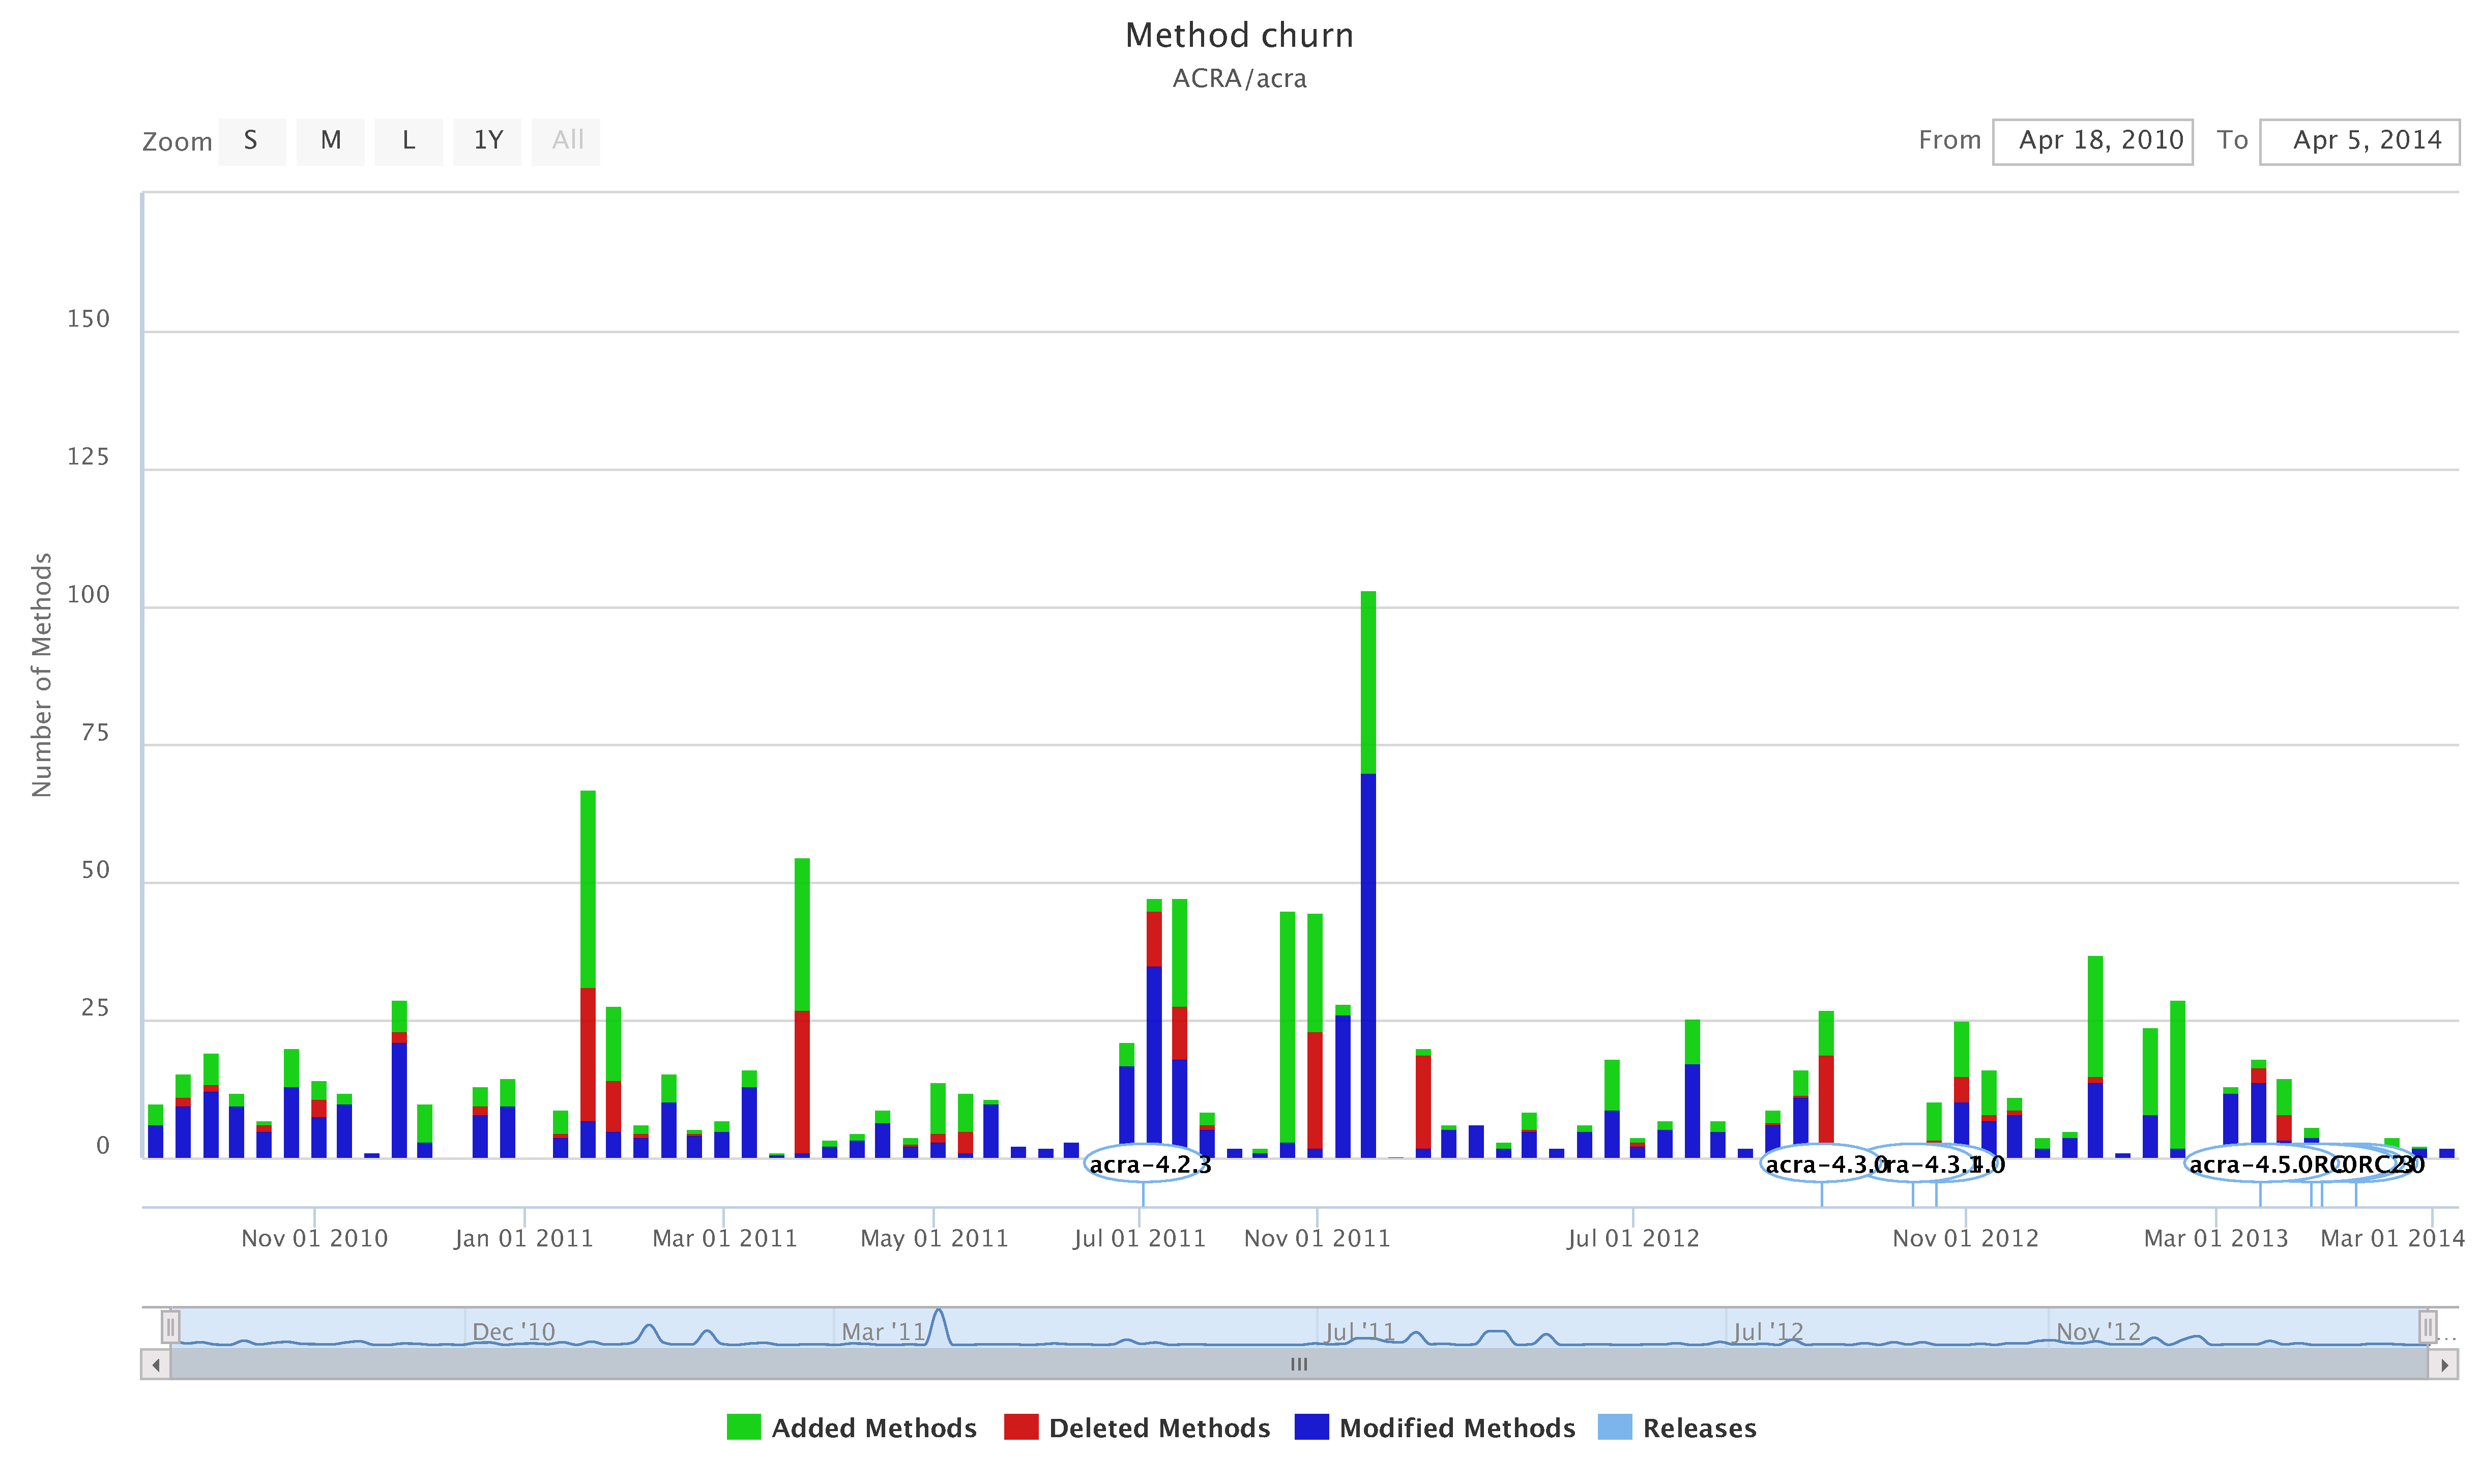
\includegraphics[width=1.0\textwidth]{images/method_visual_acra}
%     \caption{Method Change Visualization for acra}
%     \label{fig:method_visual_acra}
% \end{sidewaysfigure}

\begin{landscape}
\thispagestyle{empty}
 \begin{figure}
  \centering
    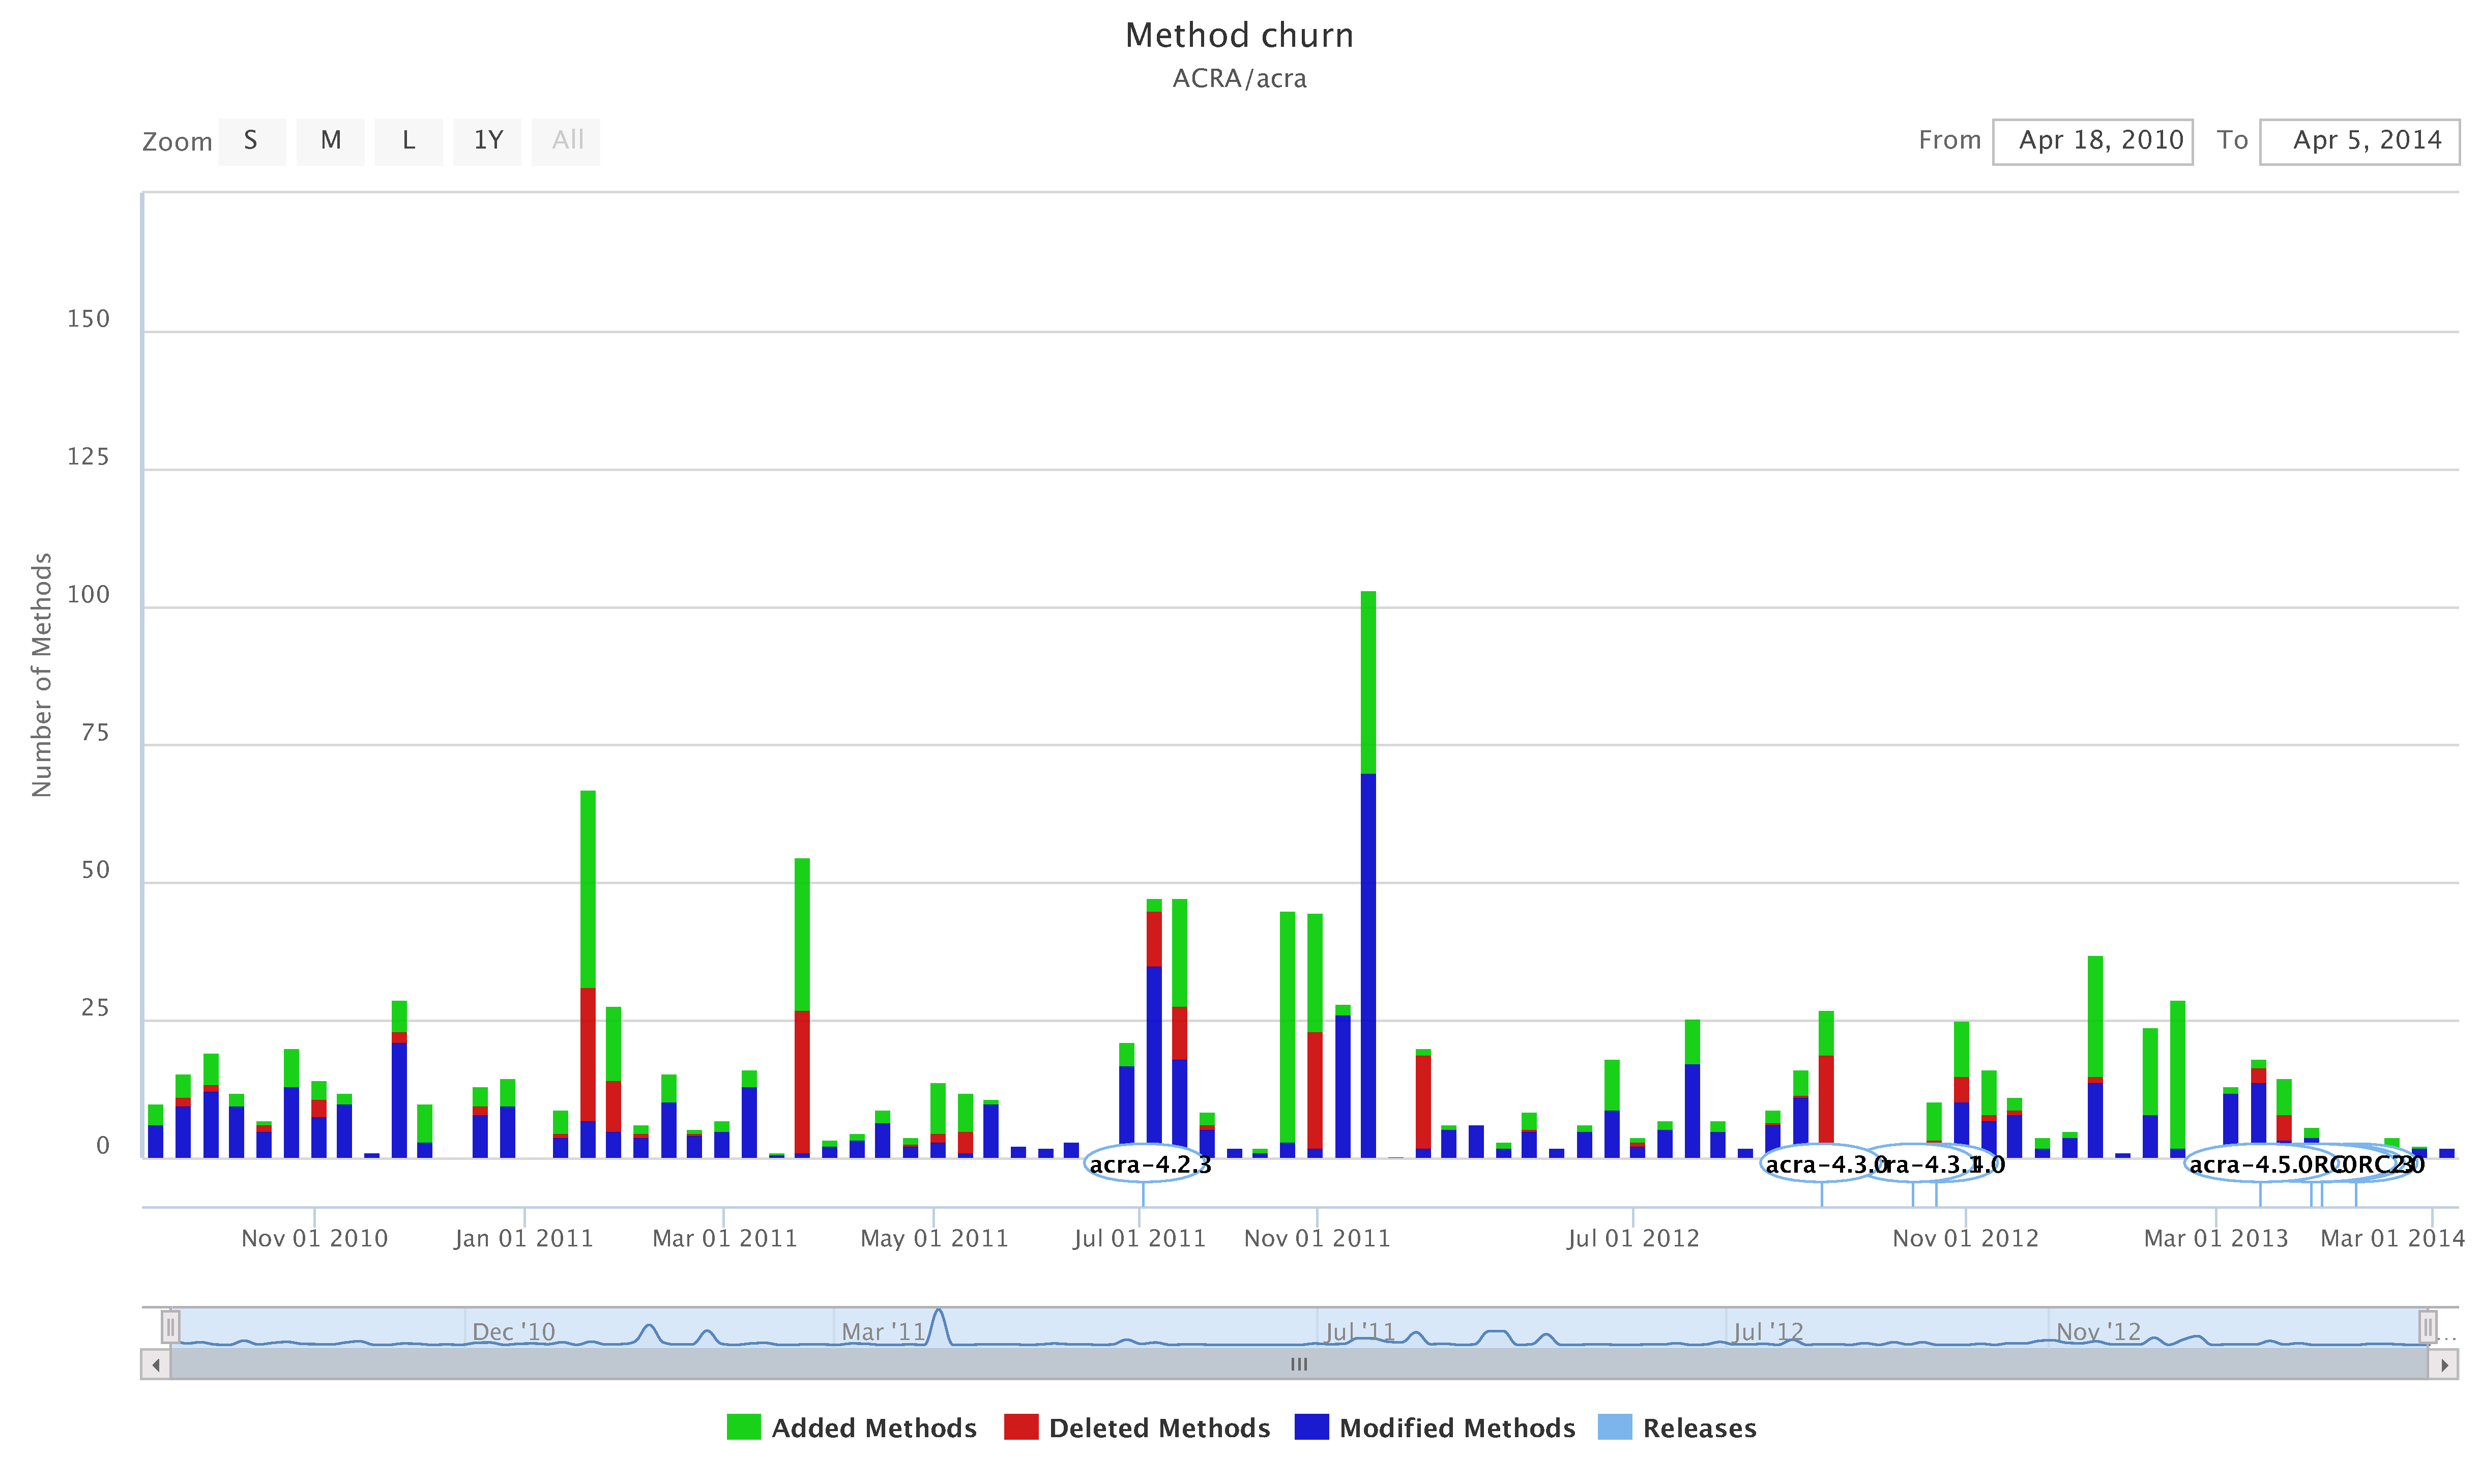
\includegraphics[width=1.5\textwidth]{images/method_visual_acra}
    \caption{Method Change Visualization for acra}
    \label{fig:method_visual_acra}
 \end{figure}
\end{landscape}
\thispagestyle{plain}

% \begin{figure}[!ht]
%     \centering
%     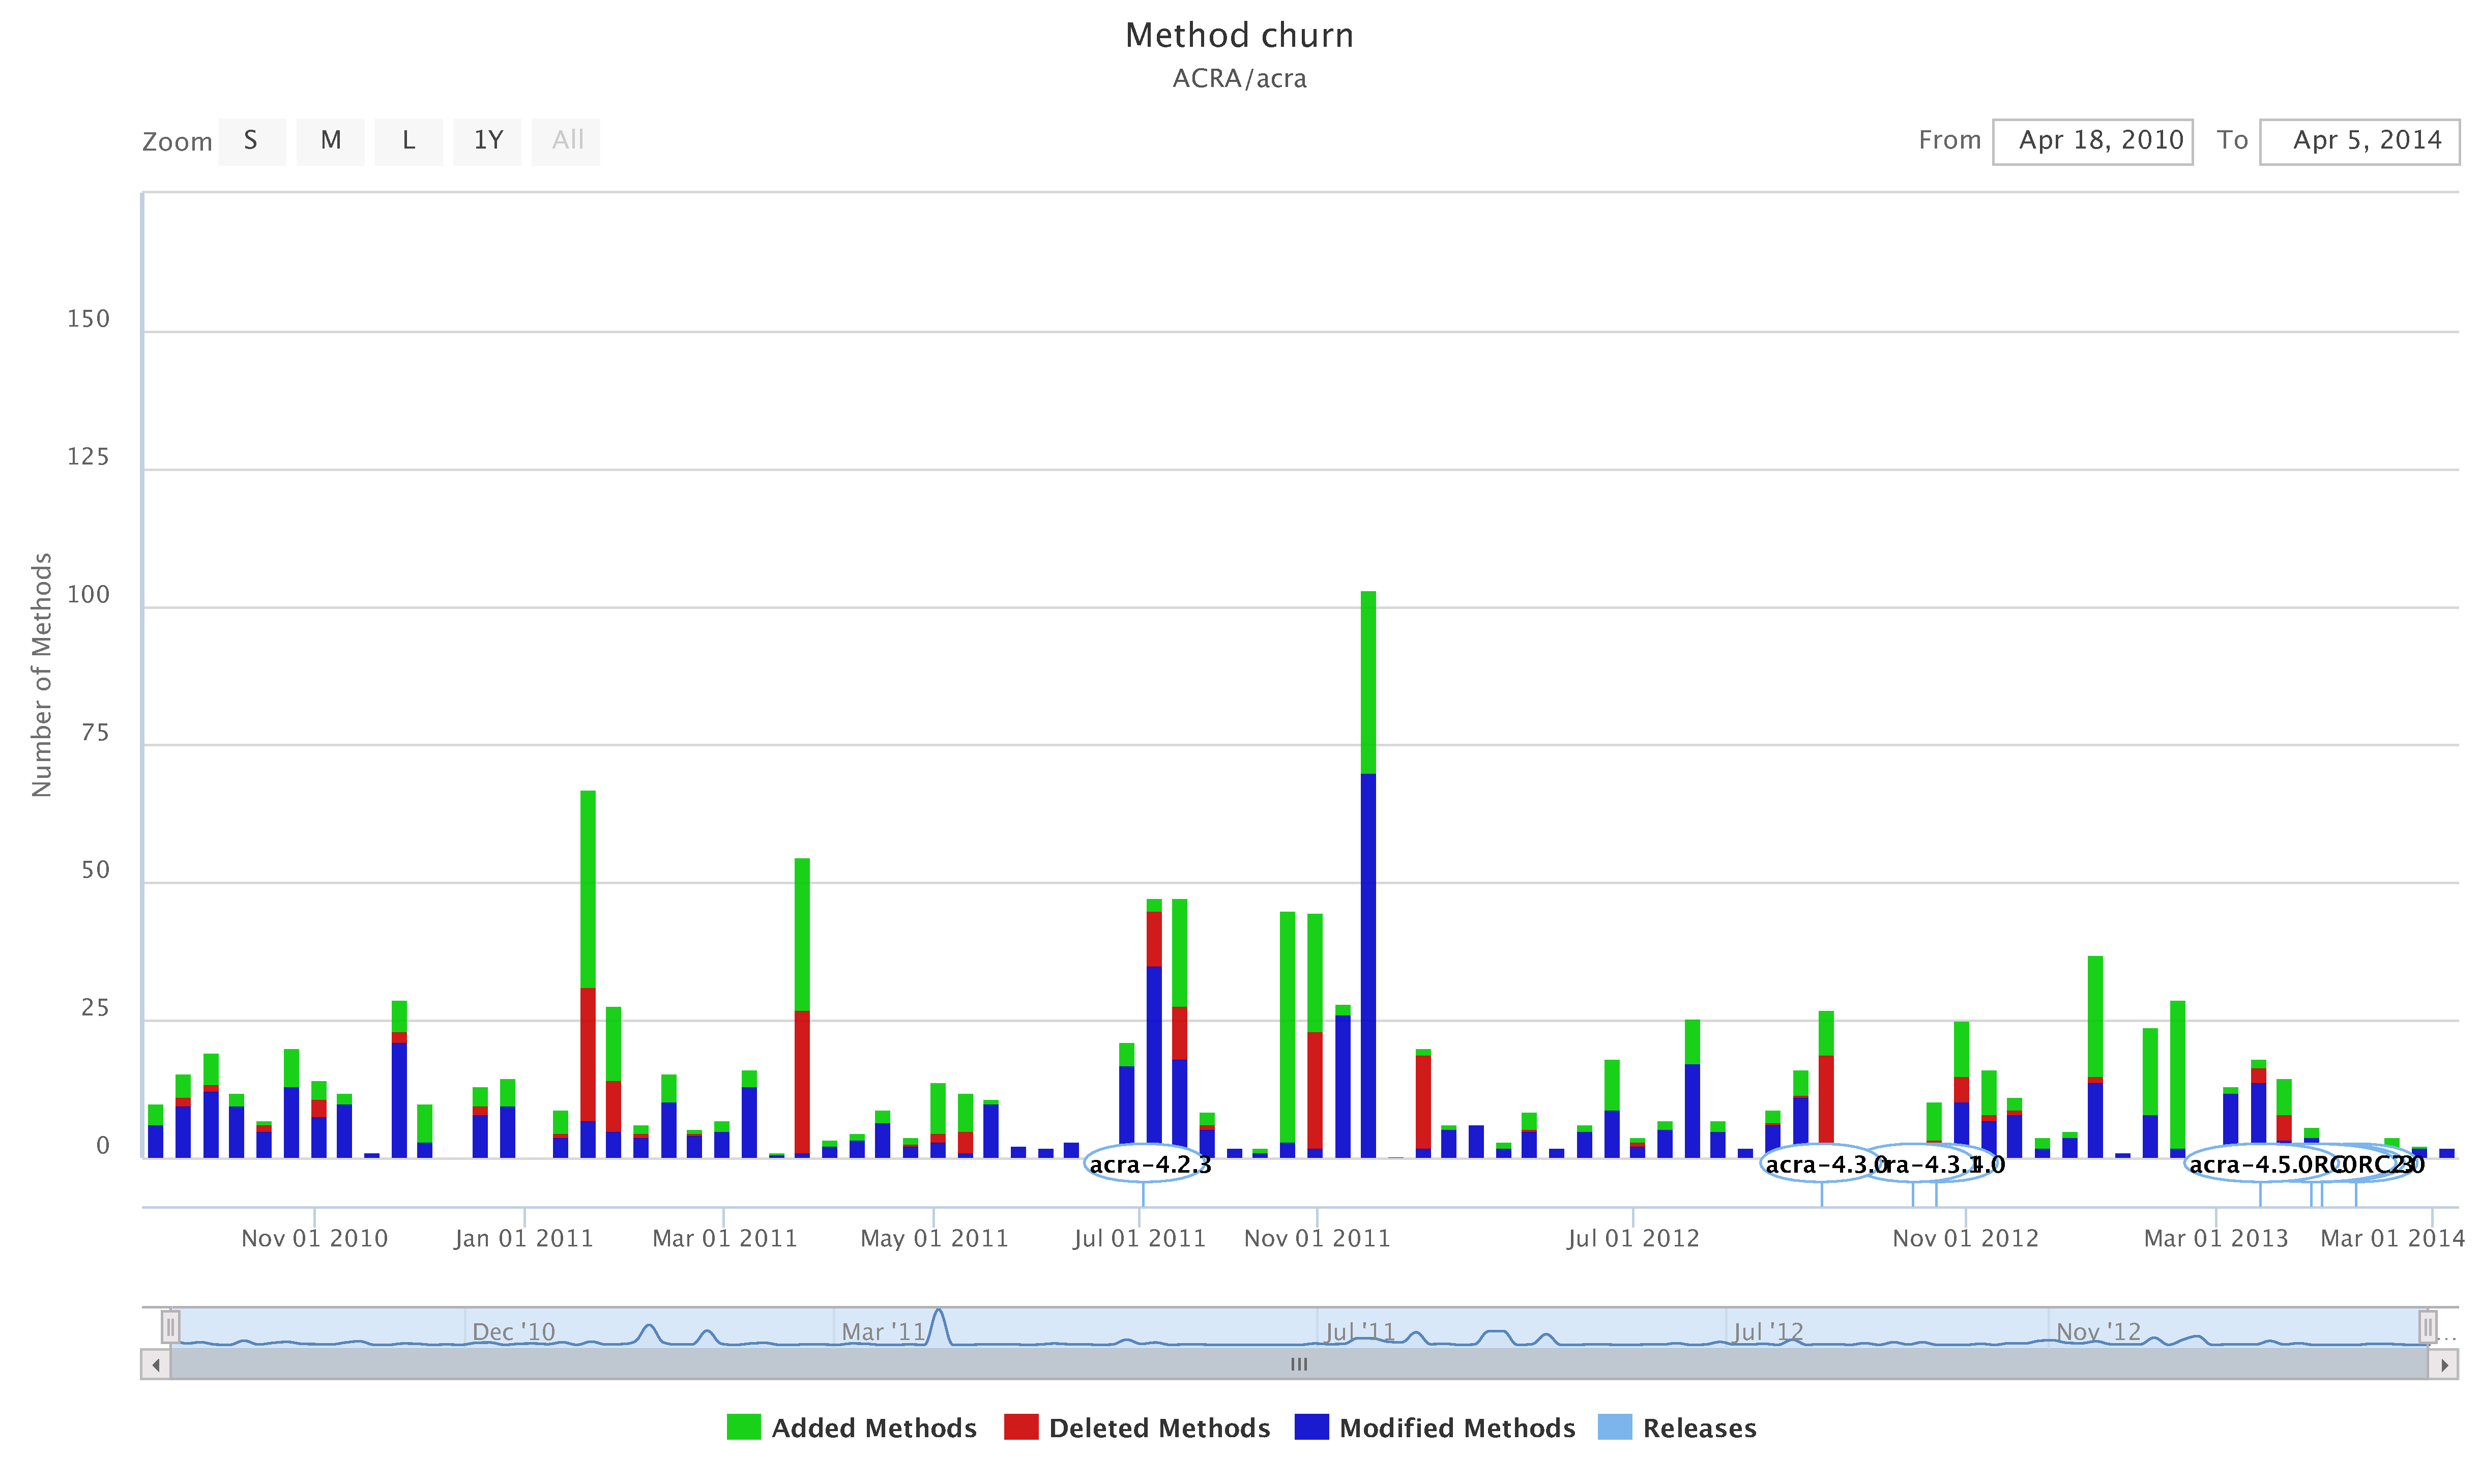
\includegraphics[width=1.0\textwidth]{images/method_visual_acra}
%     \caption{Method Change Visualization for acra}
%     \label{fig:method_visual_acra}
% \end{figure}

\subsection{Method Statement Change}

The method level visualization provided a fairly clear higher level view of the data. However, while collecting that data lower level data was collected as part of the previous analysis. This afforded a combination of the previous two methods. While more data is available and is quite overwhelming the final graph could provide some use when used in conjunction with the previous graph.

The view itself classifies changes into several categories, first their is \textit{Added} changes which comes in the form of both code and comments. Secondly, \textit{Deleted} changes which again is for both code and comments. Similar to that of the method level added or deleted method these statements belong to methods that are either entirely added or deleted from the project. However for this level each statement is counted versus just the method on whole.

The more complicated categories are introduced as part of the modification classifications. These all stem from the method level modifications. A modified method will contain some changes which can be statement additions or deletions. Therefore modifications are divided into modifications that are additions and ones that are deletions. The final filter is again based on statements being either comments are code. So finally we have the categories: \textit{Modified Code Added}, \textit{Modified Comment Added}, \textit{Modified Code Deleted} and \textit{Modified Comment Deleted}.

% \begin{figure}[!ht]
%     \centering
%         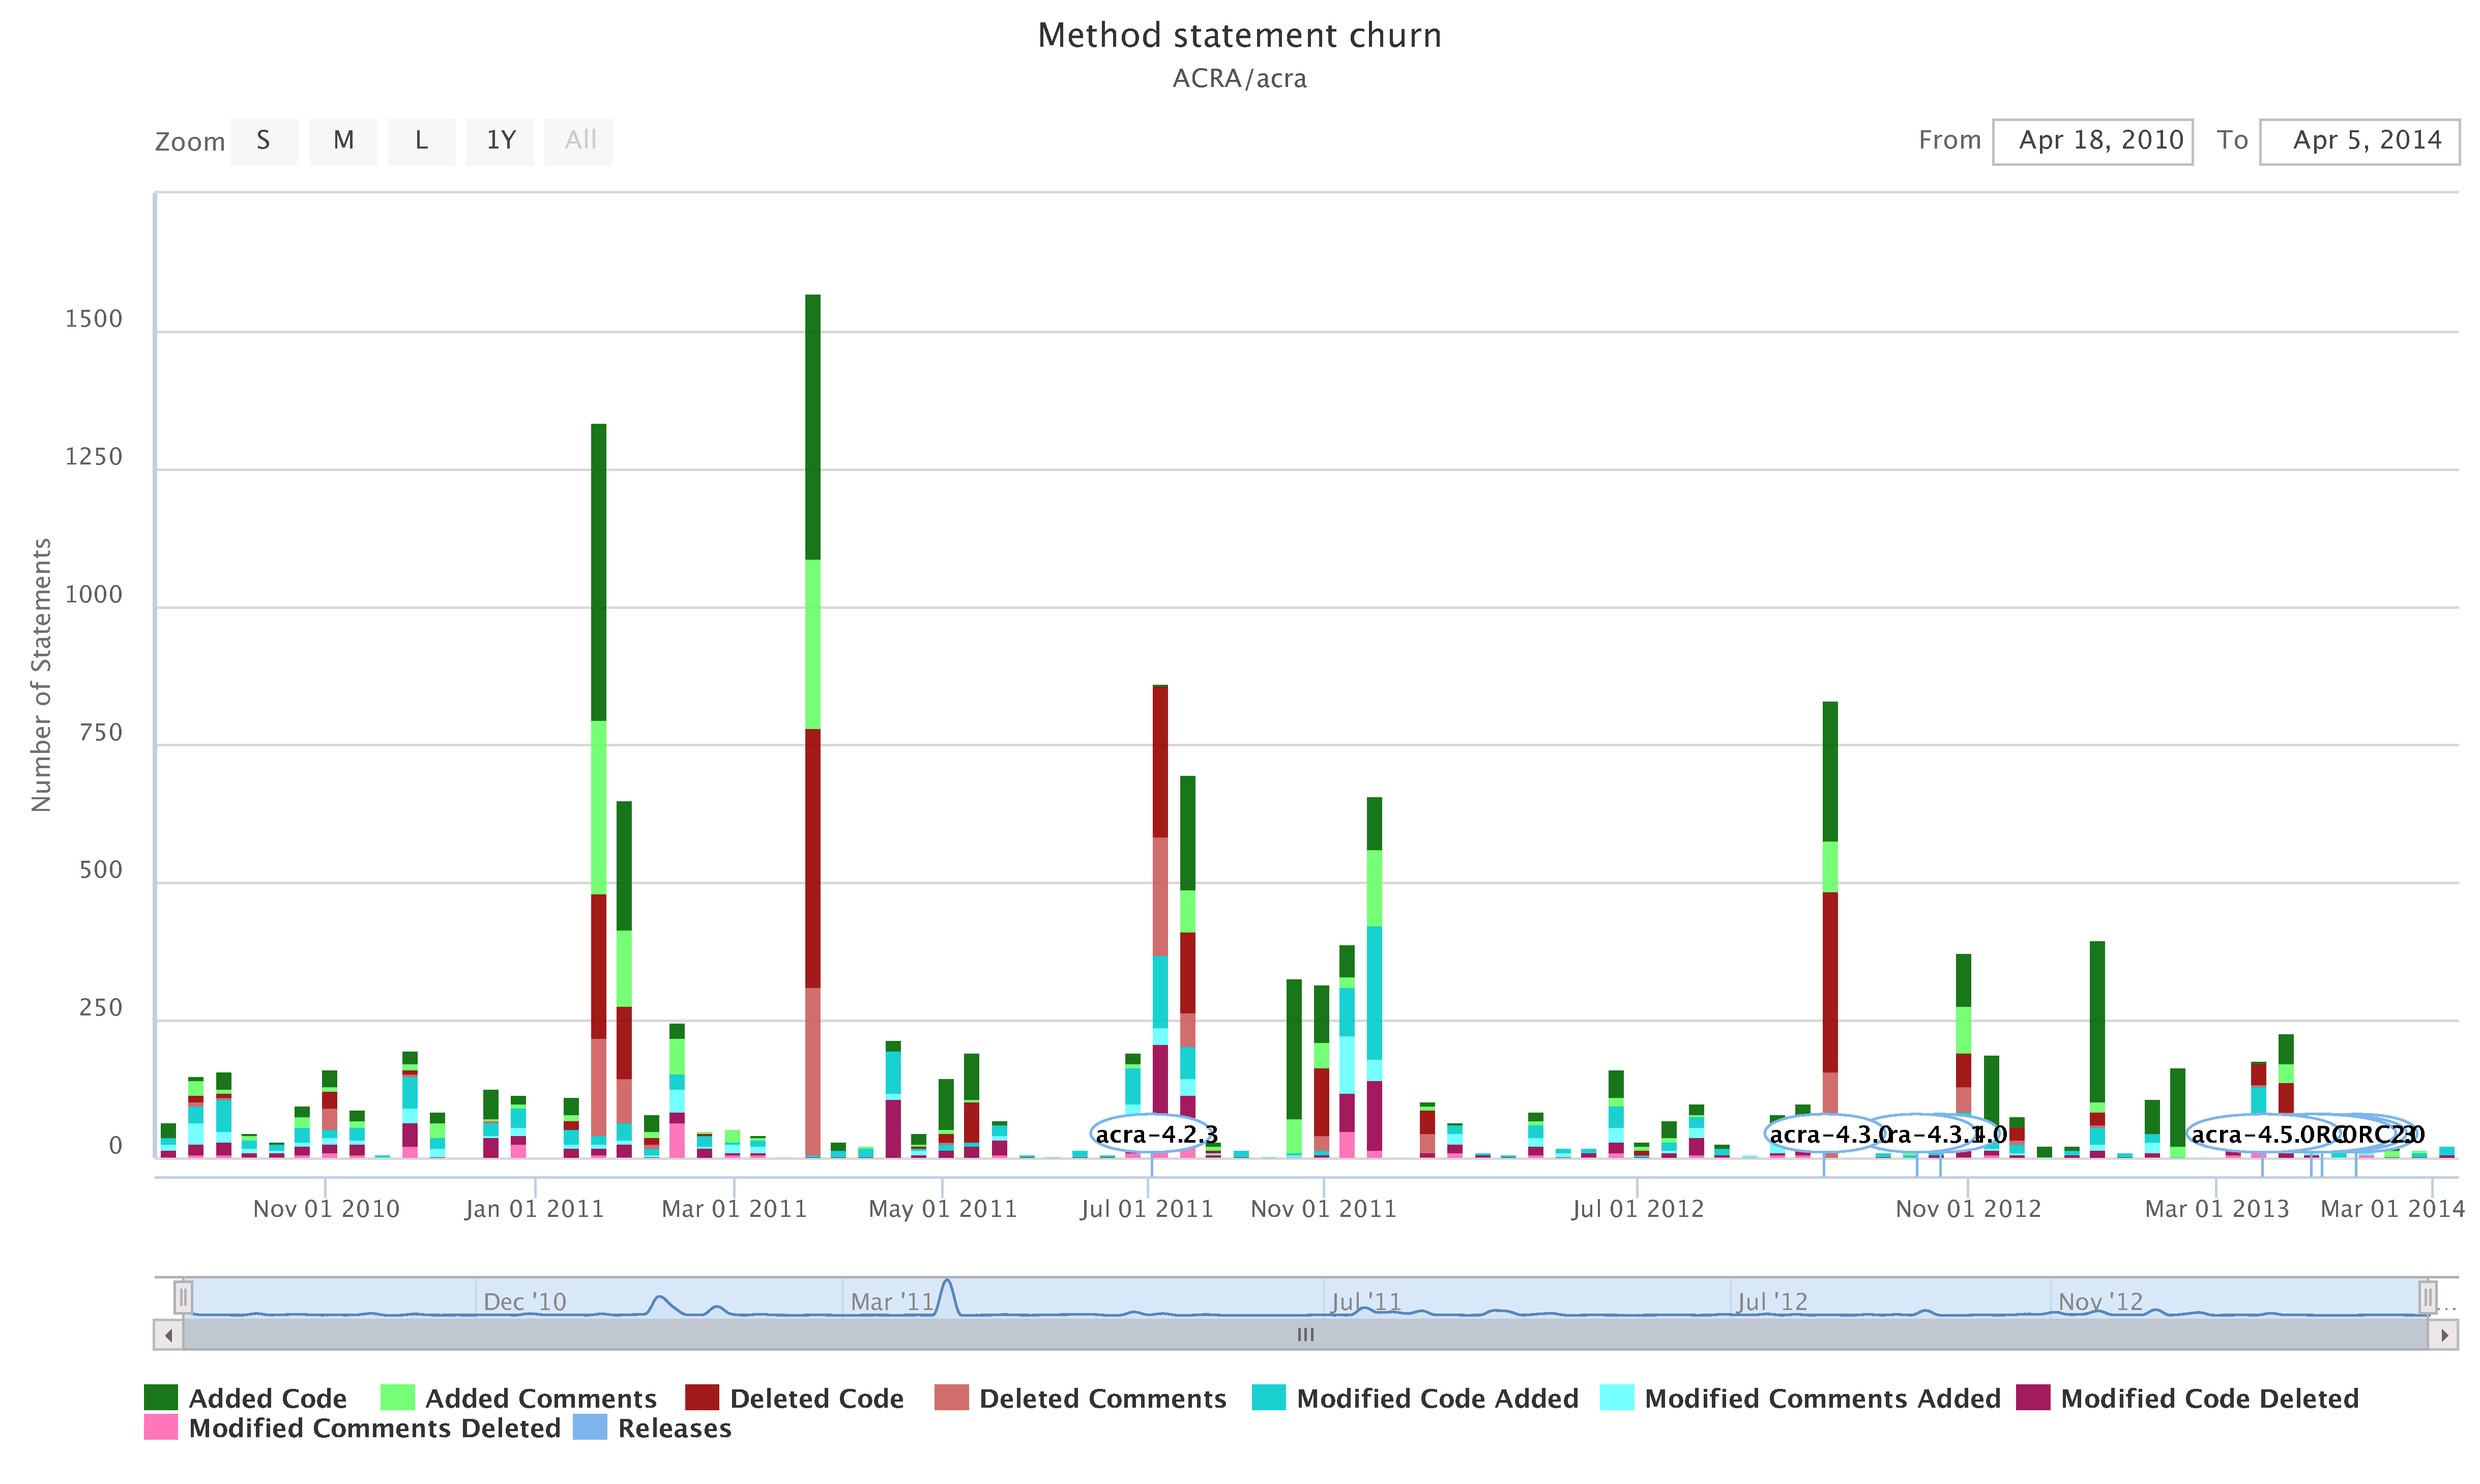
\includegraphics[width=1.0\textwidth]{images/statement_visual_acra}
%     \caption{Method Statement Change Visualization for acra}
%     \label{fig:statement_visual_acra}
% \end{figure}

% \begin{landscape}
%  \begin{figure}
%   \centering
%     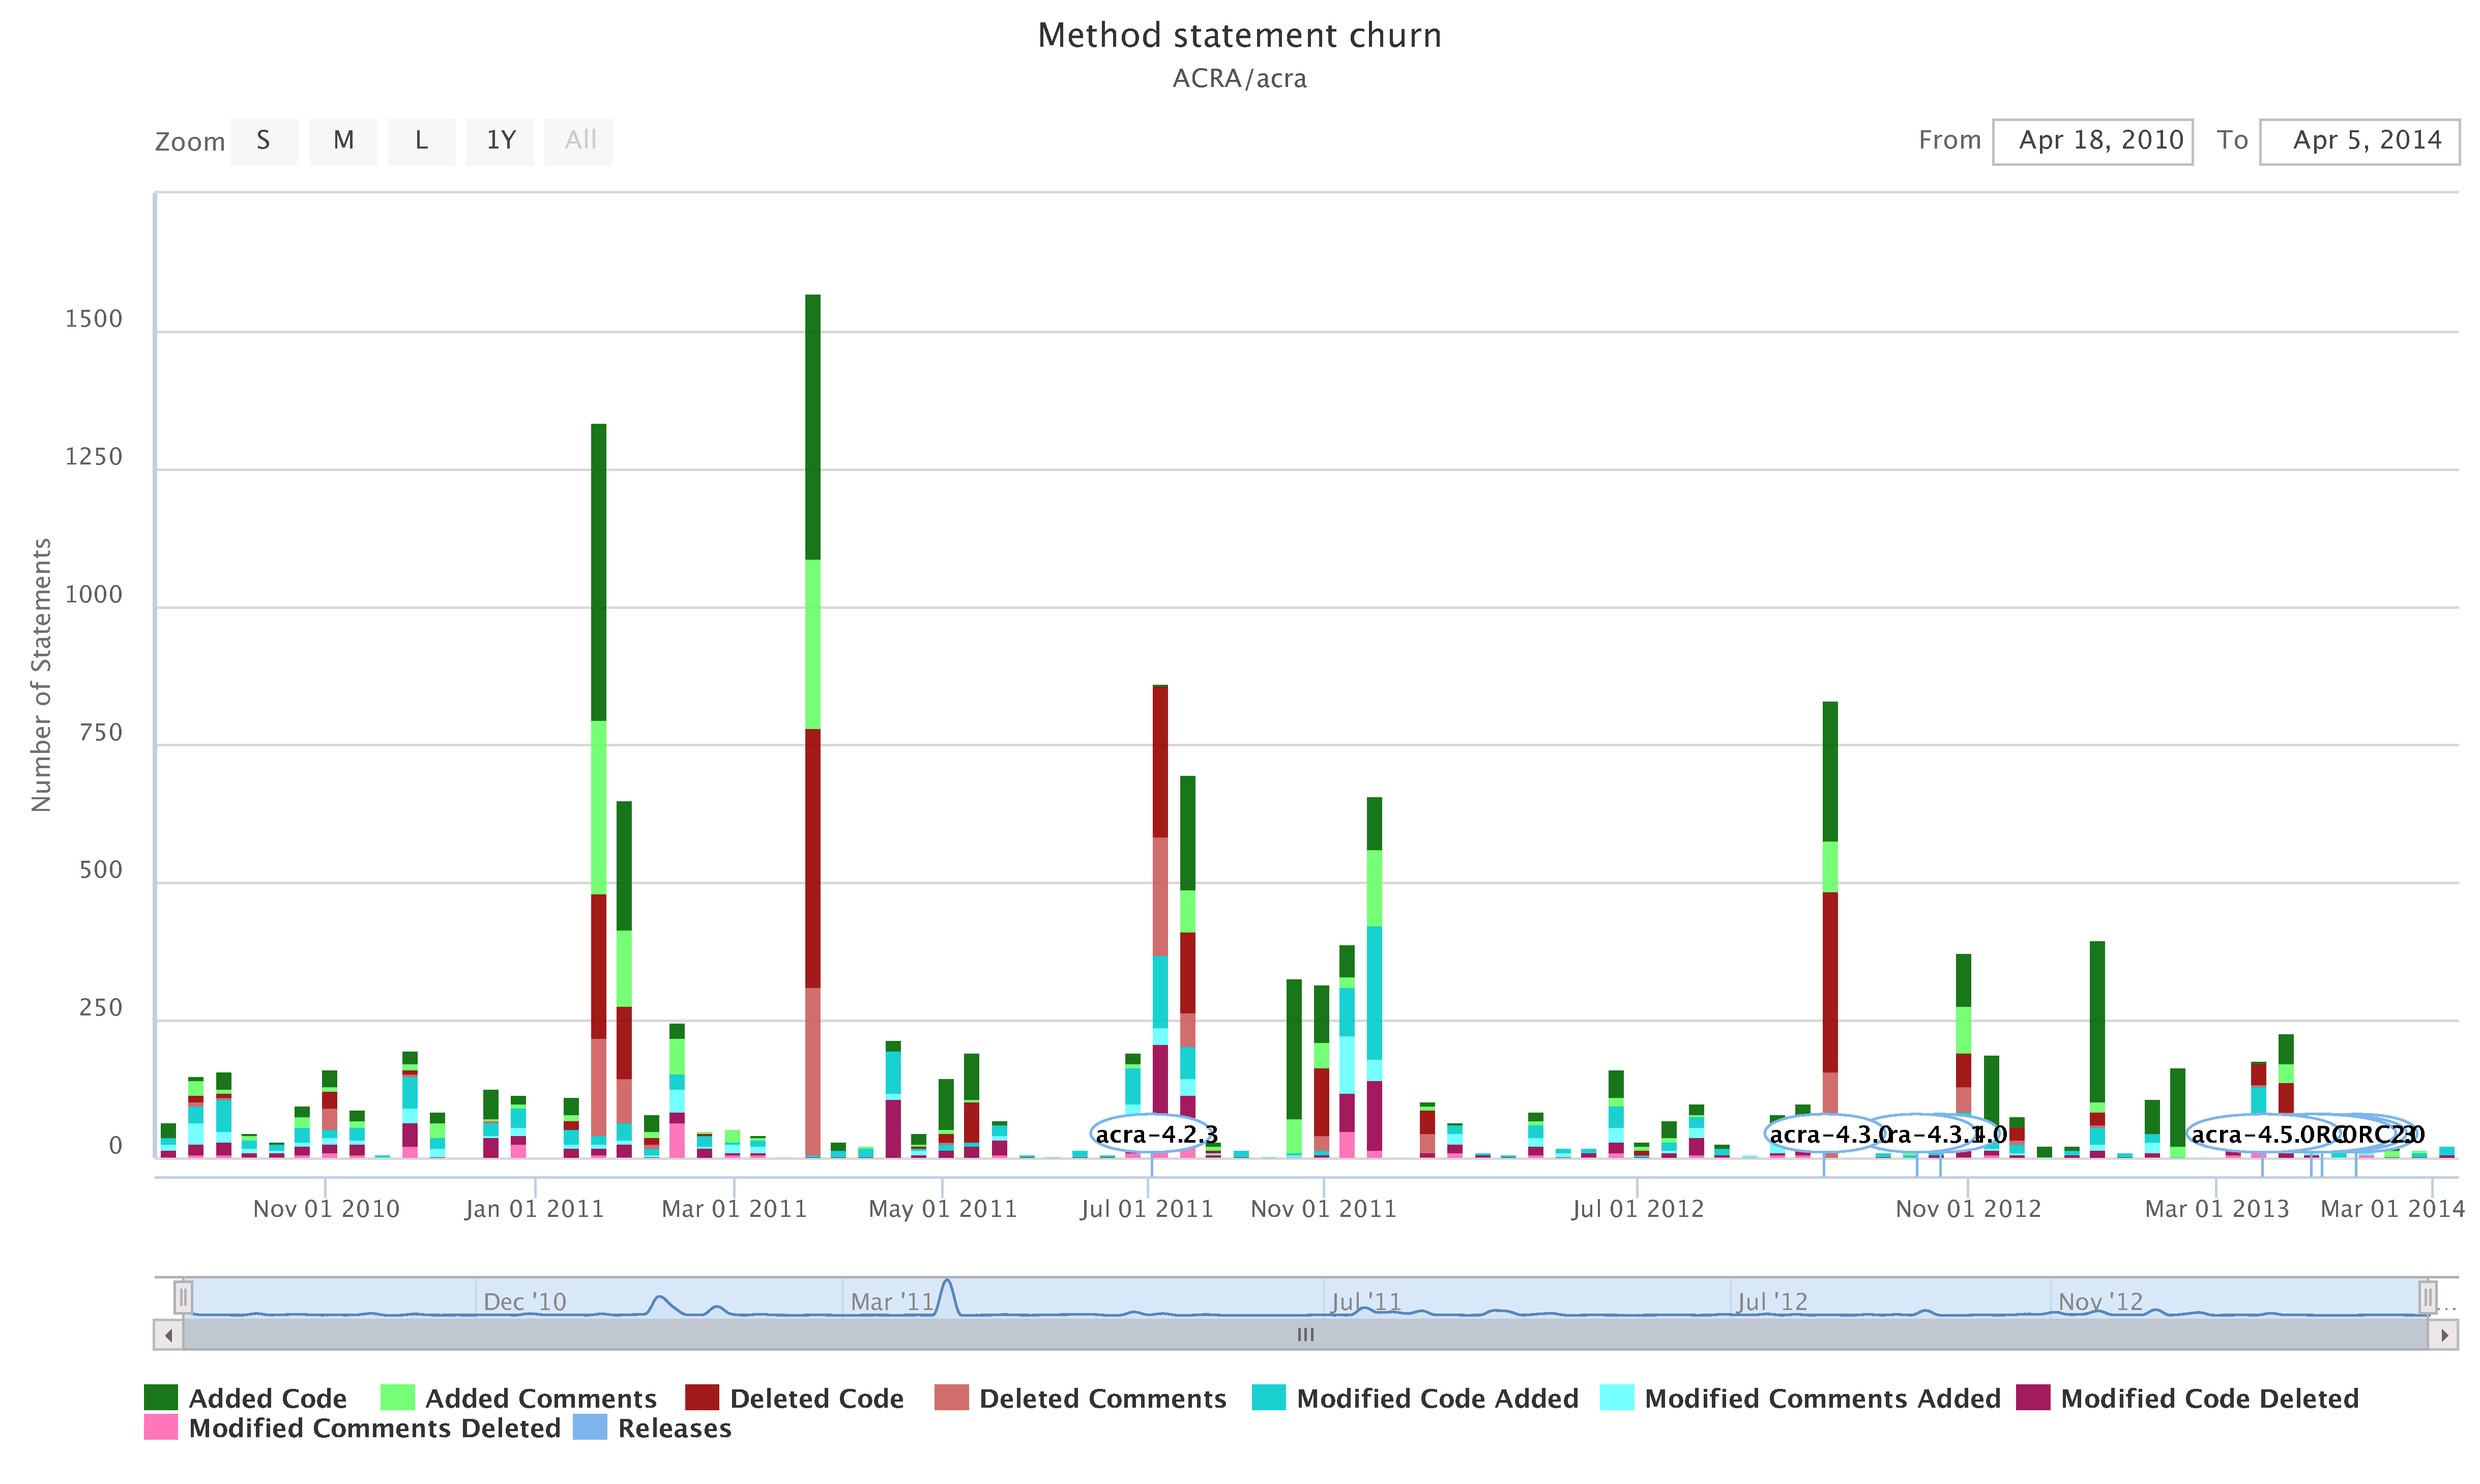
\includegraphics[width=1.5\textwidth]{images/statement_visual_acra}
%     \caption{Method Statement Change Visualization for acra}
%     \label{fig:statement_visual_acra}
%  \end{figure}
% \end{landscape}

% TODO talk about each of them specifically
\begin{landscape}
\thispagestyle{empty}
 \begin{figure}
  \centering
        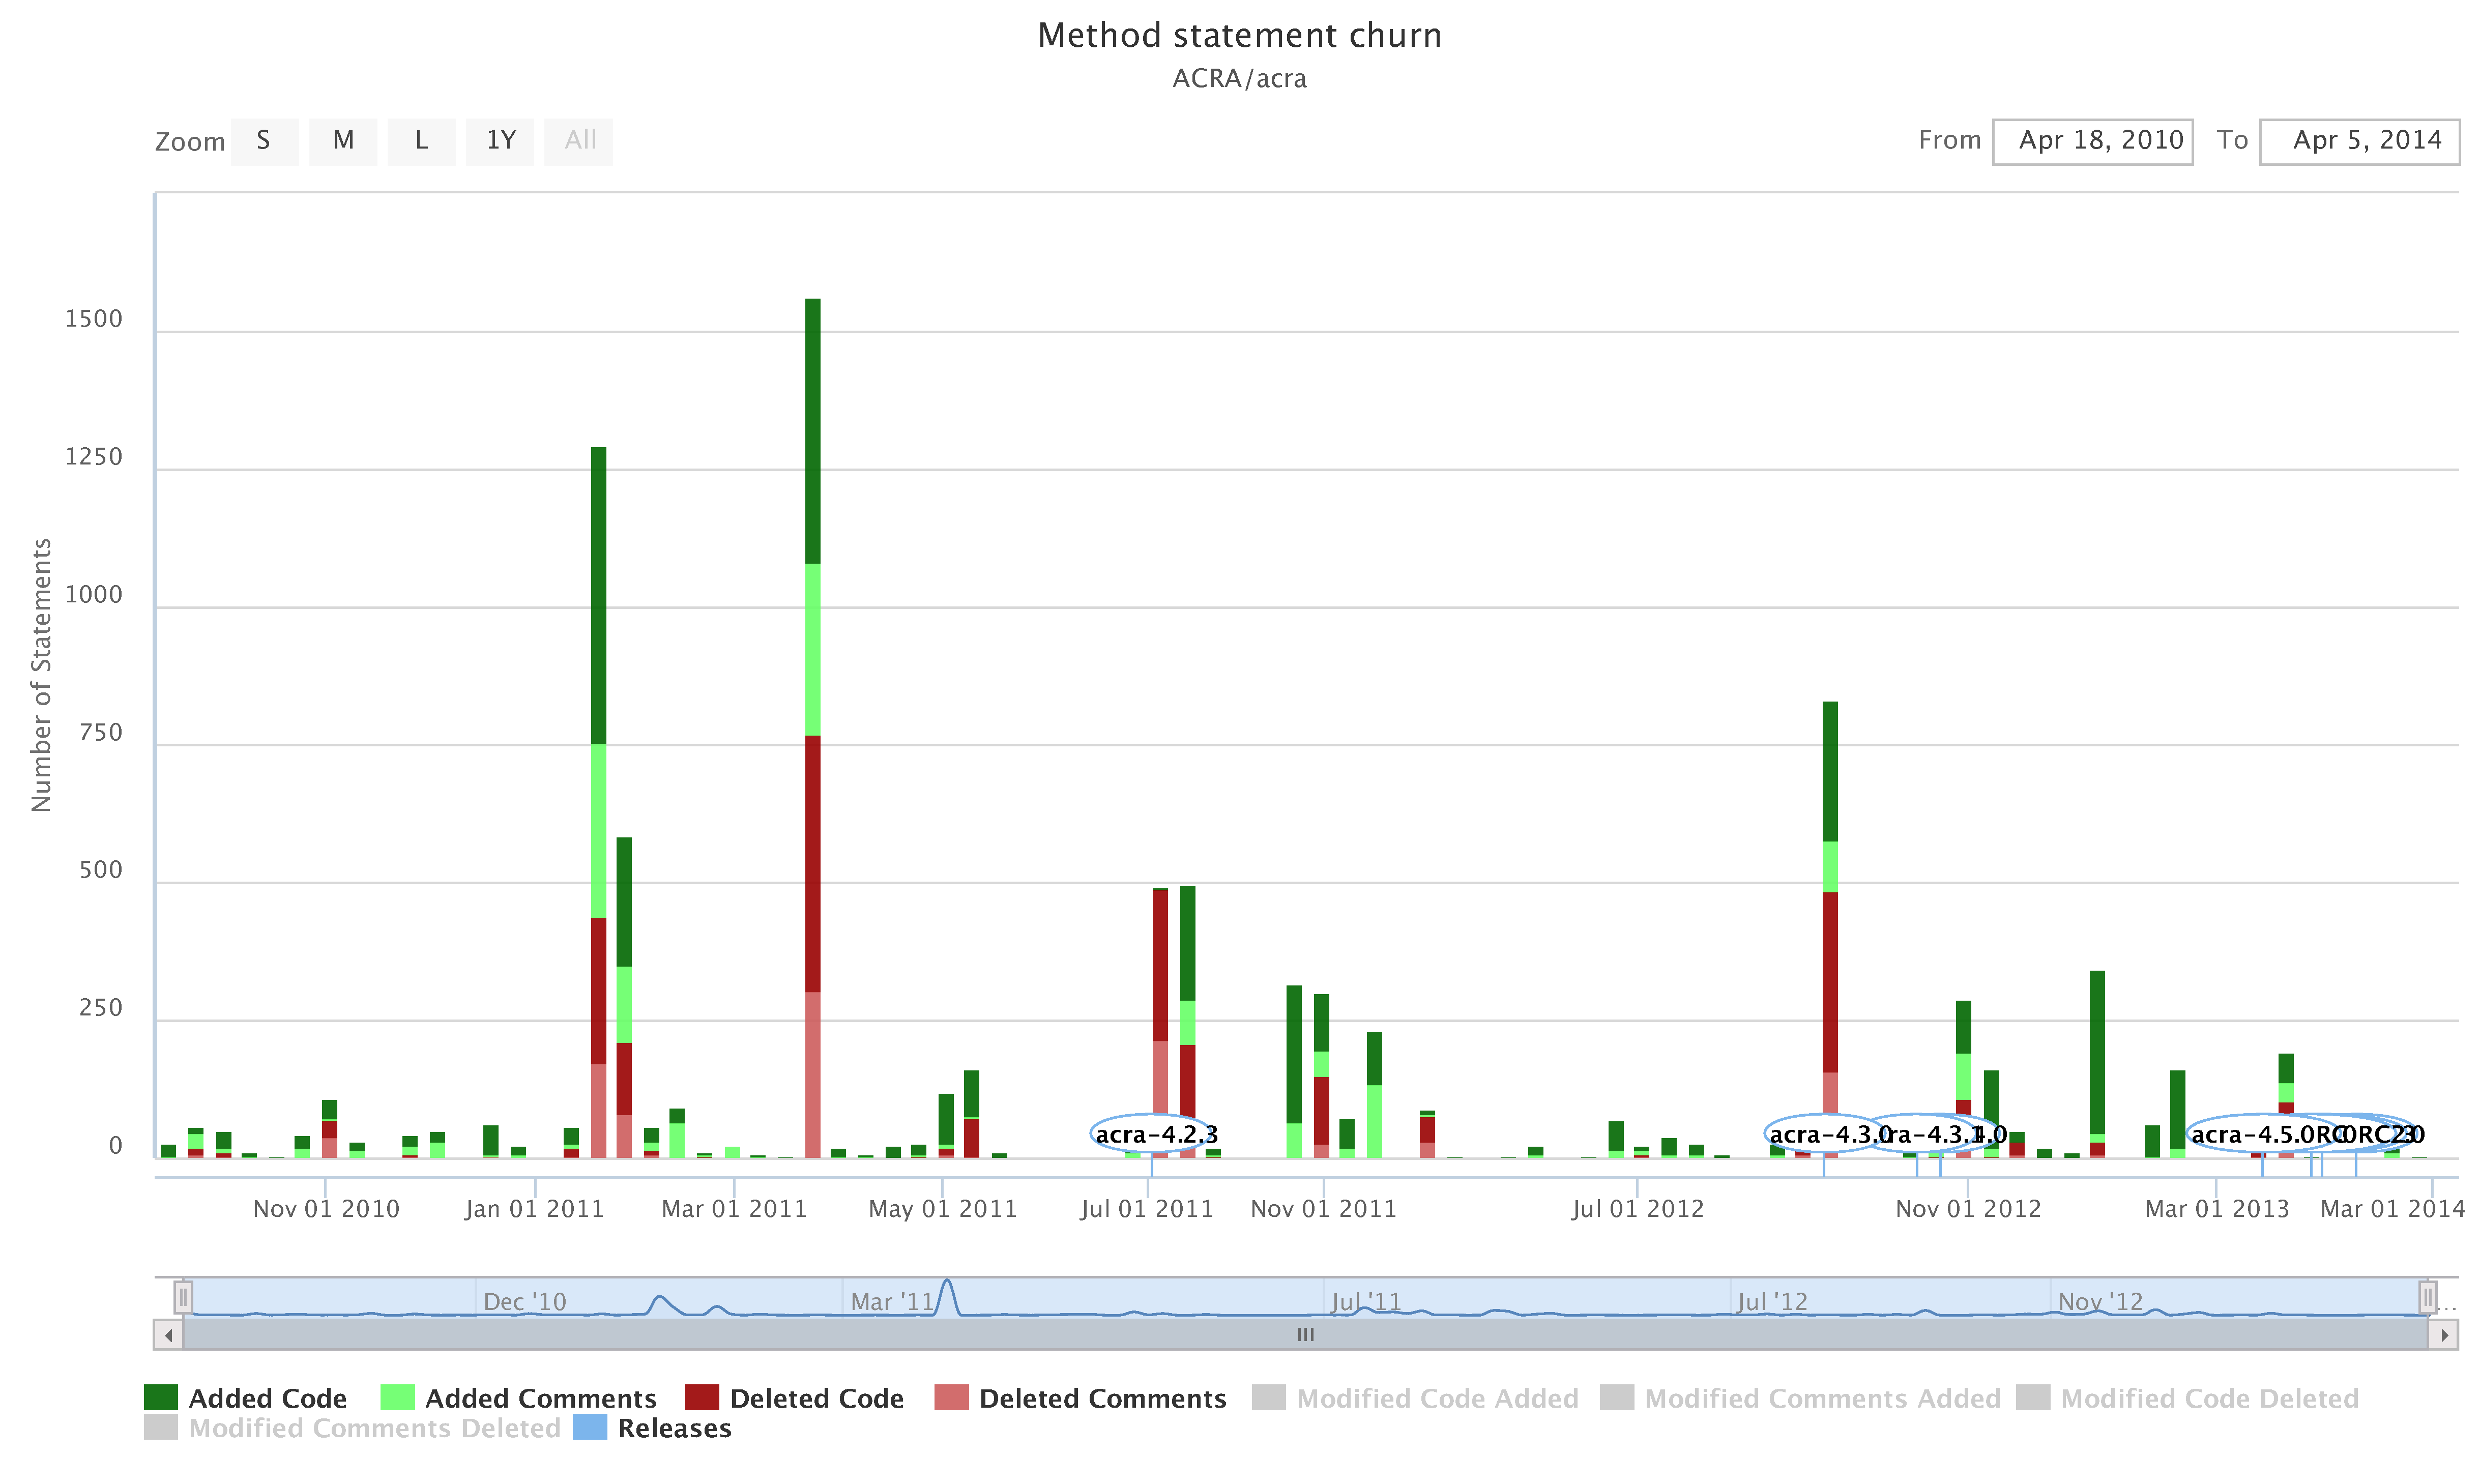
\includegraphics[width=1.5\textwidth]{images/statement_add_delete}
    \caption{Method Statement Added \& Deleted Visualization for acra}
    \label{fig:statement_add_delete_visual_acra}
 \end{figure}
\end{landscape}
\thispagestyle{plain}

\begin{landscape}
\thispagestyle{empty}
 \begin{figure}
  \centering
        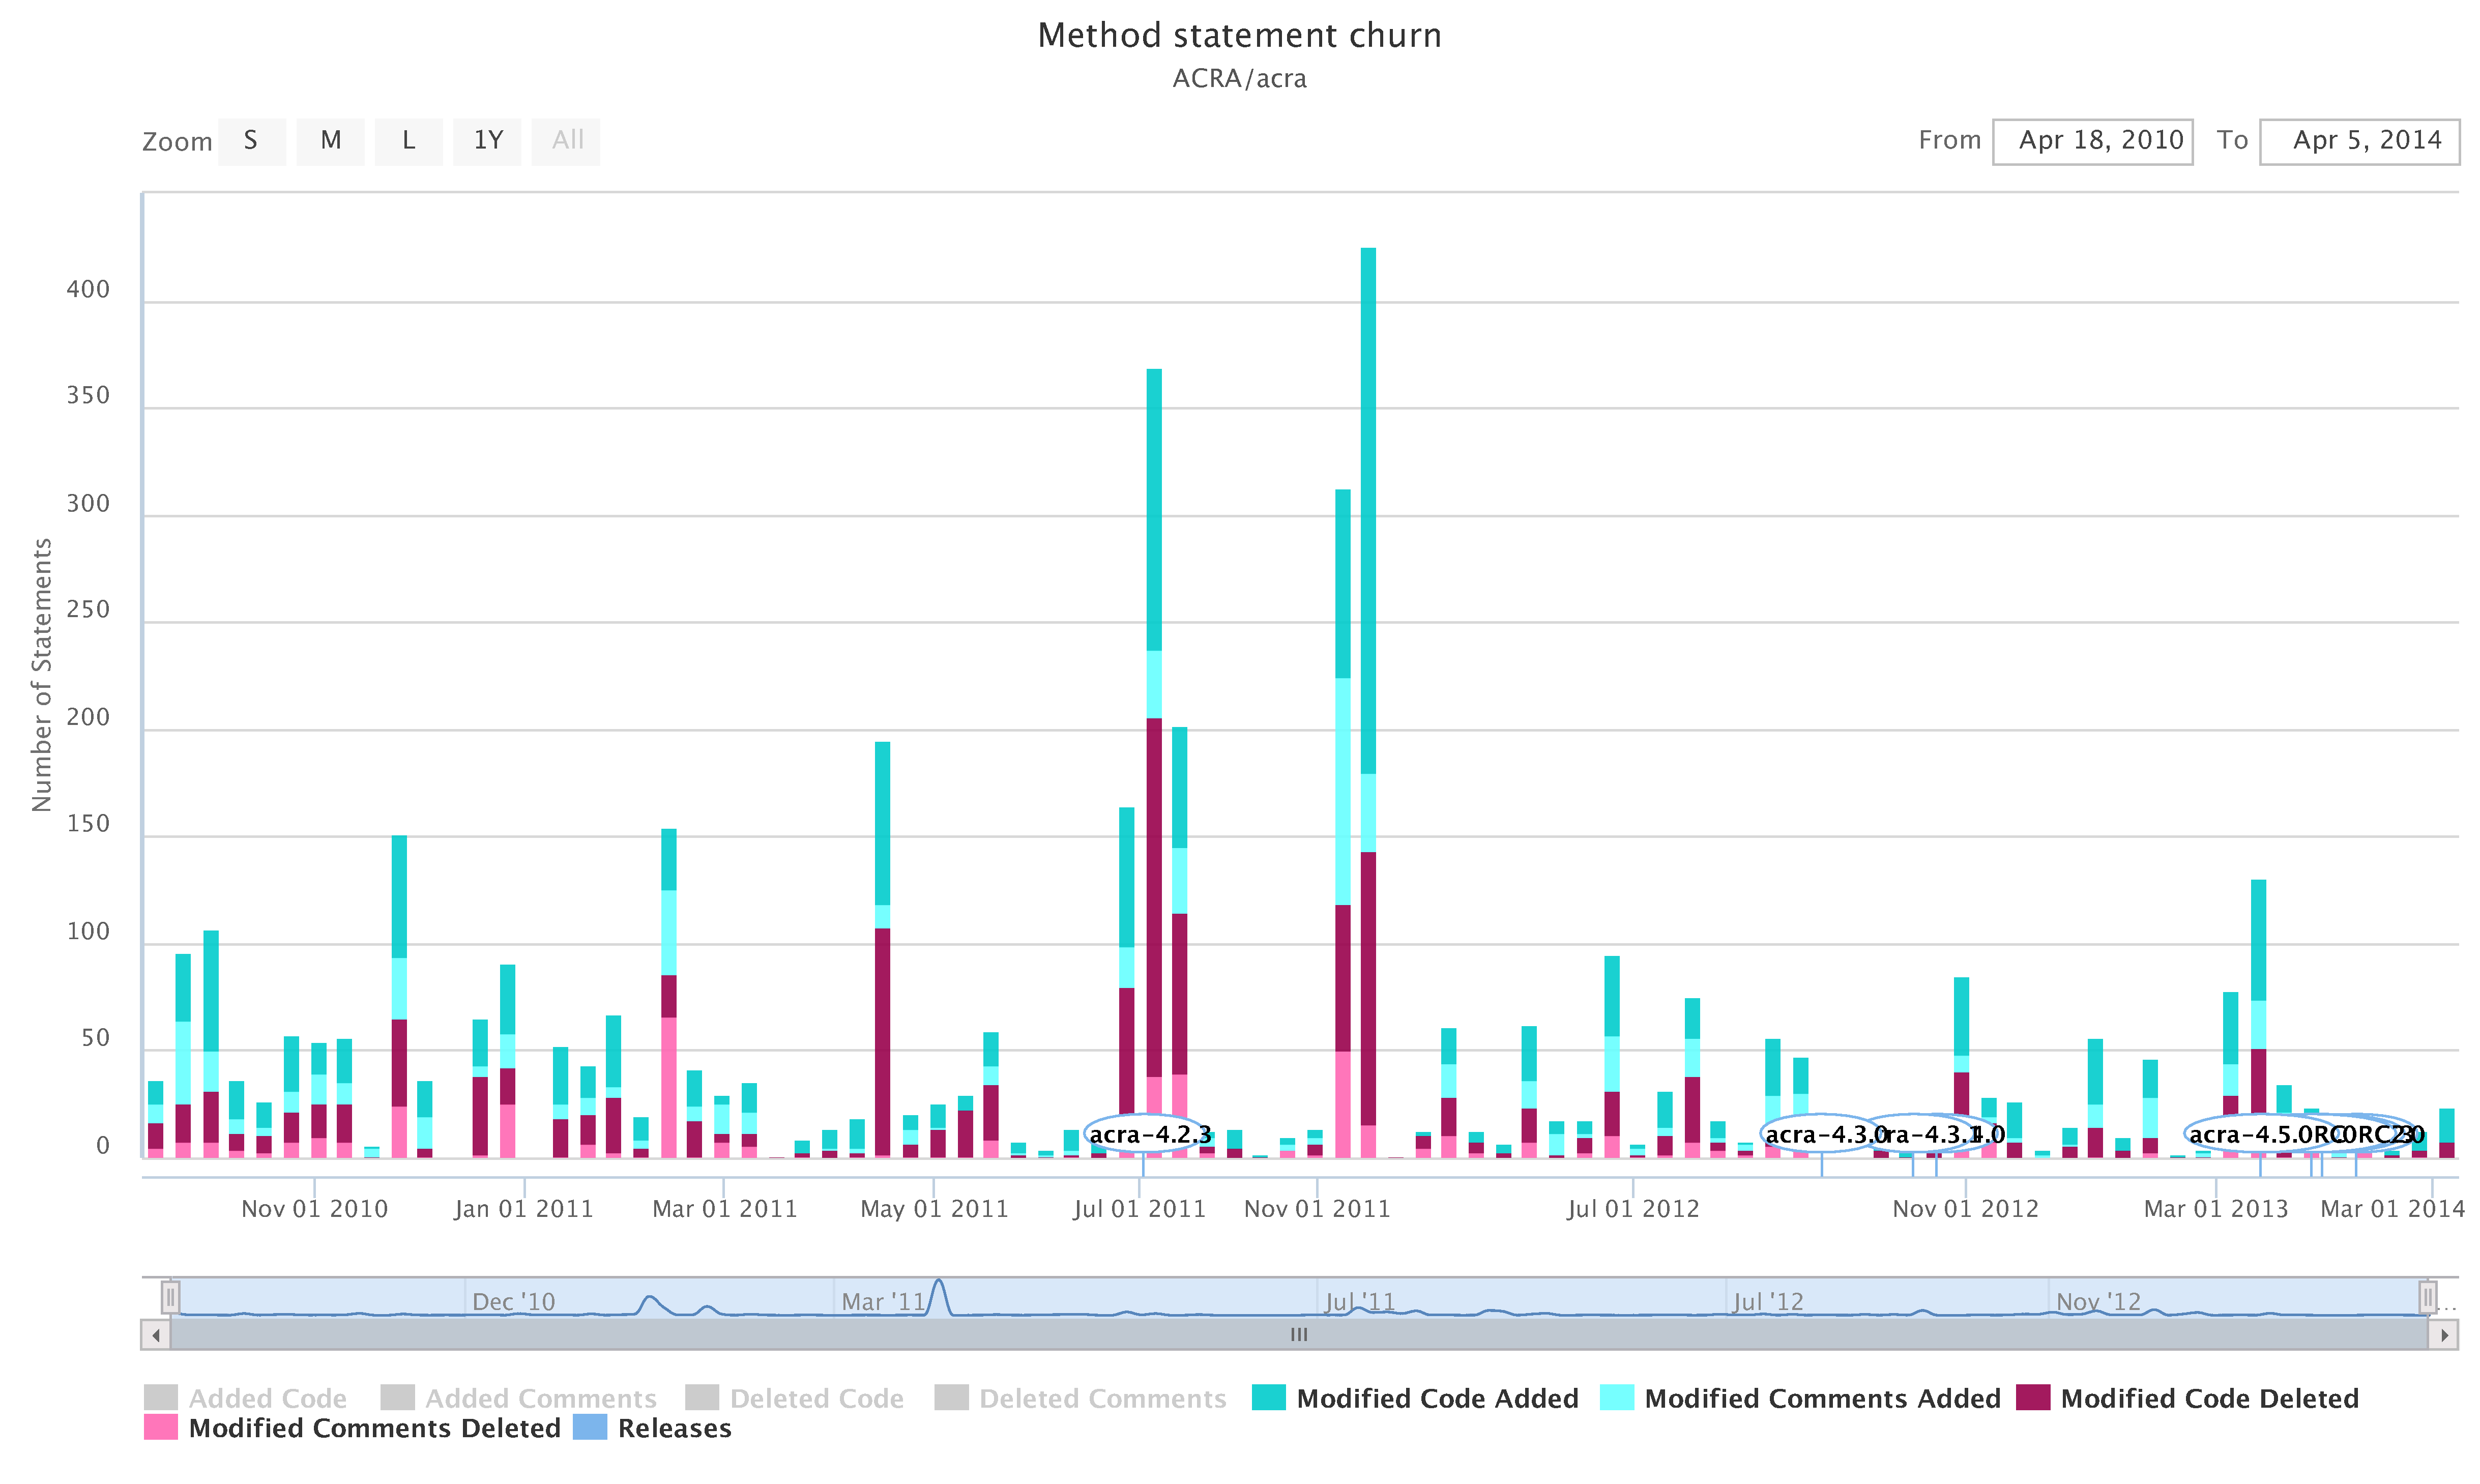
\includegraphics[width=1.5\textwidth]{images/statement_modified}
    \caption{Method Statement Modification Visualization for acra}
    \label{fig:statement_modified_visual_acra}
 \end{figure}
\end{landscape}
\thispagestyle{plain}

% Decided whether to keep the other names or update them to these ones (on the site as well).
%So finally we have the categories: \textit{Modified Code Addition}, \textit{Modified Comment Addition}, \textit{Modified Code Deletion} and \textit{Modified Comment Deletion}.
\chapter{Prediction with Commit Data}
\label{chap:prediction}

% TODO discuss research question **************************************************************************************************

% How the visualization helped 	
The visualization for the data collected from the projects helps provide several insights into data set which can used to help with the creation of the prediction scheme. With the data visualized, a more general look of the data collected is available. While creating the method for predicting change within the project the visualizations provided a helpful resource. The visualization can help identify relationships between variables and general trends. The actual data used for training the prediction model is outlined in \autoref{sec:prediction_data}. After that the prediction model is detailed in \autoref{sec:prediction_method}. %Finally, the actual implementation is discussed in \autoref{sec:implementation}

The data presented in the visualization is used towards creating an approach to predict whether a method will change within the next five commits. The machine learning algorithms used in the approach are \gls{svm} and \gls{rf}. Of course the performance of a prediction method will be influenced by several factors including; the size of the sample, the features used for training and balancing of the data set.

\section{Prediction Data}
\label{sec:prediction_data}

The data used to predict changes within a project is originally from the visualizations. For more information about the specific information collected see \autoref{sec:collection}, \autoref{sec:storage} and \autoref{sec:parsing}. The commit data collected from the target \gls{oss} project is used to make predictions. The goal is to predict whether a method within a project will change within the next five commits. As outlined in \autoref{sec:parsing}, the different types of changes can be either additions, deletions, modifications or no change at all.

The machine learning model requires samples from the data set to train from which allows for predictions of new elements. The training samples taken must also be categorized based on the desired outcome of the machine learning algorithm. This requirement provides some restrictions on which values can be included in the sampling. Since the categorization is whether a method will change, all methods sampled need to be able to collect data the next five commits following the current commit. Therefore methods that are within the last five commits of the training sample window are not included in the training set for the data model.

\begin{figure}[!ht]
    \centering
        %Generated from http://jsfiddle.net/u43dfLxp/1/
        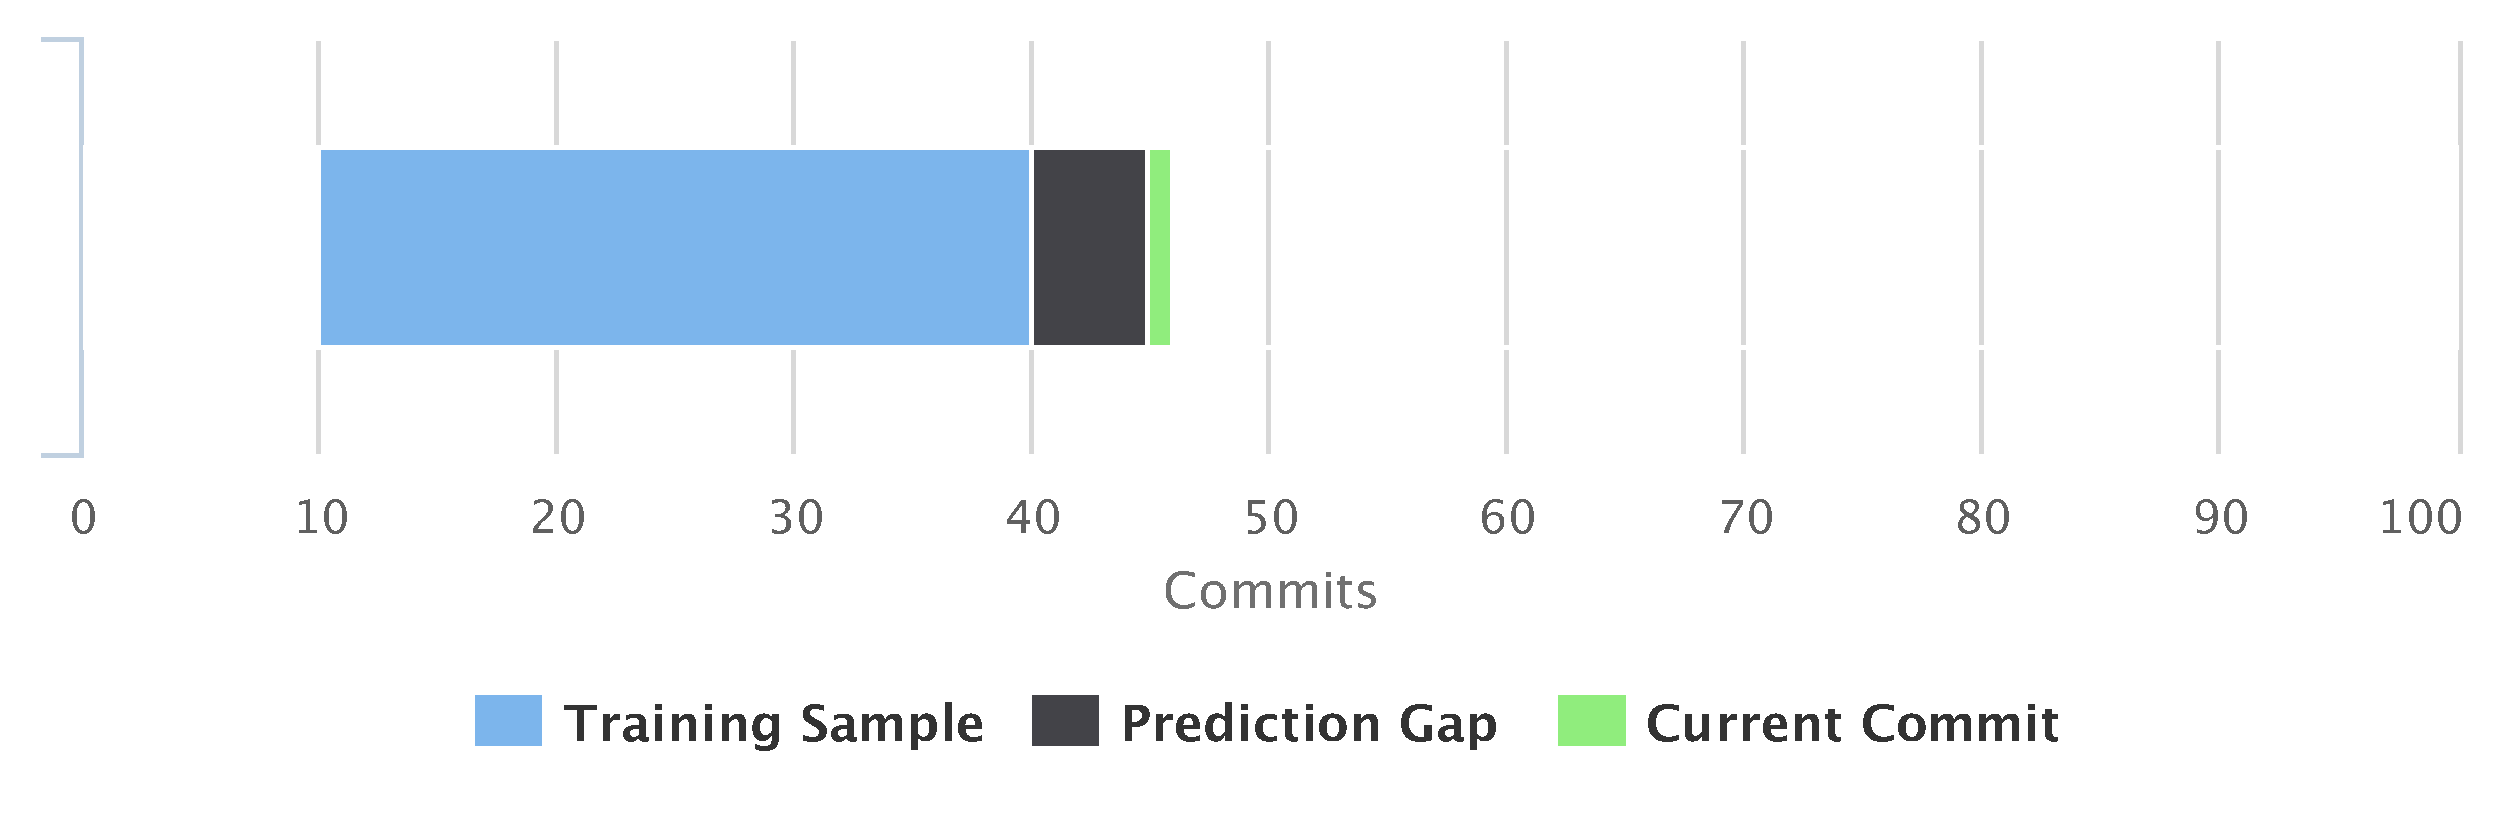
\includegraphics[width=1.0\textwidth]{images/training_sampling}
    \caption{Training Sampling Layout}
    \label{fig:training_data_range}
\end{figure}

As noted above one of the key factors in the performance of the prediction approach is the size of the sample set. The sample set size is restricted by a variable value \gls{swr} which controls the number of commits considered for sampling from. The data will only be sampled within a limited range of commits as outlined in \autoref{fig:training_data_range}. In this case, the \gls{swr} is 30 and the prediction gap is 5. The prediction gap takes into account the categorization restriction, preventing sampling from the last five commits.

Another consideration when sampling the data is the distribution of the categories. Most of the time, a data set will contain more samples in one category than the other. For example, a sample may contain $80\%$ methods with no change within the next five commits and $20\%$ methods with change. Ideally the number of methods with changes and without changes in the next five commits would be close to $50\%$. When the distribution of samples for each category is very close the model will often perform better. However in cases were the data is highly skewed to one classification over the other the model will often predict the larger classification for input values. \gls{os} will take more samples (duplicates) from the smaller classification reduce the difference in size with the larger classification. Alternatively, undersampling the data set will use remove samples from the larger classification reduce the difference in size with the smaller classification.

% Discussed further in section in approach
Undersampling is applied to a data set by measuring the number of samples that are in each category. The larger of the two is reduced by discarding samples at random until the data set is the same size as the smaller data set. This will reduce the number of samples used to train the model and may reduce the performance of the model based on the decreased number of samples. In cases where there are a limited number of samples for the smaller category undersampling may not be ideal. \gls{os} alternatively increases the number of samples by calculating the number of samples in each category and expanding the smaller category by re-sampling values from the data set until both categories are equal in size. Both approaches can be used together so that the smaller category is expanded to at most twice it's original size. If the initially smaller category is still smaller, the larger category set is reduced to the size of the smaller category. When selecting values for re-sampling or removal the selection process is random to ensure the distribution of the data is preserved. For example, if category $a$, with $|a| = 100$ and category $b$ with $|b| = 1000$. \gls{os} will be applied to category $a$ since $|a| < |b|$. Therefore $a$ will apply random re-sampled until $|a_n| = |a| \times 2$ or $|a_n| = |b|$. Once one of the conditions is met \gls{os} is complete. Next undersampling is applied to the larger category $b$, were samples are randomly removed from $b$ until $|b_n| = |a_n|$.

% Discuss the percentage of sampling.
Once the categories are balanced then the model can use the data. However with large sample sizes a reduction of the sample set may be necessary. The variable $sample_r$ is the percentage of the number of samples taken from the range. Instead of picking an arbitrary number of samples, a ratio was used to scale the number of samples taken based on the size number of available samples. When sampling if the ratio is at $50\%$ then only half of the values retrieved will be used to train or test. For some of the larger data sets sampling $100\%$ of the data from the range would take a lot longer. Therefore sampling a percentage of the data set is commonly used to decrease the training time. In order to provide a more stable model a random sample of the sample range is used so that each data entry in the sample has the same chance to be within the training or test data set. Using the example from above, $a$ and $b$ have been oversampled and undersampled such that their new size is represented by $|a_n|$ and $|b_n|$ respectively. Given that a sample ratio of $50\%$ is used then both sets $a$ and $b$ would be reduced by the ratio by randomly sampling from each set to create new sets. The size of each set would be $|a_n| \times r$ where $r$ is the ratio value.

%238, ReportField.java            |           8234 | public boolean getValue() {                                                                          |           0 | william-ferguson-au |  0.0464135021097046 | ("{3,3,0,0,0}","{68,1816,549469,779372,208198}")                              |        0
\begin{table}
\begin{center}
    \begin{tabularx}{\linewidth}{|l|X|l|l|}
        \hline
        Feature & Description & Data & Example \\
         & & & Vector \\
        \hline
        Com & The individual who committed the change & bob & 5 \\ \hline
        Name & The name of the file & Main.java & 3 \\ \hline
        Sig & The method signature related to the change details & void getValue() & 46\\ \hline
        %$change_i$ & Whether the method changed or not at the current commit & 3 & 1 \\ \h$f_{\Delta}$line
        
        $f_{\Delta}$ & The frequency that the method is changed within the \gls{swr} & 0.0464 & 0.0464 \\ \hline
        $sf_{\Delta}$ & The frequency that the method is changed within the last 10 commits.  & 0.1 & 0.1 \\ \hline
        $t_\Delta$ & The time between the current commit $c_i$ and the previous commit $c_{i-1}$ & 2148 & 2148 \\ \hline

        Length & The length of the method in this commit & 10 & 10 \\ \hline
        $change_{t-1}$ & Whether a change has occurred in the previous 5 commits & $\{3, 0, 0, 3, 0\}$ & 1 \\
        \hline
        $change_{t}$ & Identifies whether a change occurred within the next 5 commits for the given method & 0 & 0\\
        \hline
    \end{tabularx}
\end{center}
    \caption{Candidate features for \gls{svm} model}
    \label{tab:candidate_features}
\end{table}

% Name => Methods within a file are likely going to have similar change patterns
% Signature => A method change history will likely be unique
% Change_i => Whether the method changed or not at the current commit may provide insight as to whether the next 5 commits will feature a change as well.
% committer => Users may change in different change patterns thus helping identify whether this will be a change or not, 
% freq_change => Helps identify how likely the file is to change

The \autoref{tab:candidate_features} outlines each feature used for training the prediction model. An example of each feature is provided to further illustrate the feature. As stated in the previous \autoref{subsec:svm_prediction}, the values need to be processed into a usable format for \gls{svm} or \gls{rf}. First the data is extracted from the database as \textit{raw} values as shown in the \textit{\textbf{Data}} column. Text values are mapped to a integer value. For example the \textit{Name} value, ``Main.java'' will be mapped to the value 3. The reason the value is 3 is because 2 other methods have already been mapped and therefore method name is mapped to the next available mapping. Similarly both \textit{Com} and \textit{Sig} will be mapped from their respective values ``void getValue()'' and ``bob'' to 46 and 5. Numerical values are converted by casting the value to a floating point value if the value is not that type already. For spacing reasons all the values in the table that were integers to begin are shown without a ``.0'' following.
%converted into floating point numbers.

Another small change made to the data to create a vector for the prediction model was to convert the change type into a change indicator vector using \autoref{eq:change_type}. The vector is converted into a single value which indicates whether a change has occurred in the previous five commits. This process is done through calculating the sum of the change vector using \autoref{eq:change_reduce}. Finally, the change indicator, $change{i-1}$, is identified using \autoref{eq:change_prev}.

\begin{equation} 
\label{eq:change_type}
C = \left\{\begin{matrix}
1 & \text{if} change > 0 \\
0 & \text{otherwise}
\end{matrix}\right.
\end{equation}

\begin{equation} 
\label{eq:change_reduce}
reduce = \sum_{i=t-5}^{t}{c_i}
\end{equation}

\begin{equation} 
\label{eq:change_prev}
P = \left\{\begin{matrix}
1 & \text{if} reduce > 0 \\
0 & \text{otherwise}
\end{matrix}\right.
\end{equation}

$f_{\Delta}$ is calculated by taking the number commits in which involve changes to the current method ($c_i$) within the \gls{swr} divided by the current number of commits ($c_{cur}$) since the start of the \gls{swr}. This is formalized in \autoref{eq:freq_change}. A frequency of change is available for the duration of the \gls{swr}.

\begin{equation}
\label{eq:freq_change}
f_{\Delta} = \frac{|c_i|}{|c_{cur}|}
\end{equation}

$sf_{\Delta}$ is calculated by reducing the range sampled to $s$. Then counting the number of times the method changes within the last $s$ commits and dividing it by $s$. The size of the short frequency can be any value that is less than the size of the \gls{swr}. For use in the rest of the paper $s = 10$ which means that the $sf_{\Delta}$ is for the last $10$ commits.

%Both $change_{prev}$ and $\Delta t$ are actually each 5 features since they are a set of features. $change_{prev}$ shows the type of change that occurred for the last 5 commits. Similarly 

$t_\Delta$ is the difference between the current commit time ($t(c_i)$) and the previous commit time ($t(c_{i-1})$) calculated in \autoref{eq:time_delta}. For the feature only the latest time difference is used.

\begin{equation}
\label{eq:time_delta}
\Delta t_{i} = t(c_i) - t(c_{i-1}), i > 1
\end{equation}

\section{Prediction Method}
\label{sec:prediction_method}

% TODO talk about the machine learning algorithms more specifically:
% - Which are we using
% - Why did we choose them
% - what parameters they use
	% - What we set those parameters to
	% - and why

For this approach a machine learning algorithm is used to create a prediction model. The data used to train the model is collected as shown in \autoref{sec:prediction_data}. The machine learning algorithms that can be used are either \gls{svm} or \gls{rf}. Each of these method are widely used for data mining techniques and are easy to use. 

% TODO talk about how to set up the predictions for use (actual implementation)
	% - including what to expect from the approach and so on.
The \gls{svm} model was created through the use of a libsvm\footnote{\url{https://www.csie.ntu.edu.tw/~cjlin/libsvm/}} binding for ruby, rb-libsvm\footnote{\url{https://github.com/febeling/rb-libsvm}}. This library was a good fit since the data was collected using a ruby script. For \gls{rf} python library scikit-learn\footnote{\url{http://scikit-learn.org/stable/}} was used. The reason for using python rather than ruby, was a lack of mature library for \gls{rf} in ruby.

The method for using the approach would be to collect the data from the project. Once the data is collected the prediction model can be created through a sampling a training set. Once the model is trained predictions can be made using the model on new data. The next chapters puts the approach into practice by training the model and testing the model using subsets of a project data set.
\chapter{Experiments}
\label{chap:experiments}

\section{Experimental Project Data}
\label{sec:experimental_project_data}

One thing that should be noted for the experiments that were run. Since all of the data was known before the model was even created artificial cut off dates were created to allow for the feature set to be tested as to their effect on the model. A test project, acra (developed by the user ACRA), was chosen to develop the method on. 

%The project data was extracted from GitHub from when the project was initially committed to GitHub (2010-04-18 15:52:18-04) till the cut off day of extraction (2015-06-05 09:02:56-04). The cut off day was the day the data was extracted from GitHub and after of which the data analysis was initiated.

% TODO consider placing this into introduction
\begin{table}[h!]
\begin{minipage}{\textwidth}
\begin{center}
    \begin{tabular}{|c|c|c|c|c|c|}
        \hline
        Owner & Project & Start Date & End Date & \# of & \# of \\
         & & & & Commits & Developers \\
        \hline
        ACRA & acra\footnote{\url{https://github.com/ACRA/acra}} & 2010-04-18 & 2015-06-05 & 404 & 32 \\
        apache & storm\footnote{\url{https://github.com/apache/storm}} & 2011-09-16 & 2015-12-28 & 2445 & 261 \\
        facebook & fresco\footnote{\url{https://github.com/facebook/fresco}} & 2015-03-26 & 2015-10-30 & 313 & 47 \\
        square & dagger\footnote{\url{https://github.com/square/dagger}} & 2012-06-25 & 2016-01-30 & 496 & 39 \\
        deeplearning4j & deeplearning4j\footnote{\url{https://github.com/deeplearning4j/deeplearning4j}} & 2013-11-27 & 2016-02-13 & 3523 & 62 \\
        \hline
    \end{tabular}
\end{center}
\caption{Experiment projects}
\label{tab:project_summary}
\end{minipage}
\end{table}

The complete list of projects that were tested is found in \autoref{tab:project_summary}. The number of commits excludes any commit that lacked a change to a file containing Java code. Since the primary interest was to parse Java code, files containing Java code were used while all other files are ignored. These measures provide a more accurate description of the project in terms of the analysis and predictions made on it. Secondly, the number of developers does not map effectively to what git uses as committers and authors. Instead, the number of developers includes all individuals (removing duplicates) who committed or authored commits to the current project.

%TODO place the tables in better positions.
\begin{table}
\begin{center}
    \begin{tabular}{|c|c|c|c|c|c|}
        \hline
        Project & \# of Methods & \# of Methods & Avg \# of & Avg \# of Methods \\
         & & Changes & Commits / Year & Change / Commit \\
        \hline
        acra & 1309 & 3605 & 67.33 & 9.51 \\
        storm & 14599 & 50037 & 489 & 24.03 \\
        fresco & 3463 & 4139 & 313 & 14.73 \\
        dagger & 1827 & 6314 & 99.2 & 13.70 \\
        deeplearning4j & 29896 & 82198 & 880.75 & 24.33 \\
        \hline
    \end{tabular}
\end{center}
\caption{Project Change Statistics}
\label{tab:project_stats}
\end{table}

Each of the projects selected on GitHub using the list of Java projects with a large amount of contributions. Open source projects were targeted to simplify any usage concerns. Therefore in order to be selected the program had to clearly use an \gls{oss} license. Secondly, the program also needed to have at least a 6 months worth of development and at least 300 commits to provide a large enough dataset to analyze. An effort was also made to pick projects of different sizes to provide better tests of various conditions.

The first project acra is a Android bug logging tool used with Android applications to capture information related to bugs or crashes. The information is sent to the developers to help them address the issues that their clients encounter while using there application. The second project, apache's storm, real time computational system for continuous streams of data. This project is one of the larger projects and has a large development community. The third project, facebook's fresco, is the smallest project with the shortest development period. This project provides a library for using images on Android to attempt to solve limited memory issues with mobile devices. The fourth project, square's dagger, is a Java application used to satisfy dependencies for classes to replace the factory model of development. The final project, deeplearning4j, is a distributed neural network library that integrates Hadoop and Spark. This application is the largest of the 5 projects and provides a large wealth of data to analyze.

\begin{table}
\begin{center}
    \begin{tabular}{|c|c|c|c|c|c|}
        \hline
        Project & Avg \# of & Avg \# of & Avg \# of & Max & Min \\
         & Methods Change & Changes & Commits / & Commits & Commits \\
         & / Year & / Method & Developer & / Year & / Year \\
        \hline
        acra & 600.83 & 4.52 & 13.93 & 119 & 33 \\
        storm & 10007.4 & 5.93 & 15.47 & 948 & 118 \\
        fresco & 4139 & 1.49 & 156.5 & 313 & 313 \\
        dagger & 1578.5 & 5.64 & 16 & 236 & 4 \\
        deeplearning4j & 20549.5 & 5.69 & 65.24 & 2018 & 65 \\
        \hline
    \end{tabular}
\end{center}
\caption{Project Change Statistics 2}
\label{tab:project_stats_2}
\end{table}

In order to get a more detailed understand of the selected projects numerous measures were taken. These measures also allow for each projects to be compared to each other in terms of the development of each of the projects. The size of the project is represented through number of commits, methods. The size of the development team is also provided. The length of each project is shown and most of the measures average on a yearly term.

% TODO reference the table
Several average measures were also taken which detail the amount of change that occurs within the project. The average number of commits per project coupled with the average number of changes per commit clearly indicates the amount of changes that are occurring with in the project. The rate at which methods are change provides good insight into the growth of a project. While some changes may involve the addition of new methods, others may include the removal of methods or the modification of methods. The other measures relating to the amount of change occurring with a project on average are the number of methods changed per year and the number of changes per method. Each of these further outline how the changes are being made to the project on average.

A few of the measures are related to the number of developers. These while provided are not the primary focus. The information provided by tracking developer interactions with each other or the repository could be integrated into future work.

\begin{table}
\begin{center}
    \begin{tabular}{|c|c|c|c|c|c|c|}
        \hline
        Project & Max \# of & Min \# of & Max \# of & Min \# of & Max \# of & Min \# of \\
         & Methods & Methods & Change / & Change / & Commits / & Commits / \\
         & Changed & Changed & Method & Method & Developer & Developer \\
         & / Year & / Year & & & & \\
        \hline
        acra & 1503 & 183 & 52 & 1 & 229 & 1 \\
        storm & 26526 & 2152 & 314 & 1 & 622 & 1\\
        fresco & 4139 & 4139 & 33 & 1 & 269 & 44 \\
        dagger & 3374 & 171 & 65 & 1 & 157 & 1 \\
        deeplearning4j & 35869 & 4377 & 345 & 1 & 1987 & 1 \\
        \hline
    \end{tabular}
\end{center}
\caption{Project Change Statistics 3}
\label{tab:project_stats_3}
\end{table}

While the purposed method was being developed ACRA's acra project was primarily used for exploring and initial testing of the approach. After experimenting on acra a few of the potential candidate feature sets were distinguished based on their superior performance. Experiments were then run on other projects using the feature sets that performed better.

    % An effort was made to not count individuals twice however some users may have changed their user name and thus showed up several times.
% NOTE the number of commits is the number of commits that contained Java code and thus was useful towards parsing.
% Note the number of developers is the total number of developers who both committed or authored commits, aka people who made pull requests are included.

% TODO merge the different experiment notes sections into one subsection

% \subsection{Experiment 1}

% % TODO look for test results for this one
% The first set of experiments were preliminary and used \gls{svm} as the approach for prediction algorithm. They attempted to predict whether a given method would change within the next 6 commits. The test was done one using ACRA's acra (hence forth just called \textit{acra}). The data set was divided into four sections based on the date length. So each section of the data was the project's lifespan divided by 4 long. The sampling method from the data set $data_i$ was to use the first $n$ tuples ordered by date. The value of $n$ was tested at 100 and 1000. The data set $data_i$ contained tuples which had changes and ones that had no changes.

% $|data_i| = \frac{|date_f - date_s|}{4}$

% The results of these experiments were not particularly promising scoring accuracy, precision, recall and recall around $50\%$ or below. The experiment was run such that $data_i$ would be used for training and $data_{i+1}$ would be used for testing. For example $data_1$ would be used to train $model_{1,2}$ and $data_2$ would be used to test the $model_{1,2}$. A slight variation was also tested where $data_i$ trained $model_i$ and was tested use each data set $data_j$ that had $j > i$. This however still provided poor results similar to the original experiment. \autoref{fig:exp_1_data_range} shows how the data is distributed.

% % TODO consider updating this to use the dates in the x axis.
% \begin{figure}[!ht]
%     \centering
%         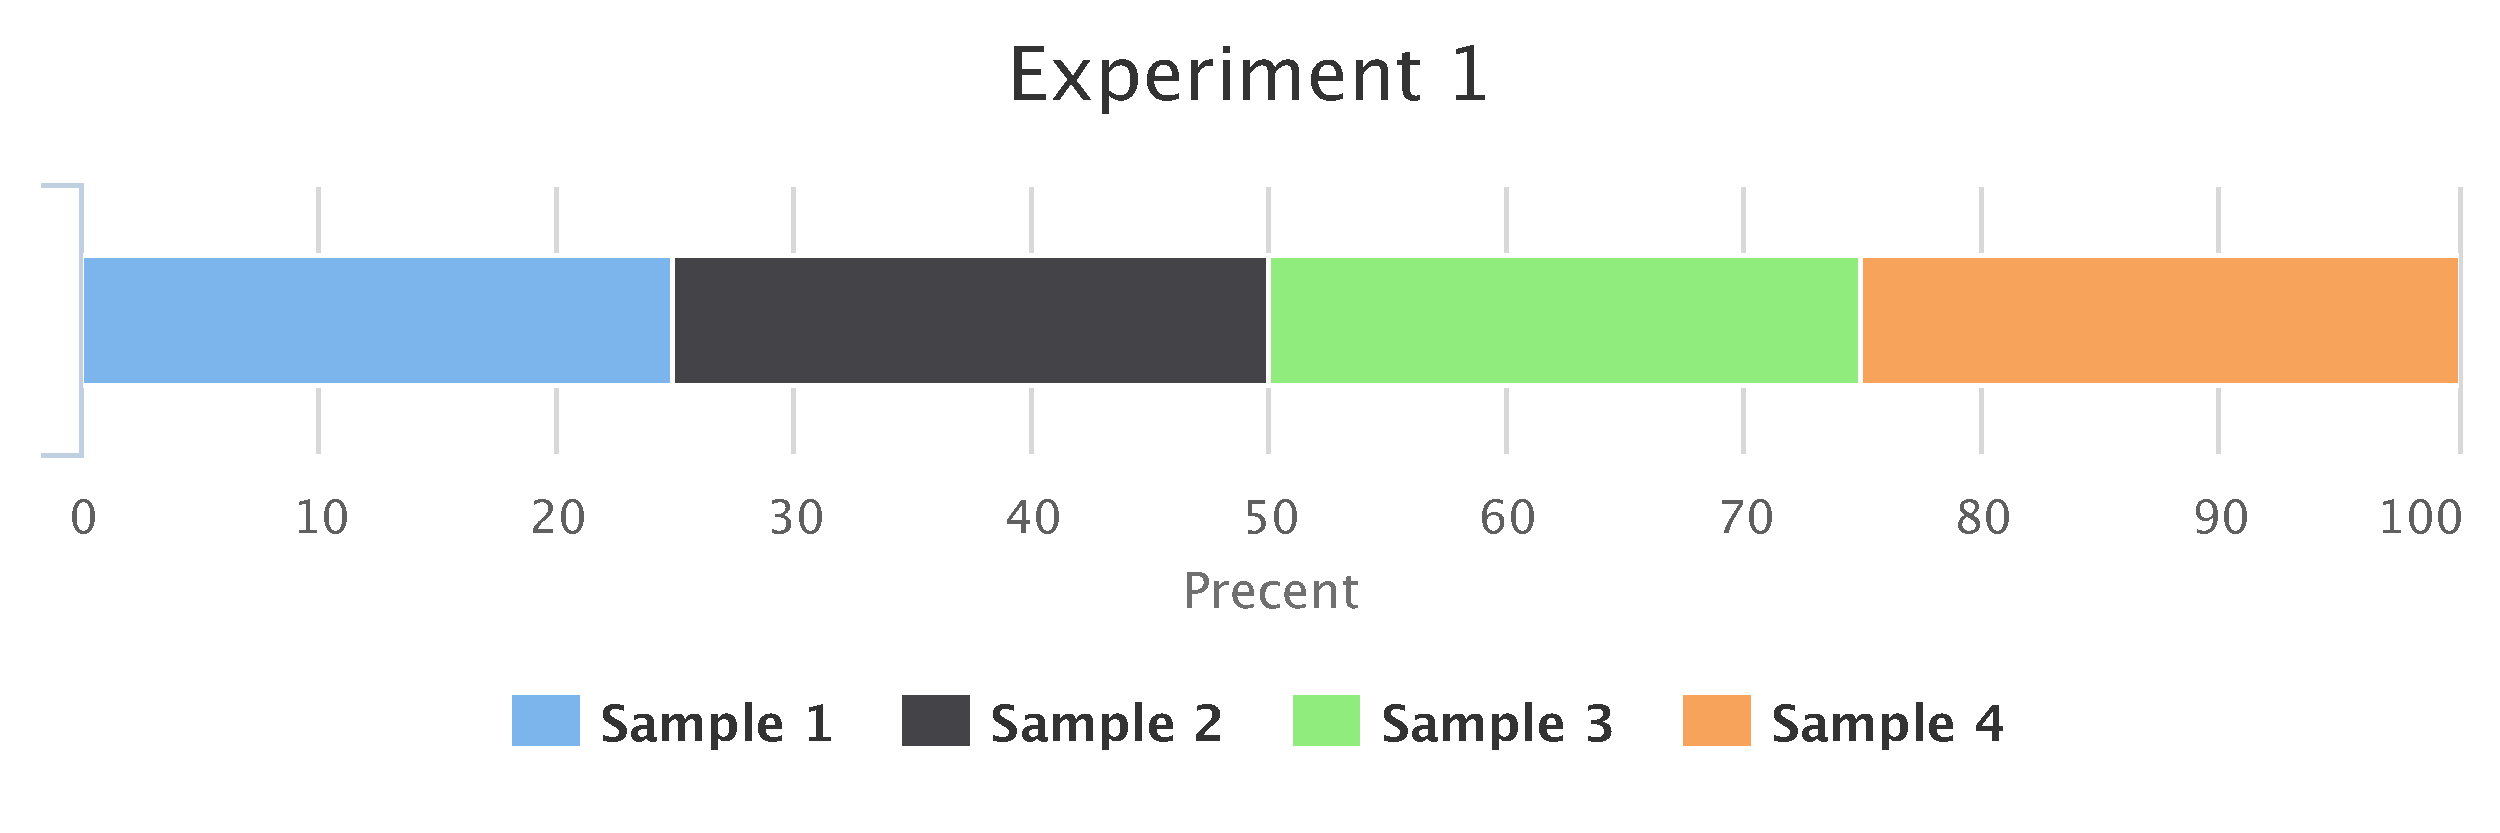
\includegraphics[width=1.0\textwidth]{images/exp_1_data}
%     \caption{Experiment 1 Data Sample Range}
%     \label{fig:exp_1_data_range}
% \end{figure}

%\subsection{Experiment 2}

% TODO show results
%To address the fixed data sampling used previously random sampling was employed. The number of samples $n$ was not changed from the first experiment. The prediction results improved slightly. The \gls{svm} model also reported an error relating to \textit{max number of iterations reached}. This error indicates that the \gls{svm} model is having trouble effectively separating the two categorizations of data into two distinct sets. Such warnings could mean that the features used for training the model are not linearly separable.

% TODO show a picture of how the data was divided.

% \subsection{Experiment 3}

% % TODO talk about using easy.py
% Further investigation into \gls{svm} lead to a research tool that provided grid search for optimizing the parameters used for a \gls{svm}. The results of these experiments offered improvements over the previous, however required a long time to find the right parameters and works the best with the dataset $data_i$ that was used to find the parameters.

% \subsection{Experiment 4}

% % TODO get experiment results
% Modified the candidate features set to test the \gls{svm} with. Added ones like change frequency, average time between commits, number of commits since last change, time since last change and previous change type. Dropped commit author in favor of using just committer. Finally changed the prediction to predict the whether a change will occur within the next 5 commits. In terms of the methodology, 2 variations were tested. The first one was predicting changes to a methods within the same package. The second one was prediction changes to a method within the same file. Neither of these changes provided substantial improvements since they reduced the available sample size, $|data_i|$, down so that the no reasonable predictions could be made from the reduced set.

% \subsection{Experiment 5}

% The next set of experiments required more complex features which necessitated more complex queries from the database. In fact the database interface in use, MySQL, was unable to implement some of the queries. MySQL only allows 2 levels of nested queries and has a more restrictive data type set. An alternative database interface PostgreSQL was used as a replacement for MySQL. PostgreSQL offers fair more sophisticated data types as well as \gls{cte}. The migration from MySQL to PostgreSQL was simplified through the use of pgloader as mentioned in \autoref{sec:storage}. 

% Another change was the even out the number of samples collected from each category. The data set $data_i$ tended to provide unbalanced categorization of the data. The same number of samples from each $n/2$ was collected to prevent biasing in the data set. A \gls{svm} model like most other machine learning algorithms is susceptible to category biasing. This will occur when the training set consists of $80\%$ of one category and $20\%$ of another. The model will train such that it always predicts the first category. This works out well if the data is always unbalanced in the same way however it will fail to predict the smaller category entirely. Therefore providing an even sample of each category ($50\%$ each) will prevent poor prediction results.

% Another result of determining that the data set was unbalanced in terms of the categorization was to calculate both precision and recall of the results. Accuracy alone only provides a very simple measure of how well the model predicted the samples from $data_{i+1}$. A clearer understanding is available with these three measures. Also with each provided an attempt can be made to optimize all three.

% Finally the last few tests in this experiment set included a new feature. This feature was the difference in time between the previous commit with a change and the latest commit. This feature was not particularly useful however and caused the data to become inseparable.

% At the end of this set of tests it was apparent that a deeper understanding of the candidate features was necessary to improve the results. Therefore an analysis of each candidate feature was performed both on the quality of the feature and the possible relationship with others. \gls{svm} models are particularly sensitive towards dependencies between the variables. It was also necessary to properly convert data into a format that could be used by the database. This was talked about in more detail in \autoref{subsec:svm_prediction}.

% \begin{table}
% \begin{center}
%     \begin{tabular}{|l|l|l|}
%         \hline
%         Project & Sample Size (n) & Accuracy \\
%         \hline  
%         acra & 100 & $70\%$ \\
%         acra & 1000 & $52\%$ \\
%         \hline
%     \end{tabular}
% \end{center}
%     \caption{Experiment 5 Results}
%     \label{tab:experiment_5_results}
% \end{table}

% \subsection{Experiment 6}

% After analyzing the candidate features a more ideal set of features was created. The tests were preformed again using sample sizes of $100$ and $1000$. After the changes were made to the data, the performance improved however some of the features did not prove as useful. However the improvement was marginal and therefore necessitated shift in focus from the features to the prediction method. Specificity the data sampling method was inspected to attempt improve the prediction results. Instead of breaking the data set into four even sets based on the date range the data was divided into two even sets based on date as shown in \autoref{fig:exp_6_data_range}

% \begin{figure}[!ht]
%     \centering
%         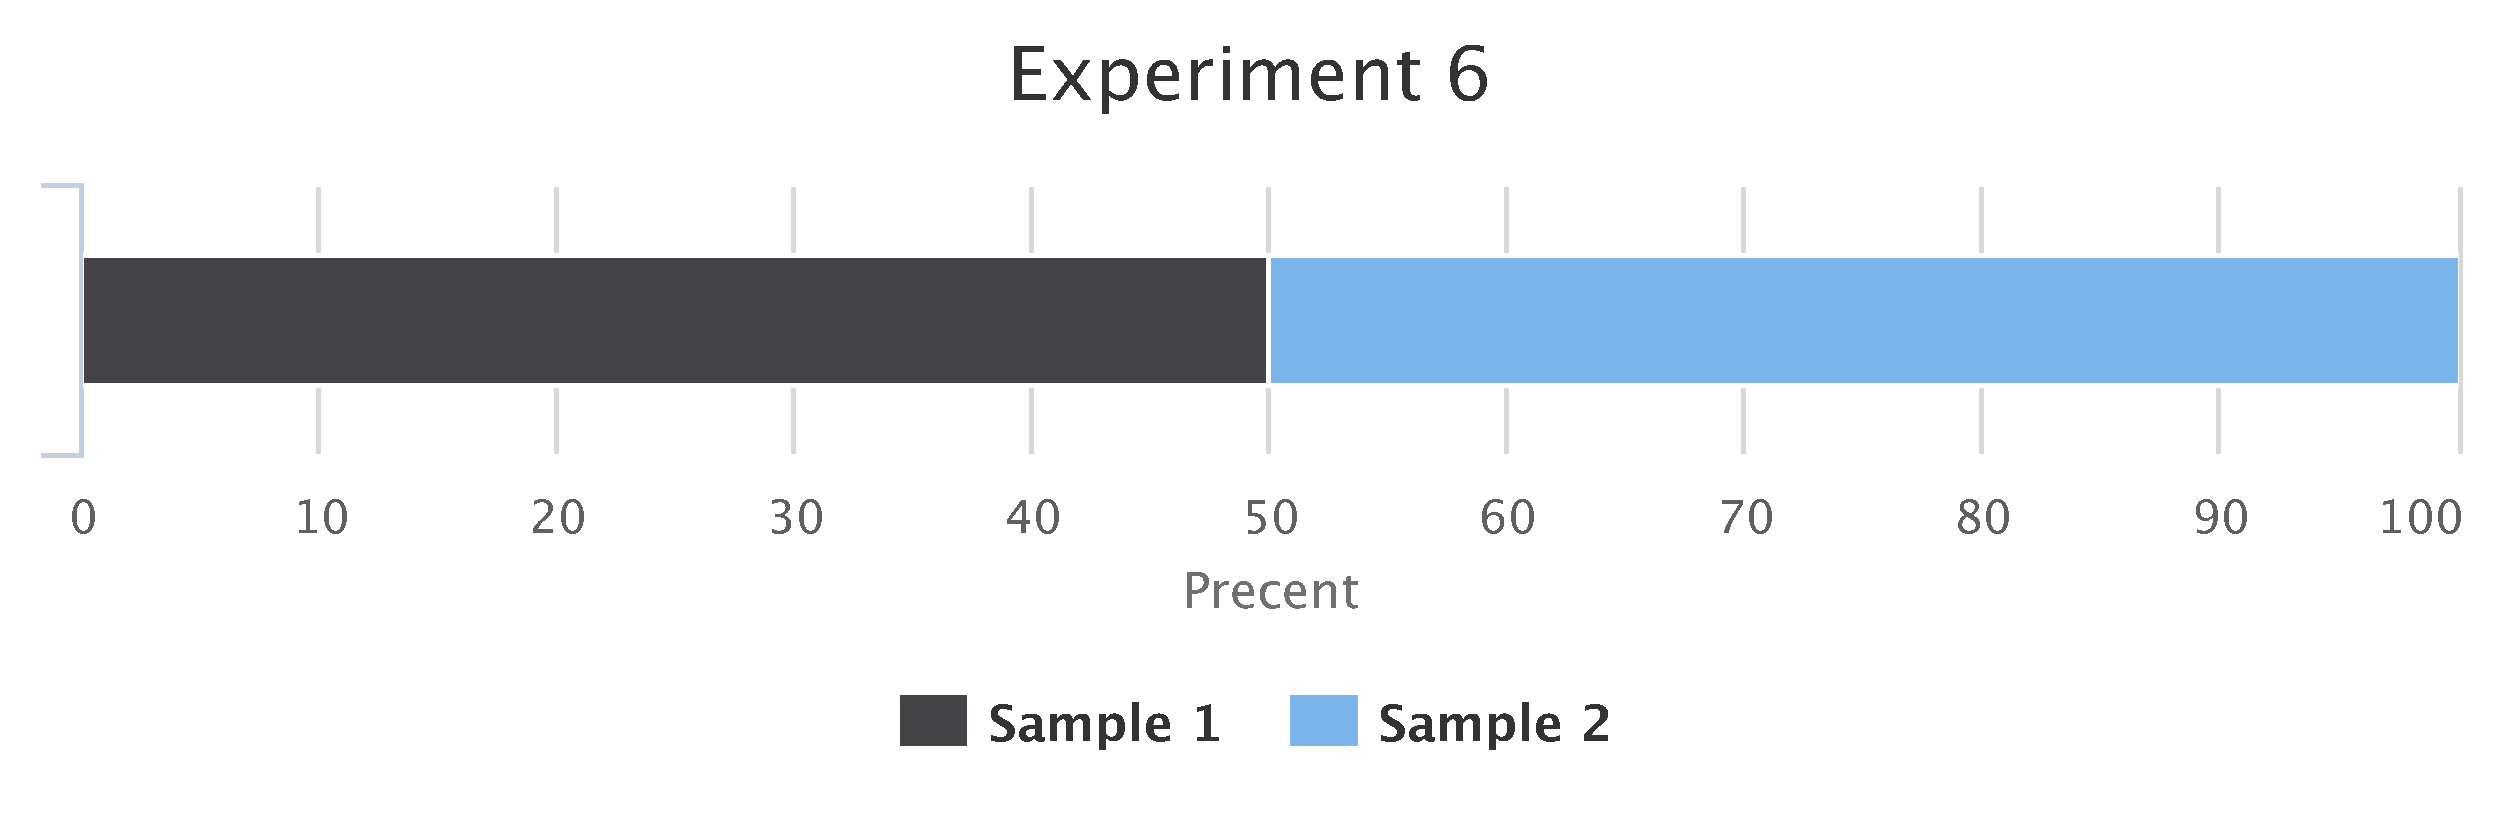
\includegraphics[width=1.0\textwidth]{images/exp_6_data_range}
%     \caption{Experiment 6 Data Sample Range}
%     \label{fig:exp_6_data_range}
% \end{figure}

%The results of the experiment are outlined in \autoref{tab:experiment_6_results}. The larger sample with $n = 1000$ is far worse than with $n = 100$. This however was a worse result than when the data set was divided into 4 equal parts.

% \begin{table}
% \begin{center}
%     \begin{tabular}{|l|l|l|}
%         \hline
%         Project & Sample Size (n) & Accuracy \\
%         \hline
%         acra & 100 & $60\%$ \\
%         acra & 1000 & $47\%$ \\
%         \hline
%     \end{tabular}
% \end{center}
%     \caption{Experiment 6 Results}
%     \label{tab:experiment_6_results}
% \end{table}

% \subsection{Experiment 7}

% Reorganized the data sampling method to sample based on commit ranges rather than date ranges. Instead of splitting the data set into four even sections, the sample range is taken from the current commit $c_i$ to $c_{i-m}$ in the case that $i > m$. $m$ denotes the width in commits of the sample space. For example if the model is predict a change that occurs within the next 5 commits and $m = 30$ then \autoref{fig:data_range} shows how the data would be sampled. The training sample would be where data would be collected from to train the model. The prediction gap is to account for the data sampling calculating whether methods at commit 40 will have a change within the next 5 commits. Therefore to properly test it on data that is not used as part of the testing model the offset is needed. The testing sampling section is the same size as the training sampling data set and follows the 5 commit gap.

% \begin{figure}[!ht]
%     \centering
%         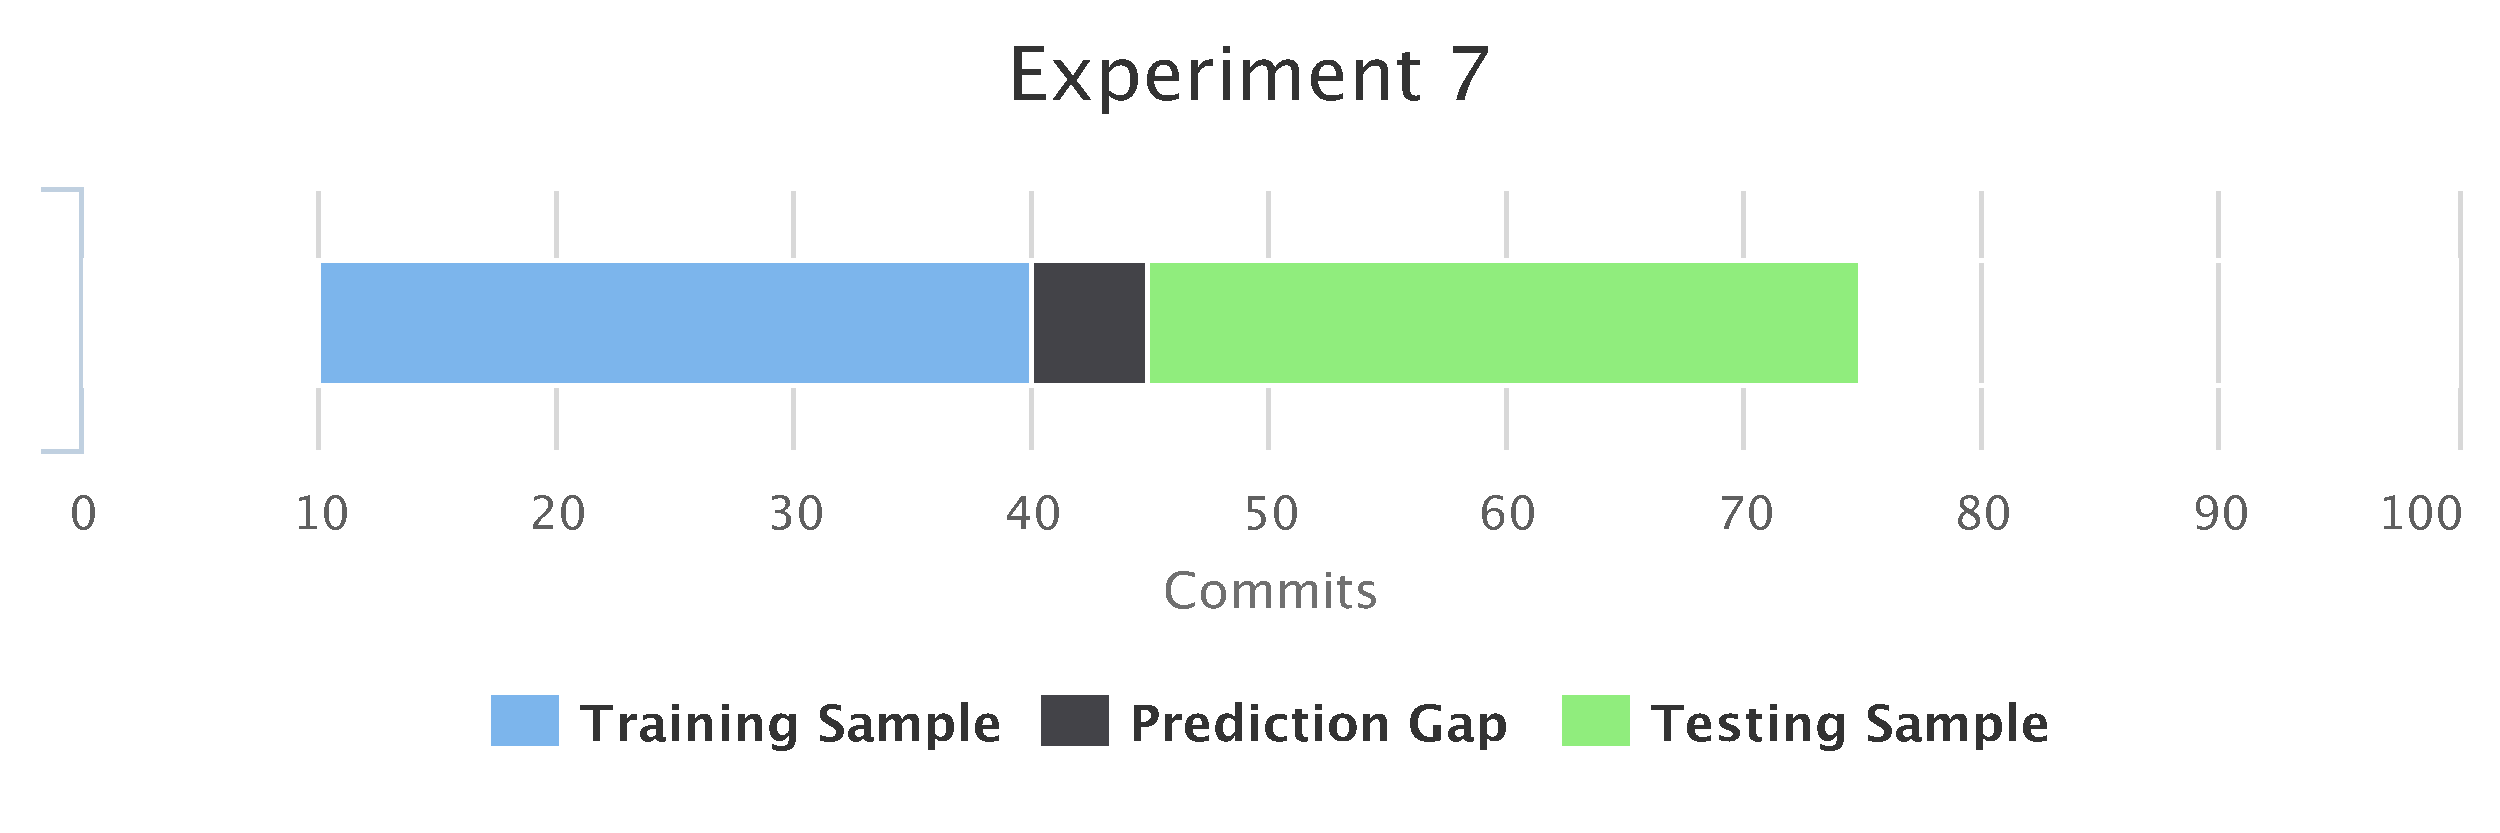
\includegraphics[width=1.0\textwidth]{images/exp_7_data_range}
%     \caption{Experiment 7 Data Sample Range}
%     \label{fig:data_range}
% \end{figure}

% Another change to the sampling method was to sample a percentage of the data within the sample rather than a fixed amount. The sample ranges provided a larger range of data to sample and thus sticking to a arbitrary amount of tuples was updated. This however introduced biasing issues with the data set since typically one category or the other had the majority of tuples within the sample. Fixing this issue is talked about in further detail in \autoref{subsec:random_forest_predictions}. Similar to the previous sampling techniques the data set was sampled randomly. Therefore the percentage of data sampled had a large impact on how long it took to train the model but typically also on the prediction results of the model. 

% TODO discuss the results

% \subsection{Experiment 8}

% After more or less establishing a data sampling model the candidate feature set was looked at again in an attempt to improve the prediction results. A few of the candidate features were removed and a minimum candidate feature set was determined which provided the best results for the current test project \textit{acra}.

% % TODO show some results

% % TODO outline the candidate feature set that performed the best for SVM

% The optimal value of $m$ is a more challenging issue since for project which have a large amount of rapid change occurring in the project larger value seems to provide a more positive result. Where as smaller projects or ones that have a slower rate of change tend to do far better with a smaller value of $m$. 

% \subsection{Experiment 9}

% After the results of the previous experiments proved to less consistent for other data sets such as \textit{storm} and \textit{fresco} another prediction algorithm was tested. \gls{rf} as discussed in greater detail in \autoref{subsec:random_forest_predictions} is more capable with unbalanced datasets and is generally more widely used for performing predictions on mined data. % TODO cite this.

% \gls{rf} while proving to be at times easier to get better results also had some of the challenges that the \gls{svm} model experienced. For example the best features to use in the prediction model and also the best commit width ($m$) to optimize the results.

\section{Experimental Setup}

\subsection{Prediction Features}

%The experimental process for testing the various feature sets on acra involved dividing the repository into four equal quarters (based on time duration). While the number of commits within each period may vary greatly, only a sample is taken.

    %- Alternatively the periods could be distributed such to make the number of commits equal between the sections. Further testing is needed to determine which method is more ideal.

%The \gls{svm} model was trained to categorize whether the current method would be changed within the next 5 commits. This of course can generalize to whether a vector will have a commit within the next \textit{n} commits. Obviously each candidate feature leverages historical or current information and thus a vector can be generated without future information.

%238, ReportField.java            |           8234 | public boolean getValue() {                                                                          |           0 | william-ferguson-au |  0.0464135021097046 | ("{3,3,0,0,0}","{68,1816,549469,779372,208198}")                              |        0
% TODO update this list based on new candidates
\begin{table}
\begin{center}
    \begin{tabularx}{\linewidth}{|l|X|l|l|}
        \hline
        Feature & Description & Data & Example Vector \\
        \hline
        $name$ & The name of the file & Main.java & 3 \\ \hline
        $signature$ & The method name related to the change details & void work() \{ & 46\\ \hline
        $change_i$ & Whether the method changed or not at the current commit & 3 & 1 \\ \hline
        $committer$ & The individual who committed the change & bob & 5 \\ \hline
        $freq_{change}$ & The number of changes this method has been involved divided by the number of commits up till this point & 0.0464 & 0.0464 \\ \hline
        $change_{prev}$ & A list of whether the method changed or not for the last 5 commits & \{3,3,0,3,1\} & \{1,1,0,1,1\} \\ \hline
        $\Delta t$ & A set of time deltas between the last 5 commits that involved the method & \{68,416,569,772,898\} & \{68,416,569,772,898\} \\
        \hline
        $change_{next\_6}$ & Identifies whether at least one change occurred within the next 5 commits for the given method & 0 & 0\\
        \hline
    \end{tabularx}
\end{center}
    \caption{Candidate features for \gls{svm} model}
    \label{tab:candidate_features}
\end{table}
%& \{68,1816,5469,7772,8198\} 

% Name => Methods within a file are likely going to have similar change patterns
% Signature => A method change history will likely be unique
% Change_i => Whether the method changed or not at the current commit may provide insight as to whether the next 5 commits will feature a change as well.
% committer => Users may change in different change patterns thus helping identify whether this will be a change or not, 
% freq_change => Helps identify how likely the file is to change

The \autoref{tab:candidate_features} lists each feature with a more detailed description. An example of each feature is provided to further illustrate them. As stated in the previous \autoref{subsec:svm_prediction}, the values need to be first converted into floating point numbers. First the data is extracted from the database as \textit{raw} values as shown in the \textit{\textbf{Data}} column. Taking the $name$ value, ``Main.java'' will be mapped to the value 3. This is because 2 other methods have already been mapped and therefore method name is mapped to the next available mapping, 3. Similarly both $signature$ and $committer$ will be mapped from their respective values ``void work() \{'' and ``bob'' to 46 and 5. Numerical values are easily converted by casting them to floating point values if they are not already of that type. For spacing reasons all the values in the table that were integers to begin are shown without a ``.0''following.

Another small change made to the data to create a vector for the \gls{svm} model was to apply \autoref{eq:change_type} to the values of $change_i$ and $change_{prev}$. As in \autoref{tab:candidate_features}, the value of $change_i$ is initially 3 which indicates a modification occurred. Since a modification is a type of change $C(change_i) = 1$ which is the value used by the vector. Likewise this is also applied to each entry in the $change_{prev}$ changing it into a bit vector.

\begin{equation} 
\label{eq:change_type}
C = \left\{\begin{matrix}
1 & \text{if} change > 0 \\
0 & \text{otherwise}
\end{matrix}\right.
\end{equation}

Both $change_{prev}$ and $\Delta t$ are actually each 5 features since they are a set of features. $change_{prev}$ shows the type of change that occurred for the last 5 commits. Similarly $\Delta t$ shows the difference between the current commit time ($t(c_i)$) and the previous commit time ($t(c_{i-1})$) calculated in \autoref{eq:time_delta}. These two features then expanded to add a new category for each entry in the set. The ordering is maintained since each entry maps to a previous commit in order.

\begin{equation}
\label{eq:time_delta}
\Delta t_{i} = t(c_i) - t(c_{i-1}), i > 1
\end{equation}

% TODO place in a better spot.
$freq_{change}$ is calculated as by taking the number commits which involve changes to the current method ($c_i$) divided by the current number of commits ($c_{cur}$).
\begin{equation}
\label{eq:freq_change}
freq_{change} = \frac{|c_i|}{|c_{cur}|}
\end{equation}

% TODO provide how to calculate the other features.

%TODO write algorithm for mapping names

% TODO put this into the subsection experiment 8-9
Another issue that was necessary to address was the arbitrary sample size. For projects that are a lot bigger 100 vectors which map to 100 method changes could be very small. The sampling also seemed like a peculiar approach to picking the data since it would randomly pick values from over a period that could vary from a few months to a few years depending on the size. Therefore instead of dividing the project into four quarters based on time a number of commits is picked. The test is then designed around a given date with the \textit{gap} with $t$ and $p$ commits proceeding it as the range of the test. $t$ is the number of commits that the training dataset will sample from. Alternatively, $p$ is the number of commits that the testing dataset will sample from. In the case that $t = p$ the training commit size and the testing commit size are the same.

The final change that was accounted for was to change the population sample size from a fixed number to a percentage. This allows more flexibility and determining the sample size of a test by allowing for it to scale based on the size of the project. 

% TODO show a final picture with population size as a percentage.

% TODO access this stuff below. Remember It's now 5 commits not 6 and also a lot of this stuff is no longer relevant.

The initial thought was to provide a few different features that appeared to be unique and potentially provided useful information for whether the method will change within the next 5 commits. Of course since this measurement is calculated, if a vector within the sample set is within the last 5 commits then it will leverage data from the next quarter to provide its prediction. This has not been mitigated and could provide a unrealistic improvement in the prediction score if members of the next sample fall into the first 5 commits. The way to mitigate this would be to provide a buffer between the two sets when the second test is used for testing purposes. The second set would be restricted further, such that the changes must come from after the 6th commit from the start date of the quarter. The first commit would be the one that takes place on or right after (if no commit falls on that date) the start date. The next 5 commits would also be excluded from the test sample set.

\subsection{Experiment Factors}
% TODO outline the different factors used in the experiments. Also even outline other factors that are not changed either.

% Factors:
% Sliding Window
% Extended sampling ranges
% Training Range
% Testing Range
% Sample Range by Commit (or by date)
% Oversampling
% Undersampling
% Dynamic Size of sampling
% Sampling Percent
% Sampling Randomly
% Window
% SVM or Forest Parameters

Reorganized the data sampling method to sample based on commit ranges rather than date ranges. Instead of splitting the data set into four even sections, the sample range is taken from the current commit $c_i$ to $c_{i-m}$ in the case that $i > m$. $m$ denotes the width in commits of the sample space. For example if the model is predict a change that occurs within the next 5 commits and $m = 30$ then \autoref{fig:data_range} shows how the data would be sampled. The training sample would be where data would be collected from to train the model. The prediction gap is to account for the data sampling calculating whether methods at commit 40 will have a change within the next 5 commits. Therefore to properly test it on data that is not used as part of the testing model the offset is needed. The testing sampling section is the same size as the training sampling data set and follows the 5 commit gap.

\begin{figure}[!ht]
    \centering
        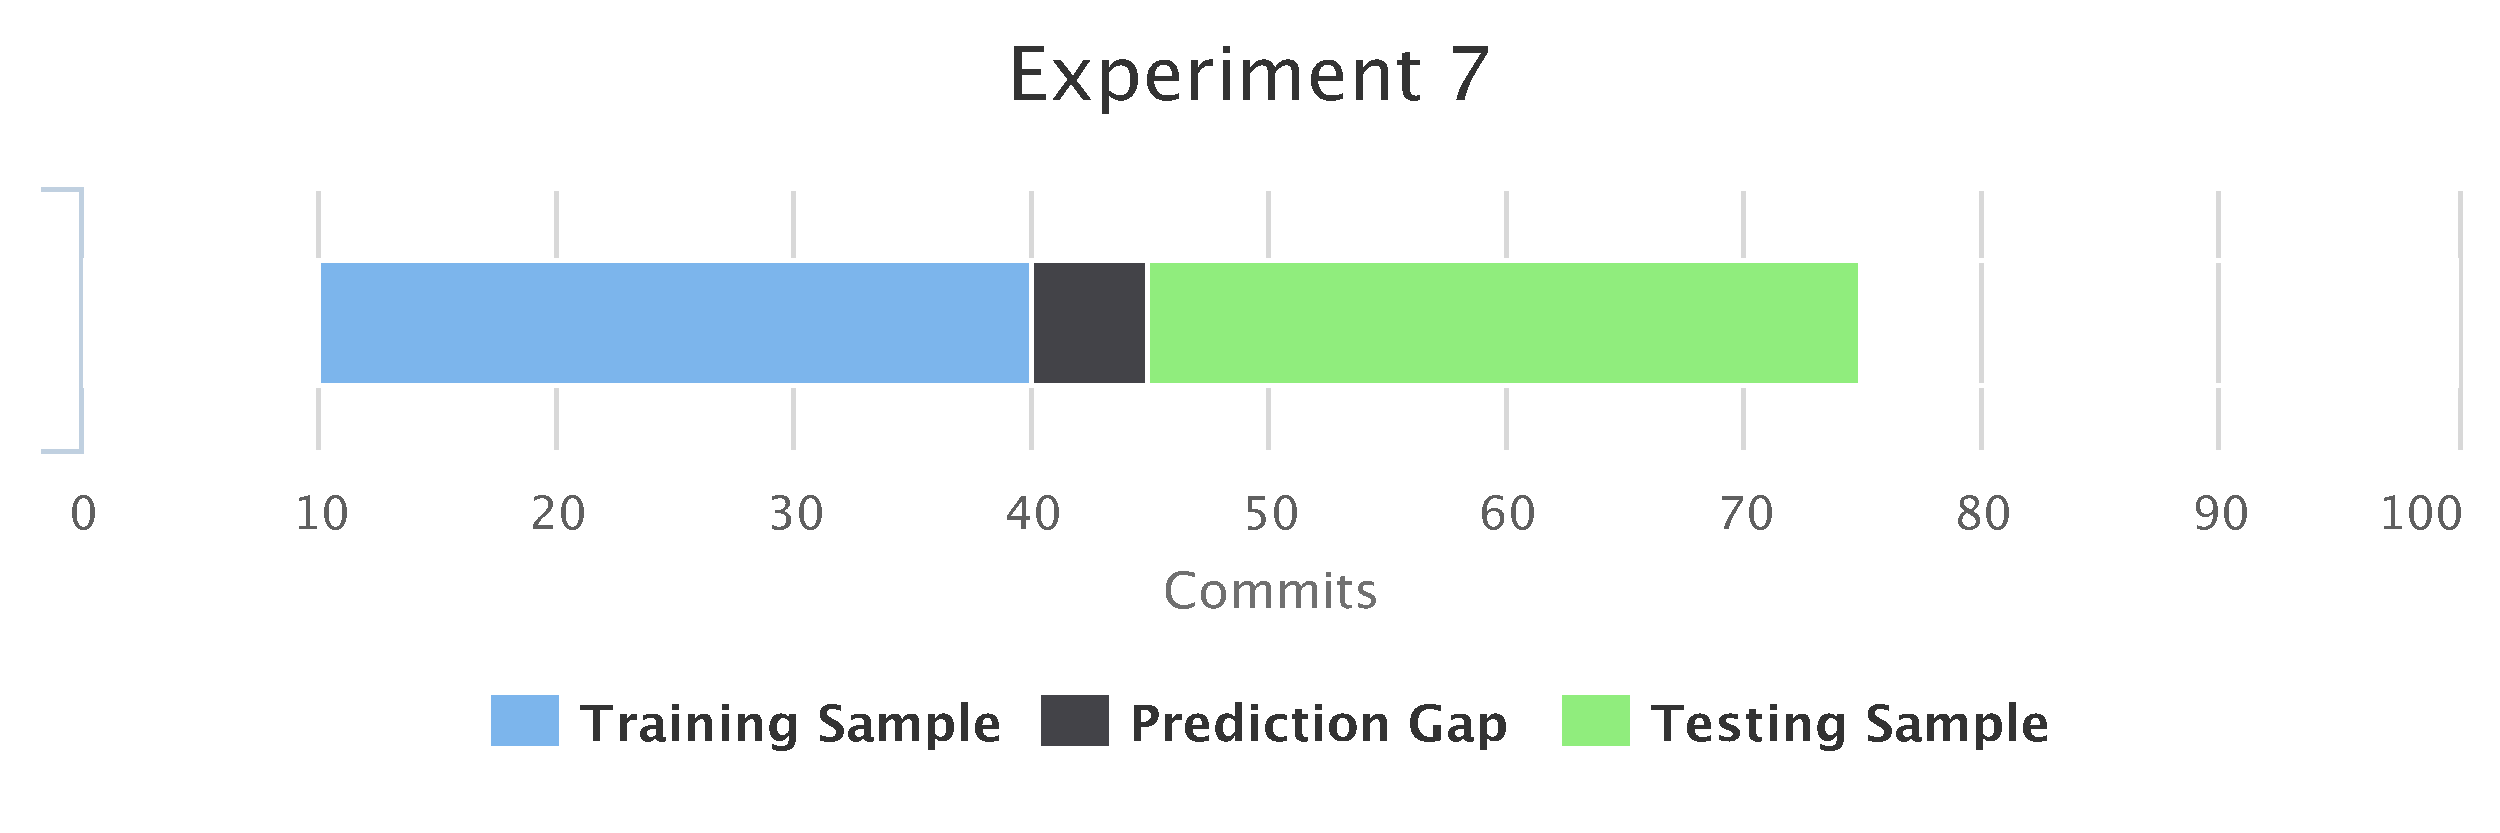
\includegraphics[width=1.0\textwidth]{images/exp_7_data_range}
    \caption{Experiment 7 Data Sample Range}
    \label{fig:data_range}
\end{figure}

The sliding window factor is one of core aspects related to extracting samples from the data set. When using the sliding window to sample the data the data is divided as shown in \autoref{fig:data_range}. The training sample is where the training data set is sampled from. The testing sample is where the testing data is sampled from. 

A data set with an extended sampling range will extend the sampling range beyond the original size for either the training sample or the testing sample. The training range can be expanded to include earlier samples to increase the sample space.

The training and testing sampling range are defined as the number of commits from which the samples can be taken. In \autoref{fig:data_range}, both the training and testing sample ranges are set to 30 commits. These two values can differ from one another but tend to be kept the same for most of the experiments.

Two other factors in the experiments was handling the data set bias. The two methods are oversampling and undersampling of data elements. Most of the time a data set will contain more samples in one category than the other. When the number of samples in each category is very close this will have little effect on the model. However in cases were the data is highly skewed to one classification over the other the model will simply predict the larger classification. Use of oversampling will take more samples (duplicates) from the smaller classification to be closer in size to the larger classification. Alternatively, undersampling will use remove samples from the larger classification to become closer in size to the smaller classification.
% Discussed further in section in approach

Another feature assessed was that of the sample size. The sample size was determined by the sample ratio. When sampling if the ratio is at 50 \% then only half of the values retrieved will be used to train or test. For some of the larger data sets sampling 100 \% of the data from the range would take a lot longer. Therefore sampling a percentage of the data set is commonly used to decrease the training time. However in the case of using a percentage of the sample range the data should to be sampled randomly to provide a more stable model. Therefore each data entry in the sample has the same chance to be within the training or test data set.

For each project data set there are numerous windows that be can be used. The window number is setting which window is used broadly mapping to the position within the data set that the model will be trained on and then predicted on. As shown in \autoref{fig:data_range}, the window is shown starting at the 30th commit which would also be called the 30th window.

Finally, the last factor of note is the parameters used to configure each prediction method. \gls{rf} use a single parameter, the size of the forest. \gls{svm} meanwhile uses three parameters; C, gamma and esp. % TODO explain each of them in a bit more details.

\subsection{Prediction Performance}

% TODO this isn't necessary for cases when the entire sample is used.
For each experiment where the used random sampling the experiment was performed 5 times to account for variations in the random sample. Therefore if the initial results using the first sample set were not characteristic of the full dataset then running the experiment with more random samples is more likely to represent the true characteristics of the dataset. This required taking five random samples from each quarter, training the model and running the tests on the model to then determine the average prediction score. In the case when $100\%$ of the sample is used then only one sample is is taken since there will be no variations within the sample set.

The goal of the prediction methods are to provide a good prediction of whether the a given vector will fit in one category or the other. A model's prediction performance can be rated using three measures of accuracy, precision and recall. Accuracy is measured as how often predictions $p$ are classified correctly where $a_i$ represents vector $v_i$ correct classification. The algorithm for calculating a single vectors accuracy is showing in \autoref{eq:vector_accuracy}. The prediction accuracy ($P_{accuracy}$) can then be calculated using \autoref{eq:prediction_accuracy}. This simply sums up the accuracy for each vector and then divides it by the total number of vectors (where $n = |v|$).

\begin{equation} 
\label{eq:vector_accuracy}
v_i = \left\{\begin{matrix}
1 & \text{if } p_i = a_i\\ 
0 & \text{otherwise}
\end{matrix}\right.
\end{equation}

\begin{equation}
\label{eq:prediction_accuracy}
P_{accuracy} = \frac{\sum_{i=0}^{n}v_i}{n} \times 100
\end{equation}

The precision of a model is the measure of how correct the model predicts that a change will occur when it predicts that a change will occur. Given the true positives $tp$, represents the number of predictions that the model correctly identified as having a change and the false positives $fp$ is the number of times the model incorrect predicted a change to occur when it in fact did not. The equation for calculating precision is show in \autoref{eq:precision}.

\begin{equation} 
\label{eq:precision}
P_{precision} = \frac{tp}{tp+fp}
\end{equation}

The recall of the model is the measure of how correct the model predicts that change will occur out of all the times changes really occurred. Again using $tp$ as the number of true positives, and false negatives $fn$ which is the number of times the model fails to predict that a change will occur. The recall can be calculated using the \autoref{eq:recall}

\begin{equation} 
\label{eq:recall}
P_{recall} = \frac{tp}{tp+fn}
\end{equation}

\section{\gls{svm} Experiments}
\label{sec:svm_experiments}

The experiment is setup to have a set of parameters that can be set. These parameters will remain constant to observer the difference that the independent variable will have on the dependent variables, precision, recall and accuracy. Each experiments will use one of the parameters as the independent variable. 

\subsection{Window Range Experiments}

%TODO fill out details of experiments

For this experiment the variable was the size of the sample window range in commits. In \autoref{tab:window_range_experiment_features}, the features used by the prediction model are outlined. Features with a mark, $\bullet$, are used while those without are not. In this experiment only the Short $\Delta_{freq}$ is not used while all the rest are.

% TODO use a better way of showing this like a table with dots.
\begin{table}[h]
\begin{center}

    \begin{tabular}{|c|c|c|c|c|c|c|c|}
        \hline
        Com & Sig & Name & $\Delta_{freq}$ & Short & $t_{i} - t_{i-1}$ & Length & Has \\
         & & & & $\Delta_{freq}$ & & & Next \\ \hline
        $\bullet$ & $\bullet$ & $\bullet$ & $\bullet$ & & $\bullet$ & $\bullet$ & $\bullet$ \\ \hline
    \end{tabular}
    \caption{Window Range Experiment Features}
    \label{tab:window_range_experiment_features}
\end{center}

\end{table}

%% TODO create a table to show this information.
% Extend Window: No% Sample by Commit Range: Yes
% Over Sampling: No
% Under Sampling: Yes
% Sample Rate: 100%
% Window Offset: 5
% SVM c: 10
% SVM gamma: 8
% SVM esp: 0.001

As noted above the independent variable for this experiment is the sample window range. The remaining parameters for the experiment are constant for each test. The parameters for this experiment are outlined in \autoref{tab:window_range_experiment_setup}.

\begin{table}[h]
\begin{center}

    \begin{tabular}{|c|c|c|c|c|cc|}
        \hline
        Extended & Over & Under & Sample & Window & SVM & \\
        Window & Sampling & Sampling & Rate & Offset & C & gamma \\ \hline
        No & No & Yes & $100\%$ & 5 & 10 & 8 \\ \hline
    \end{tabular}
    \caption{Window Range Experiment Setup}
    \label{tab:window_range_experiment_setup}
\end{center}

\end{table}

The results for the experiments are shown with the precision, recall and accuracy. For each graph the independent variable is the number of commits in the sample window range. Y-axis is the value of each of the different plot, either precision, recall and accuracy. The first project, acra, in \autoref{fig:test_1_acra_rf} has the strongest performance out of all the projects. The best performance for acra is at sample window range at 80 commits width.

\begin{figure}[h]
    \centering

    \begin{minipage}[b]{0.45\linewidth}
        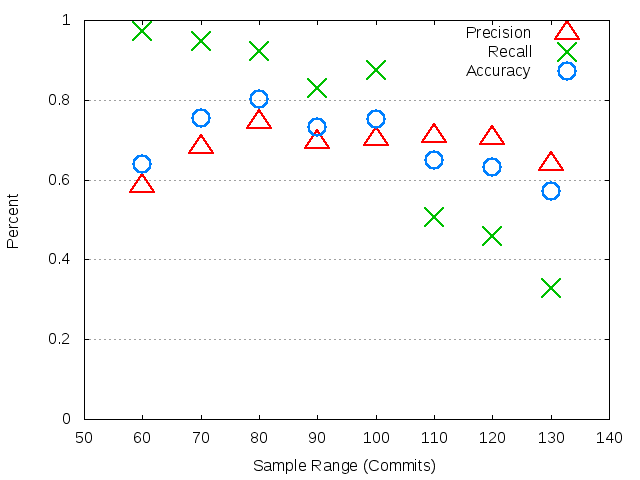
\includegraphics[width=1.0\textwidth]{images/svm/test_1/acra_sample_range}
        \caption{Sample Window Range for acra}
        \label{fig:test_1_acra_rf}
    \end{minipage}
\quad
    \begin{minipage}[b]{0.45\linewidth}
        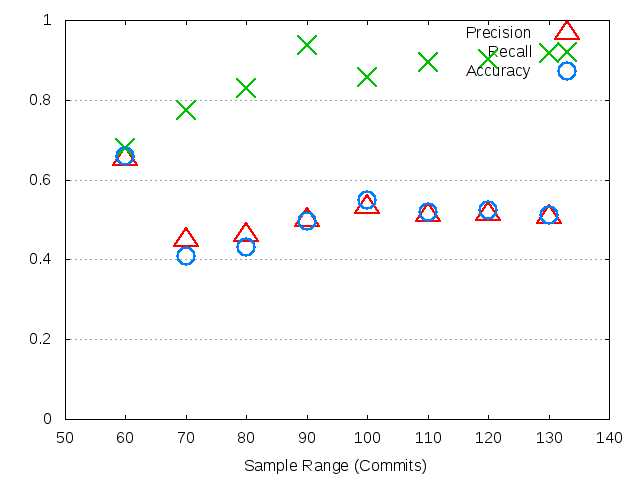
\includegraphics[width=1.0\textwidth]{images/svm/test_1/dagger_sample_range}
        \caption{Sample Window Range for dagger}
        \label{fig:test_1_dagger_rf}
    \end{minipage}
\end{figure}

\begin{figure}[h]
    \centering

    \begin{minipage}[b]{0.45\linewidth}
        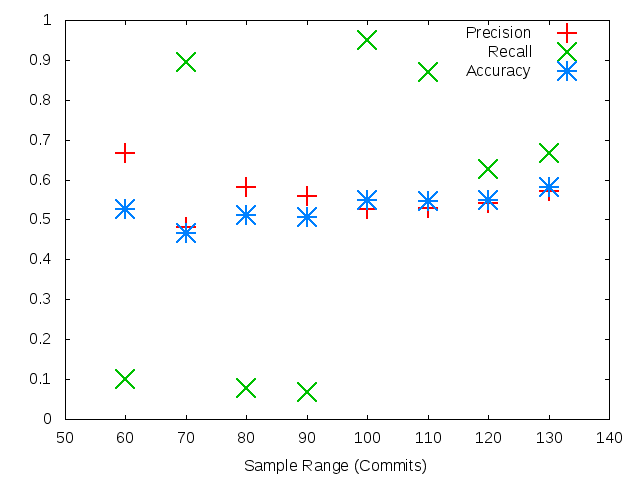
\includegraphics[width=1.0\textwidth]{images/svm/test_1/fresco_sample_range}
        \caption{Sample Window Range for fresco}
        \label{fig:test_1_fresco_rf}
    \end{minipage}
\quad
    \begin{minipage}[b]{0.45\linewidth}
        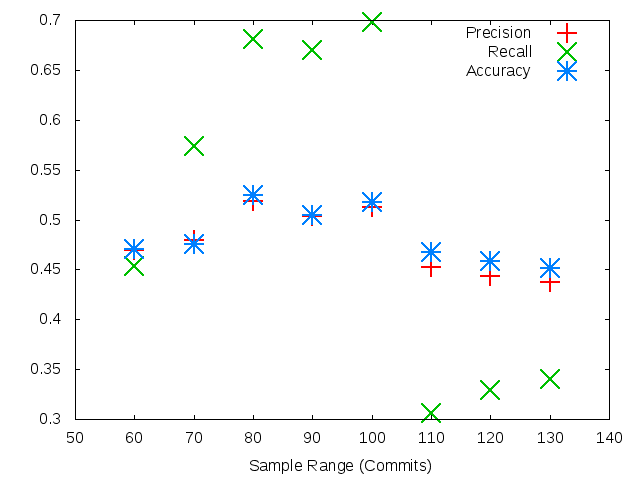
\includegraphics[width=1.0\textwidth]{images/svm/test_1/storm_sample_range}
        \caption{Sample Window Range for storm}
        \label{fig:test_1_storm_rf}
    \end{minipage}
\end{figure}

\begin{figure}[h]
    \centering
        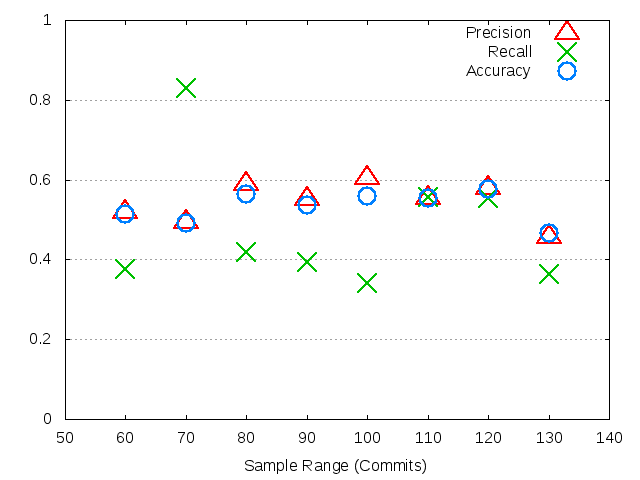
\includegraphics[width=0.45\textwidth]{images/svm/test_1/deeplearning4j_sample_range}
    \caption{Sample Window Range for deeplearning4j}
    \label{fig:test_1_deeplearning4j_rf}
\end{figure}

Alternatively, dagger has abysmal performance with the exception of a sample window range of 60. Fresco prediction performance does not particularly differ greatly. Also, it should be noted that the experiments with a sample window range of 120 and 130 since both resulted in a undefined precision and recall of 0 and accuracy of $0.5$.

Apache had slight variations, however the precision and accuracy never exceeded $0.55$. Finally, deeplearning4j does not have very good performance with low recall results. As shown in the plots, the sample window range has a significant impact on the performance of the model. While the actual width varies widely per project, there are projects with a width that fares worse and others that fare far better.

Overall there was no clear value for the sample window range which held consistent positive results. Generally speaking, projects that were smaller; acra, dagger, fresco, appeared to get positive results with smaller windows. Alternatively, larger projects; storm and deeplearning4j both did fairly poorly with the test range from 60 to 130. The largest project, deeplearning4j also has a slight positive trend towards the end of the range. However, storm does have a negative trend towards the end of the range.

The precision and accuracy remain fairly stable throughout this experiment. While the value of these attributes changes with different values of the sample window range these changes tend to be fairly close and follow a general trend. However for dagger in \autoref{fig:test_1_dagger_rf} the performance of accuracy and precision drops from $0.6 - 0.7$ range to $0.4 - 0.45$ range. The accuracy and precision also do however remain rather stable for the remainder of the experiments in this set.

Finally, the recall for the prediction is very unstable. While both accuracy and precision are very closely related and so will be likely close in value. Recall however will vary from a very low value to a very high value. For example in \autoref{fig:test_1_fresco_rf} the value of recall at sample window range of $60$ is $0.1$ and then jumps to $0.9$ at sample window range of $70$. \autoref{fig:test_1_storm_rf} and \autoref{fig:test_1_deeplearning4j_rf} both also have large changes in the recall but none as drastic as shown in fresco. 

% \begin{figure}[!ht]
%     \centering
%         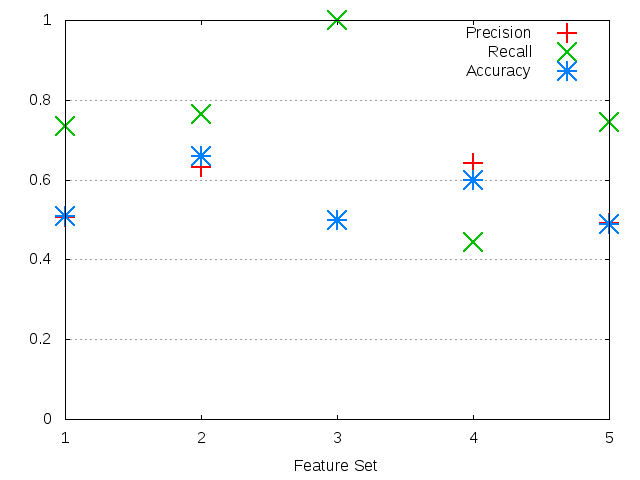
\includegraphics[width=1.0\textwidth]{images/test_1/dagger_sample_range}
%     \caption{Sample Window Range for dagger}
%     \label{fig:test_1_dagger}
% \end{figure}

% \begin{figure}[!ht]
%     \centering
%         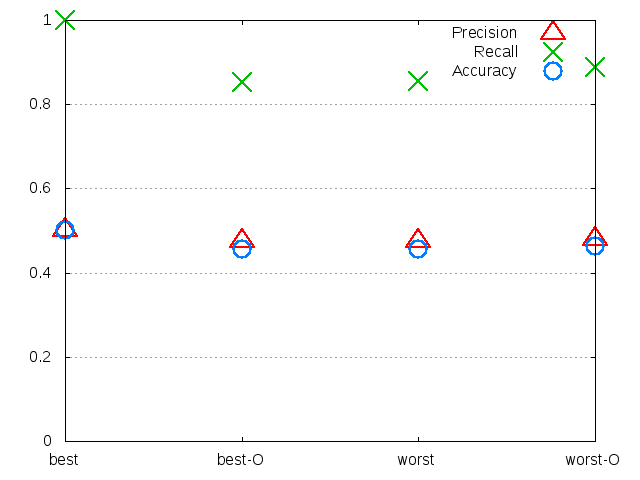
\includegraphics[width=1.0\textwidth]{images/test_1/fresco_sample_range}
%         \caption{Sample Window Range for fresco}
%         \label{fig:test_1_fresco}
% \end{figure}

% \begin{figure}[!ht]
%     \centering
%         \includegraphics[width=1.0\textwidth]{images/test_1/storm_sample_range}
%         \caption{Sample Window Range for storm}
%         \label{fig:test_1_storm}
% \end{figure}

% \subsection{Sample Window Range Experiments 2}

% For this experiment the variable was the size of the sample window range in commits. In \autoref{tab:window_range_experiment_features}, the features used by the prediction model are outlined. Features with a mark, $\bullet$, are used while those without are not. In this experiment only the Short $\Delta_{freq}$ is not used while all the rest are.

% \begin{table}[h]
% \begin{center}

%     \begin{tabular}{|c|c|c|c|c|c|c|c|}
%         \hline
%         Com & Sig & Name & $\Delta_{freq}$ & Short & $t_{i} - t_{i-1}$ & Length & Has \\
%          & & & & $\Delta_{freq}$ & & & Next \\ \hline
%         $\bullet$ & $\bullet$ & $\bullet$ & $\bullet$ & $\bullet$ & & $\bullet$ & $\bullet$ \\ \hline
%     \end{tabular}
%     \caption{Window Range Experiment Features}
%     \label{tab:window_range_experiment_features}
% \end{center}

% \end{table}

% %% TODO create a table to show this information.
% % Extend Window: No% Sample by Commit Range: Yes
% % Over Sampling: No
% % Under Sampling: Yes
% % Sample Rate: 100%
% % Window Offset: 5
% % SVM c: 10
% % SVM gamma: 8
% % SVM esp: 0.001

% As noted above the independent variable for this experiment is the sample window range. The remaining parameters for the experiment are constant for each test. The parameters for this experiment are outlined in \autoref{tab:window_range_experiment_setup}.

% \begin{table}[h]
% \begin{center}

%     \begin{tabular}{|c|c|c|c|c|cc|}
%         \hline
%         Extended & Over & Under & Sample & Window & SVM & \\
%         Window & Sampling & Sampling & Rate & Offset & C & gamma \\ \hline
%         No & No & Yes & $100\%$ & 5 & 10 & 8 \\ \hline
%     \end{tabular}
%     \caption{Window Range Experiment Setup}
%     \label{tab:window_range_experiment_setup}
% \end{center}

% \end{table}

% % TODO talk about results

% \begin{figure}[!ht]
%     \centering

%     \begin{minipage}[b]{0.45\linewidth}
%         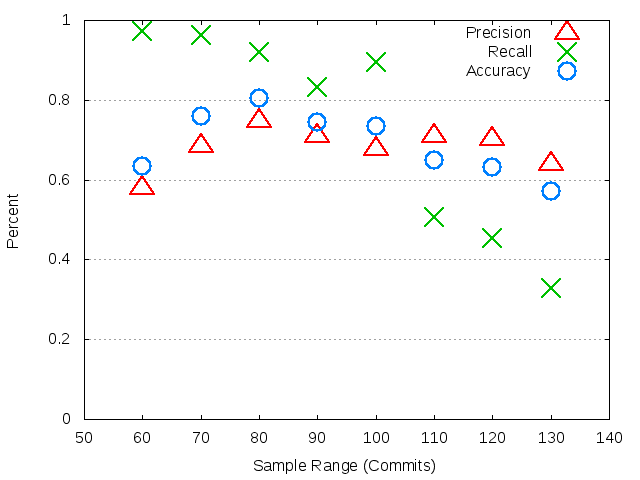
\includegraphics[width=1.0\textwidth]{images/svm/test_2/acra_sample_range}
%         \caption{Sample Window Range for acra}
%         \label{fig:test_2_acra}
%     \end{minipage}
% \quad
%     \begin{minipage}[b]{0.45\linewidth}
%         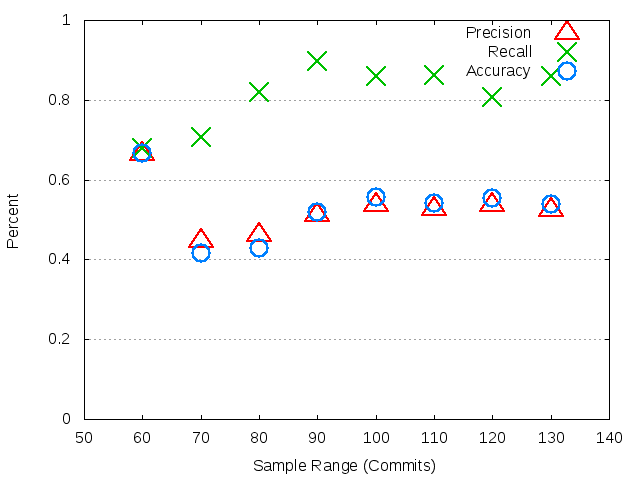
\includegraphics[width=1.0\textwidth]{images/svm/test_2/dagger_sample_range}
%         \caption{Sample Window Range for dagger}
%         \label{fig:test_2_dagger}
%     \end{minipage}
% \end{figure}

% \begin{figure}[!ht]
%     \centering

%     \begin{minipage}[b]{0.45\linewidth}
%         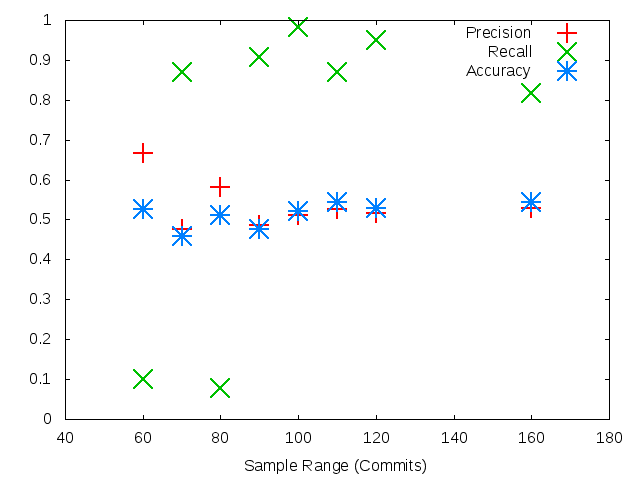
\includegraphics[width=1.0\textwidth]{images/svm/test_2/fresco_sample_range}
%         \caption{Sample Window Range for fresco}
%         \label{fig:test_2_fresco}
%     \end{minipage}
% \quad
%     \begin{minipage}[b]{0.45\linewidth}
%         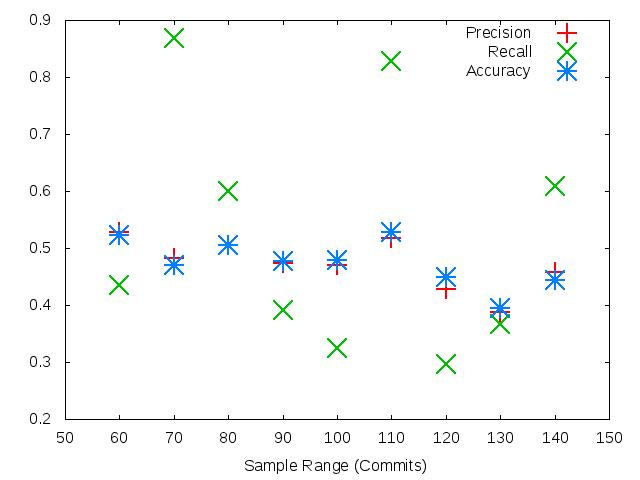
\includegraphics[width=1.0\textwidth]{images/svm/test_2/storm_sample_range}
%         \caption{Sample Window Range for storm}
%         \label{fig:test_2_storm}
%     \end{minipage}
% \end{figure}

% \begin{figure}[!ht]
%     \centering
%         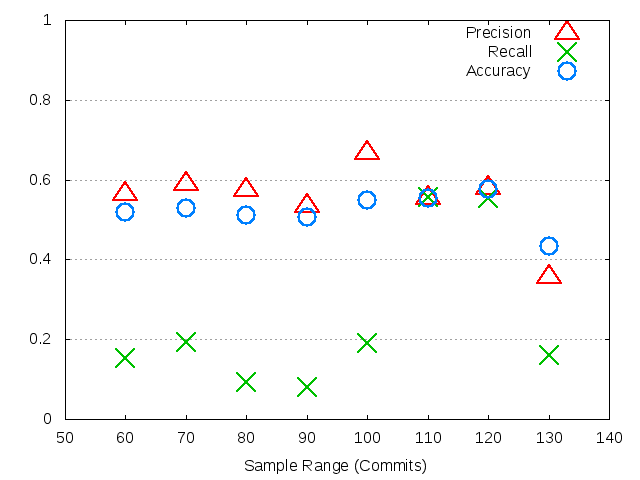
\includegraphics[width=0.45\textwidth]{images/svm/test_2/deeplearning4j_sample_range}
%     \caption{Sample Window Range for deeplearning4j}
%     \label{fig:test_2_deeplearning4j}
% \end{figure}



% TODO add a few more experiments.

\subsection{SVM Discussion}
\label{subsec:svm_discussion}

\section{Random Forest Experiments}
\label{sec:rf_experiments}

\subsection{Factor}

\subsection{Sample Window Experiments}

The independent variable for this set of experiments is the sample window size measured in commits. The candidate features are outlined in \autoref{tab:window_range_experiment_features}. Is the same as the first \gls{svm} experiment the candidate feature set.

\begin{table}[h]
\begin{center}

    \begin{tabular}{|c|c|c|c|c|c|c|c|}
        \hline
        Com & Sig & Name & $\Delta_{freq}$ & Short & $t_{i} - t_{i-1}$ & Length & Has \\
         & & & & $\Delta_{freq}$ & & & Next \\ \hline
        $\bullet$ & $\bullet$ & $\bullet$ & $\bullet$ & & $\bullet$ & $\bullet$ & $\bullet$ \\ \hline
    \end{tabular}
    \caption{Window Range Experiment Features}
    \label{tab:rf_window_range_experiment_features}
\end{center}

\end{table}

%% TODO create a table to show this information.
% Extend Window: No% Sample by Commit Range: Yes
% Over Sampling: No
% Under Sampling: Yes
% Sample Rate: 100%
% Window Offset: 5
% SVM c: 10
% SVM gamma: 8
% SVM esp: 0.001

The parameter for this experiment are outlined in \autoref{tab:window_range_experiment_setup}. The major difference between the \gls{svm} and this experiment, \gls{rf}, is the parameters used for the \gls{rf}. This allows for a fairly clear comparison between these two methods with the given independent variable, sample window size.

\begin{table}[h]
\begin{center}

    \begin{tabular}{|c|c|c|c|c|c|}
        \hline
        Extended & Over & Under & Sample & Window & \gls{rf} \\
        Window & Sampling & Sampling & Rate & Offset & Size \\ \hline
        No & No & Yes & $100\%$ & 5 & 10000 \\ \hline
    \end{tabular}
    \caption{Window Range Experiment Setup}
    \label{tab:window_range_experiment_setup}
\end{center}

\end{table}

The results for the experiments with the independent variable sample window size using random forest were mixed. Both acra in \autoref{fig:test_1_acra_rf} and dagger in \autoref{fig:test_1_dagger_rf} have strong prediction results. While the remainder of the projects; fresco in \autoref{fig:test_1_fresco_rf}, storm in \autoref{fig:test_1_storm_rf} and deeplearning4j in \autoref{fig:test_1_deeplearning4j_rf} did not perform as well. While the accuracy and precision were lower, the recall was very high.

\begin{figure}[h]
    \centering

    \begin{minipage}[b]{0.45\linewidth}
        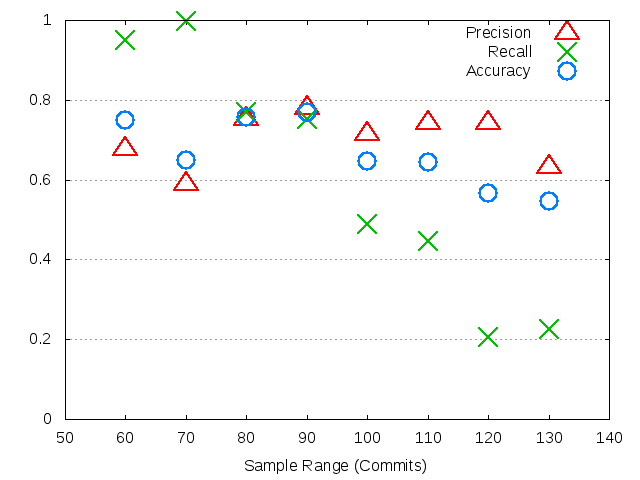
\includegraphics[width=1.0\textwidth]{images/rf/test_1/acra_sample_range}
        \caption{Sample Window Range for acra using RF}
        \label{fig:test_1_acra_rf}
    \end{minipage}
\quad
    \begin{minipage}[b]{0.45\linewidth}
        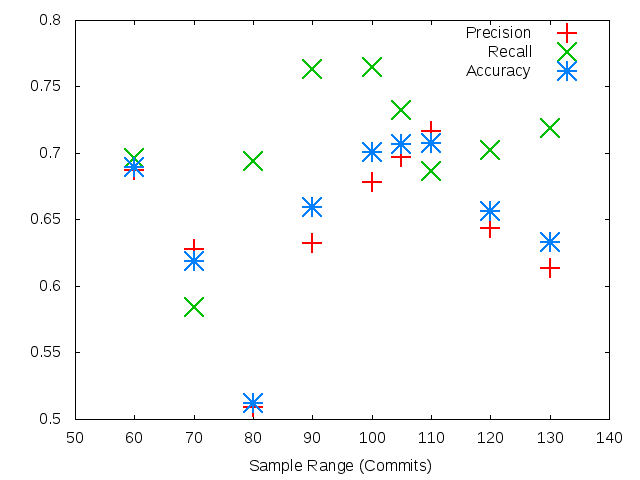
\includegraphics[width=1.0\textwidth]{images/rf/test_1/dagger_sample_range}
        \caption{Sample Window Range for dagger using RF}
        \label{fig:test_1_dagger_rf}
    \end{minipage}
\end{figure}

\begin{figure}[h]
    \centering

    \begin{minipage}[b]{0.45\linewidth}
        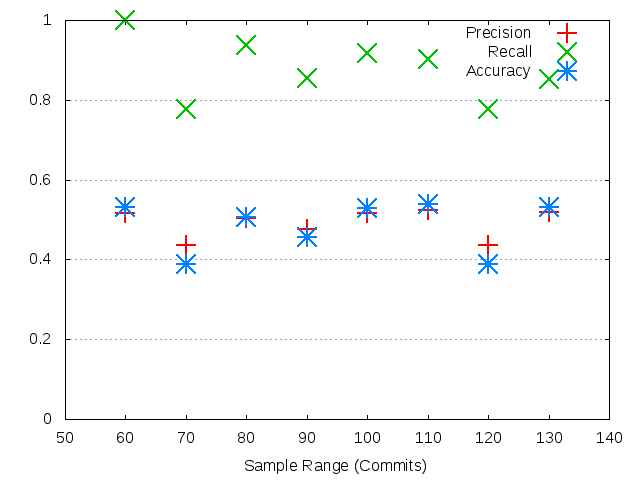
\includegraphics[width=1.0\textwidth]{images/rf/test_1/fresco_sample_range}
        \caption{Sample Window Range for fresco using RF}
        \label{fig:test_1_fresco_rf}
    \end{minipage}
\quad
    \begin{minipage}[b]{0.45\linewidth}
        \includegraphics[width=1.0\textwidth]{images/rf/test_1/storm_sample_range}
        \caption{Sample Window Range for storm using RF}
        \label{fig:test_1_storm_rf}
    \end{minipage}
\end{figure}

\begin{figure}[h]
    \centering
        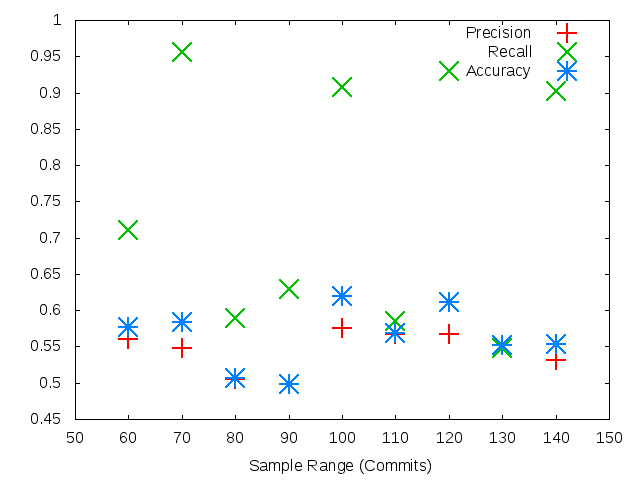
\includegraphics[width=0.45\textwidth]{images/rf/test_1/deeplearning4j_sample_range}
    \caption{Sample Window Range for deeplearning4j using RF}
    \label{fig:test_1_deeplearning4j_rf}
\end{figure}


\subsection{Random Forest Discussion}
\label{subsec:rf_discussion}

%\section{Results}

% TODO re-work this section
% TODO most of this section is out of date and needs to be done.


%%%%%%%%%%%%
% This part is fine.

% Ensure this doesn't overlap to much with the above section which discusses cross-validation.

% TODO remove
%Since the data set is split into four quarters, the category (of whether a method will be changed in the next 5 commits) is known for the first 3 quarters. The final quarter depending on the size the category is also known except for the changes that occur in the last 5 commits. Therefore at project testing data set can be extracted using the feature data and the category for each quarter (except for the last 5 commits of the 4th quarter). One extracted the model can be trained on one quarter at a time and tested on the following quarter.

% \begin{table}
% \begin{center}

%     \begin{tabular}{|l|c|c|c|}
%         \hline
%         Project & Quarter 1 & Quarter 2 & Quarter 3 \\ \hline
%         acra & 0.824 & 0.806 & 0.87   \\ \hline
%         storm & 0.912 & 0.918 & 0.912 \\ \hline
%         %fresco & 0.964 & 0.946 & 0.944 \\ \hline
%     \end{tabular}
%     \caption{Prediction accuracy with sample size of 100}
%     \label{tab:test_signature_change_freq_100}
% \end{center}

% \end{table}

% TODO remove the parts that are incorrect and add in more about the newer experiment results.
%An experiment was run using the feature set of $\{signature, change_i, freq_{change}\}$. The test was run five times with a new random sample each time. The average prediction accuracy of each test was calculated for each project and is shown in \autoref{tab:test_signature_change_freq_100}. The results from the first project are rather standard as numerous other tests were done in order to attempt to find the best feature set for this particular data set. So the particular feature set used performed the best out of all the other feature sets tested. This is just one of the 18 other feature sets that were tested. Of those 19, 8 of them provided a training set which could not be separated and had $43\% \leq P_{accuracy} \leq 68\%$ with an average of $52.7\%$. These prediction scores are fairly abysmal providing on average a very slight advantage over a simple coin toss. Two more of 18 of candidate feature sets were ruled out because they also had a fairly low score of around $52\% \leq P_{accuracy} \leq 77\%$ and an average of $62.6\%$. Finally, the remaining candidate feature sets 8 of the 18 had an accuracy of $72\% \leq P_{accuracy} \leq 90\%$ with an average around $80.8\%$. 

%The top 3 candidates feature sets were tested and proved to have fairly similar results. The set $\{signature, change_i, freq_{change}\}$ was the smallest feature set and also provided the best results and was selected to test on other repositories. This was to test whether the candidate feature set was generally usable or only worked for the test repository \textit{acra}. This feature set was then tested on other GitHub project repositories. The results for the tests involving the other projects are also shown in \autoref{tab:test_signature_change_freq_100}. While an effort was made to optimize the candidate feature set to perform the best on the \textit{acra} dataset the other project's perform even better.

%In particular the project \textit{storm} has a very high prediction score and is much larger than the other two projects shown in \autoref{tab:project_summary}.

%It should be noted that while the \gls{svm} model when trained with a random sample size of 100 performed well, when a sample size of 1000 was used the prediction accuracy was greatly reduced. It would seem that a smaller sample size may prove more helpful regardless of the size of the project. 

% TODO create a table outlining the other combinations.

%%%%%%%%%%%%%%%%%%

%\subsubsection{Detrimental Features}

% TODO rework this stuff, since some of this has been covered earlier on in the experiments section.
% Also the results part has been redone so this part most likely needs it too.

% TODO write about which features were tested and found to not benefit as part of the feature set.
    % - e.g. committer, name.. 
%While initially a larger set of features (the candidate features) was considered, early tests showed poor results and indicated that some of the features may be detrimental. This is not entirely surprising since an \gls{svm} is very dependent on the features fitting within specific requirements outlined earlier in \autoref{subsec:svm_prediction}. Some of the features appeared at first to be acceptable but with further testing and understanding proved to be determinant to the vector in training the model.

%An incrementing unique integer, $commit_id$, was assigned to each commit. Initially this number was used as part of the candidate feature set. However further investigation determined $commit_id$ would only negatively affect the results. Given that each commit was provided a unique incrementing value only methods changed in the same commit would be given the same number. While this may seem initially useful tests showed the opposite. % TODO cite experimental data showing such.

%Other candidate features that were tested more extensively also proved to have a poor effect on the \gls{svm} model. The candidate features that appeared to have a negative impact on the \gls{svm} model were $committer$, $change_{prev}$, $\Delta t$. The fact that these features had a negative impact does not necessary mean that they are unrelated to the changes that occur to methods. However, in conjunction with other candidate features the model created consistently made inaccurate predictions.

%\subsubsection{Valuable Features}

% While the previous candidate features performed poorly, candidate features $signature$, $change_i$, $freq_{change}$ and $name$ all were apart of feature sets that performed very well. 

% $name$ was found to not have a large impact and slight detrimental impact on performance but while included still achieved a rather high prediction score. 

%features $signature$, $change_i$ and $freq_{change}$
% test_signature-change-freq sample size 100

% TODO add histogram of work.
%\chapter{Literature Review}
\label{chap:related_works}


\section{Data Mining}

Data collection from some original source provides access to a data set that may not be initially available. This data source could also be in a state that is not convenient or feasible for use without leveraging data mining techniques to transform the data to a more accessible state. The source of the data can vary greatly based on the interests for the individual(s) collecting the data. Data mining has mostly focused on single source mining and multiple data sources. Data mining in general has however also taken a large focus on data collection from software repositories which can be either single or multiple source \cite{Hemmati2013}, \cite{Hassan2006}, ... %TODO list other msr based papers.
% TODO find other work of data mining

% MSR, guiding future changes
Zimmermann et al. map the changes that certain developers make and who change certain functions to the functions they also change \cite{Zimmermann2005a}. 

% Change analysis
Maletic and Collard investigate changes with a software project's development cycle. The changes are extracted and stored in an more easily usable representation \cite{Maletic2004}.

% MSR Change extraction of changes
Canfora et al. propose a method for extracting and refining the changes made throughout the life a project to be used in more effective analyses \cite{Canfora2007c}.

Hemmati et al. take a comprehensive look at the research related to \gls{msr} to determine best practices and point towards future work \cite{Hemmati2013}.

% MSR in general
Hassan cover the different metrics and uses of \gls{msr} \cite{Hassan2006}.

% Validation of Change history research, benchmark
Dit et al. provide a benchmark dataset to help in the testing and comparing of various methods for improving software maintenance tasks \cite{Dit2013}.

% TODO MERGE this with related work
\subsection{Mining Open Source Software Repositories}

% TODO ensure this is accurate.
\gls{oss} generally is software that provides with the ability access the source code and make modifications to the source code. While certain licenses provide some restrictions on the ability to redistribute the software the main point of the source code of the software being freely available is key. The scope and capability of \gls{oss} projects vary greatly. Several very popular \gls{oss} projects are listed in table \ref{tab:oss_projects}.

%TODO make sure footnotes fit in better.
\begin{table}[h!]
\begin{minipage}{\textwidth}
\begin{center}
    \begin{tabular}{|l|l|l|}
        \hline
        Owner & Project & Description \\
        \hline
        Mozilla & Firefox\footnote{\url{https://www.mozilla.org/en-US/firefox/desktop/}} & Internet Browser \\
        Linux & Linux Kernel\footnote{\url{https://www.kernel.org/}} & Operation System Kernel \\
        VideoLAN & VLC\footnote{\url{http://www.videolan.org/vlc/index.html}} & Media Player \\
        PostgreSQL & PostgreSQL\footnote{\url{http://www.postgresql.org/}} & Object-Relational Database Management System \\
        git & git\footnote{\url{https://git-scm.com/}} & Version Control System \\
        \hline
    \end{tabular}
\end{center}
\caption{Open Source Software Projects}
\label{tab:oss_projects}
\end{minipage}
\end{table}
%Firefox => MPL 2.0
%Linux Kernel => GPL v2, plus various closed-source binary blobs
%VLC => GPLv2+ (player), LGPLv2.1+ (engine)
%PostgreSQL => PostgreSQL License
%git => GNU General Public License v2, GNU Lesser General Public License 2.1

The development of large software projects (whether \gls{oss} or not) often make use of \gls{vcs}. A \gls{vcs} helps the developers of the project manage the changes of the project and facilitate the collaboration between developers. A \gls{vcs} will keep an current version of the project and keep track of the previous version of the project as well. This may be done through keeping a copy of each version of the project or by keeping track of all each change made to the project. \gls{svn} and git would be two examples of \gls{vcs}s.

Git is a \gls{dvcs} and differs greatly from \gls{svn} which is a normal \gls{vcs}. Git will provide the user with a complete copy of the repository that is worked on independent of network connection. The independence of each repository also allows for a repository to be developed without a centralized server. The distributed aspect of git tends to allows for easier use for all involved parities. The one main issue with a \gls{dvcs} is that while decentralization is useful, developers will require some method to collaborate and communicate to transfer changes made to the repository. Therefore typically one centralized server is used to maintain communication between all interested parties.

Git has grown in popularity since it was created and is at the core of several \gls{vcm} sites such as GitHub \footnote{\url{https://github.com/}}, BitBucket \footnote{\url{https://bitbucket.org/}} and GitLab \footnote{\url{https://gitlab.com/}}. These platforms tend to be fairly supportive of \gls{oss} projects through providing their services free of charge. For example, GitHub provides unlimited public repositories completely free. While these projects do not have to be licensed with an open source license typically they will be since they are already publicly visible.

% GitLab -> https://gitlab.com/
% GitHub -> https://github.com/
% BitBucket -> https://bitbucket.org/

GitHub is the most popular of the \gls{vcm} websites and hosts numerous very popular \gls{oss} projects including, the Linus Kernel, Swift\footnote{\url{https://swift.org/}} and React\footnote{\url{https://facebook.github.io/react/}}. GitHub also provides a public \gls{api} to allow for access to the data related to project repositories which is discussed further below. % TODO link to that.
Given the popularity of GitHub for use by developers and the availability of the project data, GitHub is an obvious choice for mining project data. Especially since the goal of mining software is to capture \gls{oss} project data to both explore and test analysis methods. Publicly visible projects are also publicly accessible through the \gls{api} and the majority are open source.

%%%%%%%%%%

Git provides a simple interface to manage the repository regardless of which site is the central server. Therefore regardless which site the project resides on users can easily interact with the project as long as they know the git interface. Git in essences is a file storage for the project that keeps track of changes made to the project. A \textit{commit} is a set of changes that a developer has made at a certain time. The developer has full control what gets committed, when it gets committed and even modified at a later date.
%This results in the date of the commit merely identifying when the developer formally notified Git that a change was made.

A branch is a series of commits that are often related. In figure \ref{fig:network_diagram}, each dot would represent a commit and a set of dots connected by the same colored lines are a branch. Branches can be considered different paths or deviations in the development from each other allowing for different versions of the project to be maintained and developed. The \textit{master} branch is the main branch, represented with black, from which all branches usually stem from and is generally where projects are developed on. On a similar note, a \textit{tag} is a branch that is frozen to allow for future reference. Tags are often uses to mark a significant point in the development history such as a project release. Finally, when two differently branches converge into a single dot then the two branches have been \textit{merged}. A merge indicates that the differences between the two branches are consolidated based on the developer's discretion.

\begin{figure}[!ht]
    \centering
        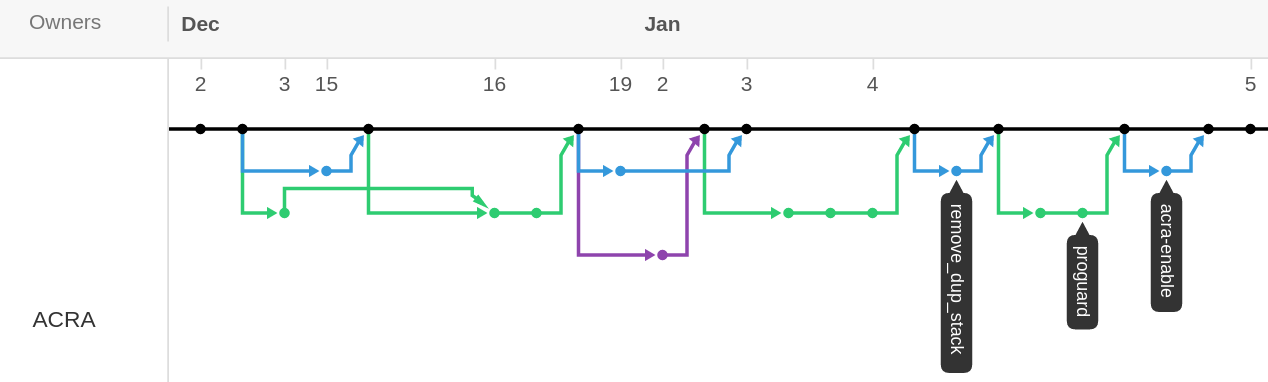
\includegraphics[width=1.0\textwidth]{images/network}
    \caption{Network diagrams}
    \label{fig:network_diagram}
\end{figure}

A commit consists of files that have been changed, more specifically a list of \textit{patch} files which each outline the changes made to their corresponding file. The patch file consists of a series of differences between the previous version of the file and this new version of the file. These patch files are key since they contain the actual changes made to the project and thus are the major point of interest.

% TODO fix close

\section{Machine Learning}

% Rase, realizing software engineering learning
Machine learning is a complex method for software algorithms to attempt to determine patterns within the data. One such problem example would be an algorithm to detect certain people within an image. For an individual such a task may seem trivial however for a software system to detect it is far more difficult. Algorithms that can determine patterns and mimic them from abstract set of data is useful when such patterns are extremely complex. There are numerous algorithms which apply machine learning approaches. Each approach has both advantages or disadvantages. Some examples of machine learning algorithms are \gls{svm}, \gls{rf} and \gls{ann}. The three provided examples are also commonly used for data mining \cite{Alam2013}, \cite{Granitto2007}, \cite{Westland2011}, \cite{Yu2011}, \cite{Huang2007}, \cite{Jalbert2012} %TODO get some papers for svm and ann

Bhattacharyya et al. provide a detailed description of \gls{rf} and \gls{svm}.

\subsection{Support Vector Machines}
\label{subsec:svm_prediction}

\gls{svm} models are more easily modified to fit data from different sources since they flexible and robust than more classical linear regression models *cite*. %TODO consider citing 

A \gls{svm} is used to predict what type of change will occur based on a set of features provided. A feature is a data extracted from the project represented as a floating point number. In order to be useful a feature must in some way characterize the the category that it is assigned to. The feature must also not rely on the category that it belongs to in order to be calculated. For example, given a category of the method change within the next 5 commits or not, then the features must not rely on knowledge of future changes to the project. If the features fail to effectively characterize the category they are assigned to then the \gls{svm} may have poor predictions. It is also necessary for the features to independent of each other to not negatively affect the categorization.


\gls{svm} has been widely used for making predictions for various aspects including predicting battery charge state \cite{Anton2013}, pharmaceutical data \cite{Burbidge2001}, software faults \cite{Gondra2008, Erturk2015, Malhotra2015, Kim2008, Moeyersoms2015, Neuhaus2007}, bug localization \cite{Murphy2007, Neuhaus2007}, software mutation testing score \cite{Jalbert2012}, financial stocks \cite{Kim2003}, credit score \cite{Huang2007}, credit card fraud \cite{Westland2011}, solar power output \cite{Zeng2016}.

Malhotra reviews numerous machine learning techniques, including \gls{svm} and \gls{rf}, used by various studies. The results of which outline where each approaches succeed and falls short. When using a machine learning algorithm it is imperative to use a suitable algorithm for current situation. Kim et al. outline a approach that uses a \gls{svm} to predict changes that will occur within the project. By identifying these changes the a project developer can potentially locate a bug within a change and fix it prior to being reported. Erturk and Sezer compare the performance of their proposed method, an Adaptive Neuro Fuzzy Inference System, to that of an \gls{svm} for predicting software faults. The models are trained using project metrics as well as the project's historical fault data. Zeng and Qiao use a \gls{svm} to provide short-term predict solar power output. The \gls{svm} model outperformed both an autoregressive and a neural network model. Anton et al. propose a method for predicting the state of charge of a battery using \gls{svm} model.

Bhattacharyya et al. uses \gls{rf}, \gls{svm}, logistic regression to detect credit card fraud. Both \gls{rf} and \gls{svm} are able to predict a large number of fraudulent credit card transactions.


% TODO talk even more about how to pick better features.
%<<< TODO Example feature vector >>>

% \begin{table}
% \begin{center}
%     \begin{tabular}{|l l l l l l l|l|}
%         \hline
        
%         Features &  &  &  &  &  &  & Description \\
%         \hline
%         $name$ & $signature$ & $change_i$ & $committer$ & $freq_{change}$ & $change_{prev}$ & $t_\Delta$ & $change_{next\_6}$ \\
%         %0.0 & 0.1 & 0.0\\
%         \hline
%     \end{tabular}
% \end{center}
% \caption{Example Feature Vector}
% \label{tab:example_feature_vector}
% \end{table}

% TODO Format parts of this.
\gls{svm} requires all feature data be encoded as floating point numbers. For any numerical data the conversion to floating point is trivial. However, for more complex data the conversion is a little more difficult. Categorical data can be mapped into a unique vector entry per category. For example, if a feature can be 1 of 3 options: 0, 1 or 2 then it can be converted into three entries in the feature vector. Encoding the value 2 the sub-vector of the feature set would be [0, 0, 1] where 1 indicates a field that feature is present in the data for this vector, and 0 indicates the feature is not present. Data that is in the form of a string can be converted to a floating point number by assigning a unique number for each string (similar to hashing). The one downside to this method is that the numbers corresponding to each string maintain no numerical properties. In essence the data becomes categorical, such that if \textit{bob} is mapped to 1 and \textit{sally} is mapped to 2 there is no relationship between 1 and 2. Ideally, this data would then be further converted using the previously described method however if the set of possible strings is large then it may be unreasonable to convert it. For example, if there are 100 possible strings then that would add 100 new entries to a single vector.

%<<< TODO svm diagrams >>>

The categorization is used for the prediction, where each value of the category relates to a unique prediction type. For example, a simple binary categorization could simply 1 or 0 where 1 predicts the event will occur and 0 predicts that the event will not occur. In essence an \gls{svm} is tasked with separating a dataset into two different categories given a sample set of data that has already been categorized into two subsets. Given the categorization of the sample dataset the \gls{svm} model is trained to allow for categorization of new data. The categorization of any new vectors (that were not used for training) is called a prediction and is made by the \gls{svm} model created through the training. More specifically, the sample dataset is a dataset extracted from the target dataset. The sample dataset is then categorized based on the predetermined criteria (the prediction goal). This dataset along with the categorization for each vector in the dataset is the training dataset, and is then used to \textit{train} the \gls{svm} model. Once the model has been trained, the \gls{svm} model is ready to be used for making classification predictions. The data for each feature can be extracted from the new dataset, allowing for the model to classify each new vector. Given that the \gls{svm} model is accurate and reliable the results can then be used towards making predictions about the dataset. For example if the classification is that of predicting change to occur within the next six commits the developer may wish to be careful with the use of the method or assess the method's quality and determine if any issues within the method need to be addressed.

A lower prediction score often relates to the data from the feature set poorly characterizing the categories. Similarly a warning will be given if the dataset is in-separate. In this case, the dataset for each category may be too similar and cannot be properly split into the two category subsets. In both cases a change to the feature set may help, whether that is a decrease or increase of features in the set. Some features are detrimental to the model, especially two features related to one another. Other potential steps would be to modify the data to ...
% *** TODO determine best practices for data something like mean of 1 and std of 1. ***

More details about the specific features used will be given a little later on. Features are descriptive aspects of the dataset that are classified into the predetermined categories. Since these features relate directly to the category understanding of the classification critical and can help determine which features should be used. For example for a classification of whether a change will occur within the next few commits, a useful feature may be the frequency by which a method changes within the project. Picking a descriptive feature set is paramount to providing a strong prediction of future data.

%<<< TODO create a figure to outline the various features and their meaning >>>

Most of this was done using database queries or user defined functions created in the database language.

% TODO get some papers related to support vector machines.

\subsection{Random Forests}
\label{subsec:random_forest_predictions}

\gls{rf} are a popular machine learning algorithm and is used in numerous areas including predictions for software fault \cite{Malhotra2015, Moeyersoms2015, Guo2004}, software development effort \cite{Moeyersoms2015}, credit card fraud \cite{Westland2011}, database indexing \cite{Yu2011}, malware detection \cite{Alam2013}. 

Malhotra provides an extensive review of studies involving machine learning to predict software faults. The results showed that \gls{rf} tended to preform better than other machine learning algorithms studied. Moeyersoms et al. made use of \gls{rf} and \gls{svm} as well as a few other data mining approaches to predict software faults and effort estimation. The data mining techniques are used as part of another model, ALPA rule extraction, to improve the predictions and increase traceability. Guo et al. attempt use \gls{rf} to predict the fault proneness of modules within a project. The \gls{rf} prediction results for the five sample projects prove more accurate to that of a logistic regression. Yu et al. attempt to use \gls{rf} to determine a more effective database indexing for video data. The database index are used to provide faster searching of the database for action detection.

\gls{rf}s are commonly used to on data that has been mined from some source to make predictions \cite{Alam2013}, \cite{Granitto2007}, \cite{Yu2011}. A \gls{rf} leverages numerous decision trees to provide attempt to improve prediction capabilities. Therefore to fully understand a \gls{rf} first an understanding of decision trees is necessary. A decision tree is a technique which will create a tree based on a data set that has been classified. Once the decision tree model is created it can be used to predict or categorize data that has not yet to be classified. In the tree model the leafs will be categorizations where as the connections between inner nodes are the decisions by which the categorizations are made.

% TODO format
One issue with decisions trees and more generally machine learning techniques in general is imbalanced data sets for training the model \cite{Khoshgoftaar2007}. The data set used rarely provided even sample sizes of each set therefore without taking necessary pro-cautions the algorithm will bias the results. In the worse case the model will classify any input data as the larger data classification.

In case of imbalanced datasets there are several methods to help provide stronger predictions \cite{Khoshgoftaar2007}. The most obvious and easiest to attempt would be to sample more data. However if the dataset in general follows this trend then some more advanced techniques can used to improve the model.

% Note when remarking about model quality this refers to accuracy and recall of the model
 
The first method would be to \textit{undersample} larger category this will even out both of the categories. This will remove some of the input values within the dataset to reduce the set size. However if there are very few samples of the smaller category the performance will suffer as well. A second method of \textit{oversampling} is useful in the case were the data samples are small. The input data from the smaller category is selected to be duplicated in the set to increase the size of the set. This helpful since it will increase the size of the dataset but could lead to bias based on the data selected from the smaller dataset. The selection method for which input vectors to over or under sample can be based off on the data's statistical distribution or made by random choice. Another advantage of these over and under sampling is that they can also be used together to in the case of a large disparity between the category's set size. 

% Bootstrapping aggregation
Another feature of \gls{rf} which is used to help provide more reliable predictions is \textit{Bootstrap Aggregation} \cite{Westland2011}. Similar to normal sampling methods it will take the initial dataset. However rather than using the dataset as is the dataset will be uniformly sampled $n$ times and repeated $m$ times to create $m$ datasets of $n$ values. These newly created datasets will then be used to train $m$ models. Finally, when attempting to categorize a new input data it will be given to every model and the prediction result will be aggregated to provide a more accurate results. For some machine learning methods such as \gls{svm} this method will improve the results and help with imbalanced datasets.

A \gls{rf} is a collection of decisions trees trained on random samples of the initial dataset. So the \gls{rf} will take an input dataset and then train $m$ decisions trees using $m$ randomly sampled sub-datasets of the initial dataset. This helps improve the model created and makes \gls{rf}s far easier to use. As well \gls{rf}s have a feature that determines the importance of each feature is assessed during the training of the model \cite{Westland2011}. The importance outlines the quality of each feature in providing the prediction \cite{Verikas2011}. Therefore in order to properly understand the feature importance the accuracy, precision and recall of the model should be determined by running a test dataset to determine the quality of the model.

\section{Software Development Prediction}
% TODO actually write about each of the papers.

%TODO work this together 
Software development prediction contains numerous areas of study which generally attempt to improve projects by focusing on their development and providing feedback to the developers through predictions. Some of these areas include, fault detection \cite{Nagappan2007, Moser2008, Thwin2005, Sisman2012}, mutation score \cite{Jalbert2012}. While there may be a large overlap in the objective for these studies often they will vary in what is used to make the prediction.

% Close source, prediction
%Nagappan and Ball use the software dependencies and churn metrics to predict the failure of a commercial product post release \cite{Nagappan2007}.

% Defect prediction, change attributes, static attributes
%Change and static code attributes are compared in their capability in predicting defects within a project \cite{Moser2008}.

% predict software quality based on code metrics
%Attempt to predict the number of defects within a given class using a neural network trained on object oriented code metrics \cite{Thwin2005}. Second the amount of changes within a class is predicted again with a neural network using object oriented code metrics \cite{Thwin2005}.

% Prediction of something
%Support development of software predictions is a common research area. Jalbert and Bradbury used static metrics from both the source code and corresponding test suites to predict the mutation score for the test suite \cite{Jalbert2012}.

% Bug localization through prediction, change history, defect history, temporal decay.
%Sisman and Kak leverage defect history and the change history of a project to predict which files will be the cause of bugs in different version of the project \cite{Sisman2012}.

\subsection{Change Prediction}
% Related work stuff here or later

The development of large scale projects can take a long time and involve a huge time investment from the developers. The development of the project will cause for the developers to make changes to projects. Software projects will have faults within the project especially during the development phase. A project in its early stages may not meet the full set of functionality since it has not been completed yet. Since the development team will known that such features are not yet implemented these faults or fails are not a huge concern. Rather faults that are unknown to the developer team are far more serious. Such cases as a feature was thought to be implemented correct but was not or a feature implementation breaks other features. In both those cases changes made to the project cause the fault to be revealed.

Changes to the project are the means by which all development occurs. The ability to analyze and predict changes within a project could give deep insights into the development of a project.


A large amount of research as focused on predictions of changes based on changes \cite{Bantelay2013}, \cite{Chaturvedi2014}, \cite{Giger2012}, \cite{Hassan2004}, \cite{Kagdi2007}, \cite{Ying2004}. 

Ying et al. present a method that predicts which parts of the system will change given a set of changes \cite{Ying2004}. The prediction method leverages the change history.

Kagdi and Maletic also leverage version history changes to perform software change predictions \cite{Kagdi2007}. The actually analysis applied is two fold, through the dependency analysis of the current version and the change analysis of the version history. The data is collected through \gls{msr} which is a popular field of study. 

In a similar work, Hassan and Holt, worked towards predicting change propagation of a given initial change. \cite{Hassan2004} The main question was to determine given a change to an entity (e.g. function or variable) will propagate to changes in other entities. This work is very related since it tests various methods and leverages presents the best one.

Bantelay et al. propose a method that mines the file and method level evolutionary couplings to attempt to predict commits and other interactions within the project \cite{Bantelay2013}. Both methods were used in isolation as well to determine whether the attributes were more helpful when used together.

Giger et al. attempt to build off of previous work in change prediction (proneness) by providing predictions relating to more refined entities \cite{Giger2012}. The syntax changes are recorded but an attempt is made to capture semantic changes on the statement level \cite{Giger2012}.

Chaturvedi et al. attempt to predict the complexity of the project given it's change history using an entropy analysis \cite{Chaturvedi2014}.

% Change prediction (proneness), visualization
Further work in change analysis was done by Bieman et al. in studying the change-proneness of different entities within a software project \cite{Bieman2003}. In order to provide a deeper understanding visualizations were used as well providing a bit of a different approach from some of the other works.

% Change prediction (proneness)
Koru and Liu study and describe change-prone classes found within open source projects \cite{GunesKoru2007}.

% impact of changes aka precursor to predicting changes. Providing a type of rudimentary prediction by taxonomy.
Wilkerson attempts to classify different types of changes that occur to a project throughout its development \cite{Wilkerson2012}. The classification can then be used to identify the impact that a given change will have on other aspects of the project.

% (TODO check) Close source, identifying areas likely to have change
Snipes et al. describe a tool for analyzing software projects to identify areas that have a history of large amount of change. \cite{Snipes2011}






% TODO talk about previous work on change prediction. cause. 

%There are several different areas of study that are related to this work. Some are more closely related than others and will receive more attention accordingly. A quick summary of the fields that are related are as follows: 

% TODO run libsvm analysis on best candidate feature set.

% TODO work on.
% - Data Mining
%   - MSR is a great place for these types of works.
% - Repository/Version History analysis
%   - Analyzing the changes made to the project to some end.
% - Prediction systems
%   - Change prediction
%   - Predicting whether change will occur or which changes will occur given using some data set.

%21/20-25

% Change Prediction, version history as resource

% \begin{table}
% \begin{center}
%     \begin{tabular}{|l|l|l|l|l|l|}
%         \hline
%         Author & AI Technique & Source & Data & Goal & Accuracy \\
%         \hline
%         Ying et al. & N/A - Uses previous changes & CVS & Change Patterns & Related source code that should change & Mozilla: \{ P:50\% R:20\%-30\% \} Eclipse: \{ P:30\% R:10\%-20\% \} \\
%         Kagdi and Maletic & N/A - Impact Analysis & SVN & Current and historical dependencies & Software change & N/A \\
%         Hassan and Holt & Heuristics & CVS and Perforce & Change History & (Varies) Developer Co-Changes and Entity Co-Change and Entity Co-Call Use Define (CUD) and Entity Co-Change File & Accuracy \\
%         \hline
%     \end{tabular}
% \end{center}
% \caption{Experiment projects}
% \label{tab:project_summary}
% \end{table}



% ~ denotes an approximation based on a graph.
%  ** Best performance

% Author & AI Technique & Source & Data & Goal & Accuracy

% Ying et al. & N/A - Uses previous changes & CVS & Change Patterns & Related source code that should change & Mozilla: { Precision: 0.50, Recall: 0.20-0.30} Eclipse: { Precision: 0.30 Recall: 0.10-0.20 }

% Kagdi and Maletic & N/A - Impact Analysis & SVN & Current and historical dependencies & Software change & N/A

% Hassan and Holt & Heuristics & CVS and Perforce & Change History & (Several Methods) Developer Co-Changes (DEV), History Entity Co-Change (HIS), Entity Co-Call Use Define (CUD), Entity Co-Change File (FIL) and Hybrid (HYB) & DEV: {Precision: 0.01, Recall: 0.74 }, HIS { Precision: 0.06, Recall: 0.87 }, CUD { Precision: 0.02, Recall: 0.42}, FIL { Precision: 0.12, Recall: 0.83 }, HYB(80, 10) { Precision: 0.49, Recall: 0.51 }**, HYV(80,30) { Precision: 0.35~, Recall: 0.65~ } HYB(60,30) { Precision: 0.25~, Recall: 0.75~ } & Very Related

% Bantelay et al. & Impact Analysis & Mylyn and CVS & Interactions (through Mylyn) and commit history and relationships (CVS) & Commit Prediction

% Thwin and Quah & Neural Networks (Ward Neural Network and General Regression Neural Network (GRNN)) & Source Code (Static Analysis from Project) & Object Oriented static metrics (inheritance, complexity, cohesion, coupling and memory metrics) & 1: Number of defects in a class, 2: number of lines changed per class & Correlation is tested rather than accuracy. 1: (R^2: 0.88, r: 0.94; R^2: 0.86: r: 0.94) 2: (R^2: 0.71, r: 0.86; R^2: 0.56, 0.76)


% Jalbert & Support Vector Machine & Source Code (Static Analysis from Project) & source code static metrics and test suite static metrics & predict test suite mutation score & approx 0.71

\chapter{Conclusions}
\label{chap:conclusions}

\section{Summary}

We proposed a method that leverages the commit history to predict future changes within the repository. The data used for predictions was collected from \gls{oss} repositories on GitHub. The data was then visualized through several techniques to help identify key features for use in the prediction model. The features were selected and a model was created to predict whether change will occur in the short term of 5 commits. Three experiments were conducted on the approach using 23 different \gls{oss} repositories developed in Java. The experiments investigated the three different factors; sampling range, model features and data set balancing to identify measure the impact on the performance of the approach. The results of the experiments show that while the \gls{swr} had a strong impact on the performance, the repositories themselves often had internal factors which caused differences in performance.

\section{Contributions}

The contributions of this work are:
\begin{enumerate}
\item Determined which factors more strongly influence the performance of the predictions approach.
\item Out of the three factors investigated, the \gls{swr} proved to have the greatest impact for both \gls{svm} and \gls{rf}.
\item Providing an approach that with some success can predict future changes within a repository using the commit data. Both \gls{svm} and \gls{rf} are viable for a few repositories such as acra, http-request and ShowcaseView.
\end{enumerate}

\section{Limitations}

%http://dissertation.laerd.com/how-to-structure-the-research-limitations-section-of-your-dissertation.php
%http://dissertation.laerd.com/what-readers-expect-from-the-research-limitations-section-of-your-dissertation.php
%http://www.sicotests.com/darticle.asp?page=238

The limitations placed on this approach often are divided into two categories; limitations used to simplify the approach and limitations inherent to the approach. The limitations used to simplify the approach are:
\begin{itemize}
\item Repositories are required to have a commit size of $300 < c < 4000$. The lower bound helped prevent experimentation on very small repositories which would not have had enough data. Likewise the upper bound helped restrict experimentation on huge repositories which will take longer to train and provide a more difficult challenge when modeling change.
\item Repositories must consist of at least $75\%$ Java source code. The prediction model feature collection process required identifying language specific details and would require a reimplementation for any new language.
\item Repositories had to be developed on GitHub and openly available. Since the goal was to extract the data from an entire repository the availability was essential. GitHub provides an easy to use interface for collecting repository data and used to collect the data. Another method for collection or another source could be devised as long as the method collects the necessary data and the source provides the necessary data.
\end{itemize}
While some of these restrictions are easily circumvented some are also inherent to the implementation. For example the second two would require fairly substantial reimplementation to overcome these limitations. These are however possible since creating a method for collecting from different sources would open the approach to more repositories and allow for further use. Likewise, implementations done in other languages would allow for more repositories to make use this approach.

% - mitigating project internal factors causing differences between projects
% 	- projects can't be compared as easily
% 	- approach requires tailoring for each project. Aka no generalizable solution
% - No guarantees about the good solution found will be the best.
% 	- A guide is provided to help you find a good solution path (not the best).
% - In order to achieve good results for throughout the life of a repository the parameters will likely require tunning over the life of the Repository
%	- Repository development will change over time. Its very unlikely for the prediction model (even if a new model is created) will work effectively with the same parameters. Some of the experimentation done throughout the development of this approach showed as much.
The other set of limitations outlines ones that are internal to the approach and are only discovered through experimentation. These limitations are:
\begin{itemize}
\item Repository internal factors play a large role in how well the repository performs. The experimental results showed that while some repositories may perform well others classified similarly will perform very differently. These factors were not effectively controlled by the parameters and therefore the results are unpredictable.
\item Finding the optimal set of parameters for creating the prediction model is very difficult since these parameters will vary per repository. The extend of the impact of the parameters while investigated was not fully quantified. Therefore in order to find a better solution for a given repository tunning of the parameters is necessary. Finally, while a good solution may be found better solutions may be available but difficult to find.
\item The prediction model is very sensitive to differences within a given repository which is easily shown in the variation between repository results for a given set of parameters. Therefore the ideal parameters for a given repository are only ideal for the current section of the data set investigated.
\end{itemize}
% TODO discuss how these can be mitigated and address in the future.

\section{Future Work}

% TODO add more future work
Future work includes investigating the repositories and they differ in the way they change. The four repositories that tended to do will together were acra, ShowcaseView, http-request and ion which also shared similar repository characteristics. Finally a more extensive look at the other factors that were involved in the approach to determine their impact of the approach.

% TODO:
% - summary
% - contribution
%     - restated, in more depth
% - limitations
%     - Based around using GitHub data set
%     - as well as limited data from git and open source
% - future work
% - conclusion section
%     - summarize what we've done, what can we really learn about prediction and our our approach
%     - how does this compare to results we've archived version other methods


% TODO 
% either talk about this here, or in the dicussions section of the rf and svm experiments.
% - limited range of swr, wasn't exhaustive.
% - limited set of factors, wasn't exhaustive.

\appendix
\chapter{Experimental Data}
\label{app:experimental_data}

\section{Experiment 1}
\label{app_sec:experiment_1}

\subsection{Support Vector Machine}
\label{app_sub:experiment_1_svm}
% params: test_1, svm

% Figure for \gls{swr} for acra using \gls{svm}
\begin{figure}
\centering
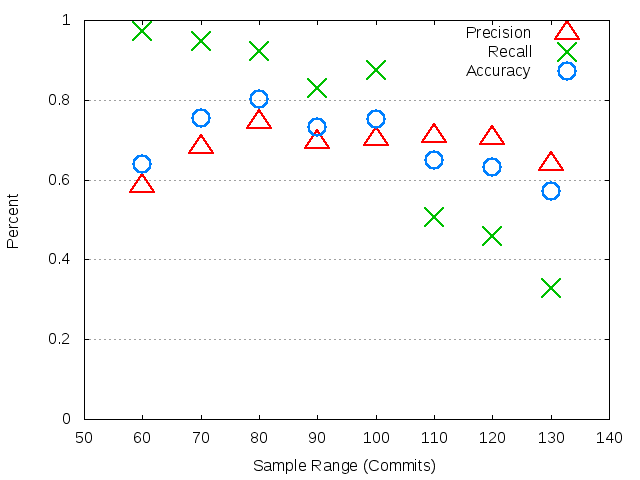
\includegraphics[width=0.8\textwidth]{images/svm/test_1/acra_sample_range.png}
\caption{\gls{swr} for acra using \gls{svm}}
\label{fig:test_1_acra_svm}
\end{figure}

% Figure for \gls{swr} for arquillian-core using \gls{svm}
\begin{figure}
\centering
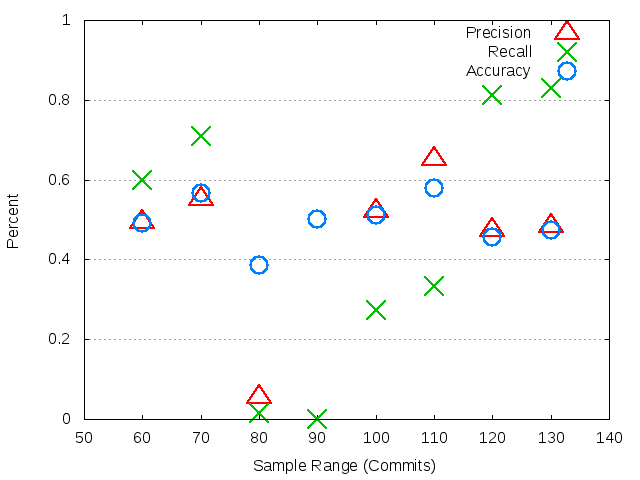
\includegraphics[width=0.8\textwidth]{images/svm/test_1/arquillian-core_sample_range.png}
\caption{\gls{swr} for arquillian-core using \gls{svm}}
\label{fig:test_1_arquillian-core_svm}
\end{figure}

\clearpage

% Figure for \gls{swr} for blockly-android using \gls{svm}
\begin{figure}[!t]
\centering
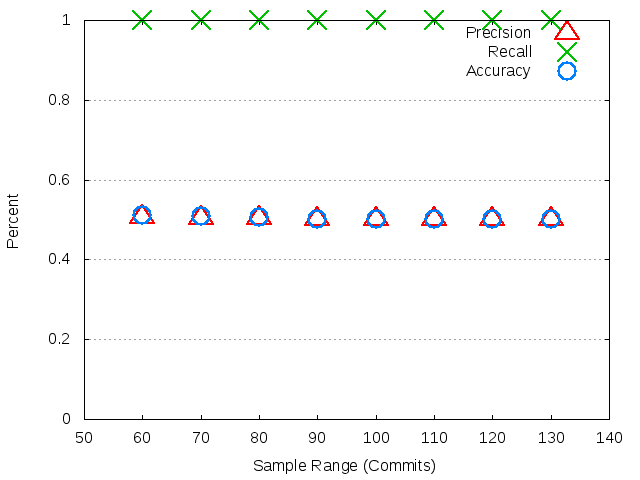
\includegraphics[width=0.8\textwidth]{images/svm/test_1/blockly-android_sample_range.png}
\caption{\gls{swr} for blockly-android using \gls{svm}}
\label{fig:test_1_blockly-android_svm}
\end{figure}

% Figure for \gls{swr} for brave using \gls{svm}
\begin{figure}[!t]
\centering
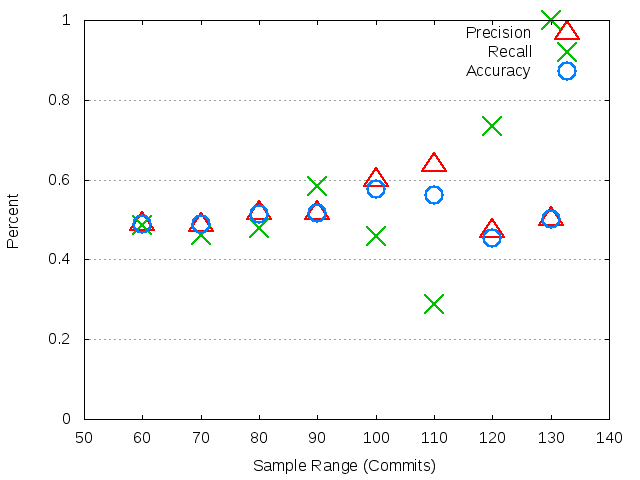
\includegraphics[width=0.8\textwidth]{images/svm/test_1/brave_sample_range.png}
\caption{\gls{swr} for brave using \gls{svm}}
\label{fig:test_1_brave_svm}
\end{figure}

% Figure for \gls{swr} for cardslib using \gls{svm}
\begin{figure}[!t]
\centering
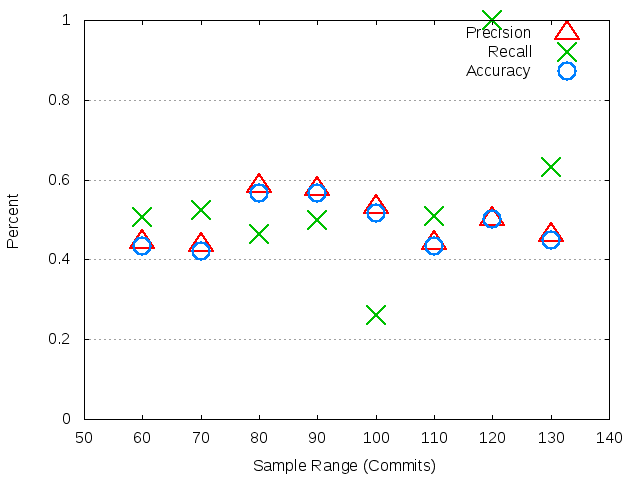
\includegraphics[width=0.8\textwidth]{images/svm/test_1/cardslib_sample_range.png}
\caption{\gls{swr} for cardslib using \gls{svm}}
\label{fig:test_1_cardslib_svm}
\end{figure}

% Figure for \gls{swr} for dagger using \gls{svm}
\begin{figure}[!t]
\centering
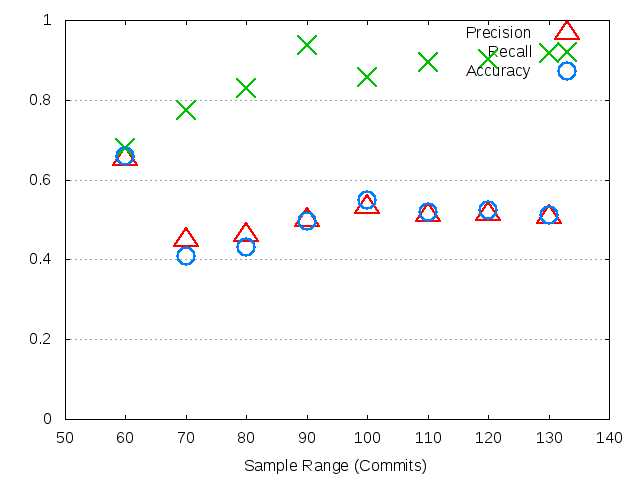
\includegraphics[width=0.8\textwidth]{images/svm/test_1/dagger_sample_range.png}
\caption{\gls{swr} for dagger using \gls{svm}}
\label{fig:test_1_dagger_svm}
\end{figure}

% Figure for \gls{swr} for deeplearning4j using \gls{svm}
\begin{figure}[!t]
\centering
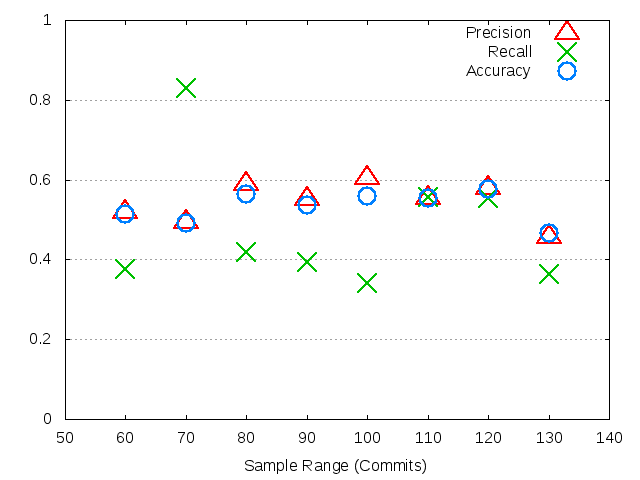
\includegraphics[width=0.8\textwidth]{images/svm/test_1/deeplearning4j_sample_range.png}
\caption{\gls{swr} for deeplearning4j using \gls{svm}}
\label{fig:test_1_deeplearning4j_svm}
\end{figure}

% Figure for \gls{swr} for fresco using \gls{svm}
\begin{figure}[!t]
\centering
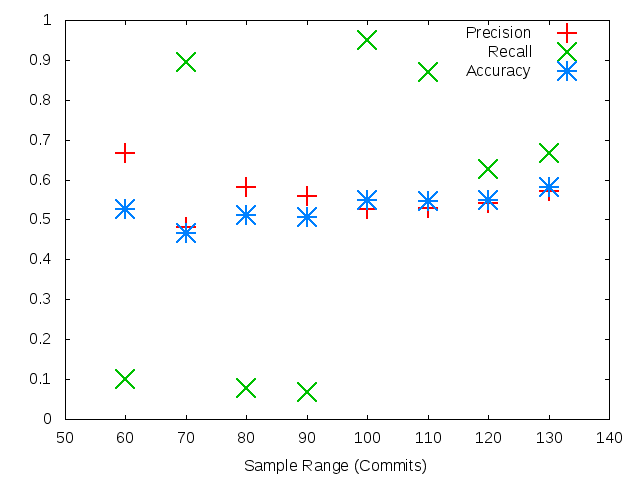
\includegraphics[width=0.8\textwidth]{images/svm/test_1/fresco_sample_range.png}
\caption{\gls{swr} for fresco using \gls{svm}}
\label{fig:test_1_fresco_svm}
\end{figure}

% Figure for \gls{swr} for governator using \gls{svm}
\begin{figure}[!t]
\centering
\includegraphics[width=0.8\textwidth]{images/svm/test_1/governator_sample_range.png}
\caption{\gls{swr} for governator using \gls{svm}}
\label{fig:test_1_governator_svm}
\end{figure}

% Figure for \gls{swr} for greenDAO using \gls{svm}
\begin{figure}[!t]
\centering
\includegraphics[width=0.8\textwidth]{images/svm/test_1/greenDAO_sample_range.png}
\caption{\gls{swr} for greenDAO using \gls{svm}}
\label{fig:test_1_greenDAO_svm}
\end{figure}

% Figure for \gls{swr} for http-request using \gls{svm}
\begin{figure}[!t]
\centering
\includegraphics[width=0.8\textwidth]{images/svm/test_1/http-request_sample_range.png}
\caption{\gls{swr} for http-request using \gls{svm}}
\label{fig:test_1_http-request_svm}
\end{figure}

\clearpage
% Figure for \gls{swr} for ion using \gls{svm}
\begin{figure}[!t]
\centering
\includegraphics[width=0.8\textwidth]{images/svm/test_1/ion_sample_range.png}
\caption{\gls{swr} for ion using \gls{svm}}
\label{fig:test_1_ion_svm}
\end{figure}

% Figure for \gls{swr} for jadx using \gls{svm}
\begin{figure}[!t]
\centering
\includegraphics[width=0.8\textwidth]{images/svm/test_1/jadx_sample_range.png}
\caption{\gls{swr} for jadx using \gls{svm}}
\label{fig:test_1_jadx_svm}
\end{figure}

% Figure for \gls{swr} for mapstruct using \gls{svm}
\begin{figure}[!t]
\centering
\includegraphics[width=0.8\textwidth]{images/svm/test_1/mapstruct_sample_range.png}
\caption{\gls{swr} for mapstruct using \gls{svm}}
\label{fig:test_1_mapstruct_svm}
\end{figure}

% Figure for \gls{swr} for nettosphere using \gls{svm}
\begin{figure}[!t]
\centering
\includegraphics[width=0.8\textwidth]{images/svm/test_1/nettosphere_sample_range.png}
\caption{\gls{swr} for nettosphere using \gls{svm}}
\label{fig:test_1_nettosphere_svm}
\end{figure}

% Figure for \gls{swr} for parceler using \gls{svm}
\begin{figure}[!t]
\centering
\includegraphics[width=0.8\textwidth]{images/svm/test_1/parceler_sample_range.png}
\caption{\gls{swr} for parceler using \gls{svm}}
\label{fig:test_1_parceler_svm}
\end{figure}

% Figure for \gls{swr} for retrolambda using \gls{svm}
\begin{figure}[!t]
\centering
\includegraphics[width=0.8\textwidth]{images/svm/test_1/retrolambda_sample_range.png}
\caption{\gls{swr} for retrolambda using \gls{svm}}
\label{fig:test_1_retrolambda_svm}
\end{figure}

% Figure for \gls{swr} for ShowcaseView using \gls{svm}
\begin{figure}[!t]
\centering
\includegraphics[width=0.8\textwidth]{images/svm/test_1/ShowcaseView_sample_range.png}
\caption{\gls{swr} for ShowcaseView using \gls{svm}}
\label{fig:test_1_ShowcaseView_svm}
\end{figure}

% Figure for \gls{swr} for smile using \gls{svm}
\begin{figure}[!t]
\centering
\includegraphics[width=0.8\textwidth]{images/svm/test_1/smile_sample_range.png}
\caption{\gls{swr} for smile using \gls{svm}}
\label{fig:test_1_smile_svm}
\end{figure}

% Figure for \gls{swr} for spark using \gls{svm}
\begin{figure}[!t]
\centering
\includegraphics[width=0.8\textwidth]{images/svm/test_1/spark_sample_range.png}
\caption{\gls{swr} for spark using \gls{svm}}
\label{fig:test_1_spark_svm}
\end{figure}

% Figure for \gls{swr} for storm using \gls{svm}
\begin{figure}[!t]
\centering
\includegraphics[width=0.8\textwidth]{images/svm/test_1/storm_sample_range.png}
\caption{\gls{swr} for storm using \gls{svm}}
\label{fig:test_1_storm_svm}
\end{figure}

\clearpage
% Figure for \gls{swr} for tempto using \gls{svm}
\begin{figure}[!t]
\centering
\includegraphics[width=0.8\textwidth]{images/svm/test_1/tempto_sample_range.png}
\caption{\gls{swr} for tempto using \gls{svm}}
\label{fig:test_1_tempto_svm}
\end{figure}

% Figure for \gls{swr} for yardstick using \gls{svm}
\begin{figure}[!t]
\centering
\includegraphics[width=0.8\textwidth]{images/svm/test_1/yardstick_sample_range.png}
\caption{\gls{swr} for yardstick using \gls{svm}}
\label{fig:test_1_yardstick_svm}
\end{figure}

\clearpage

\subsection{Random Forest}
\label{app_sub:experiment_1_rf}
% params: test_1, rf
% has importance diagrams because it is random forest

% Figure for \gls{swr} for acra using \gls{rf}
\begin{figure}
\centering
\includegraphics[width=0.8\textwidth]{images/rf/test_1/acra_sample_range.png}
\caption{\gls{swr} for acra using \gls{rf}}
\label{fig:test_1_acra_rf}
\includegraphics[width=0.8\textwidth]{images/rf/test_1/acra_importance.png}
\caption{Feature Importance \gls{swr} for acra using \gls{rf}}
\label{fig:test_1_acra_rf_importance}
\end{figure}

% Figure for Feature Importance \gls{swr} for acra using \gls{rf}
% \begin{figure}
% \centering
% \includegraphics[width=0.8\textwidth]{images/rf/test_1/acra_importance.png}
% \caption{Feature Importance \gls{swr} for acra using \gls{rf}}
% \label{fig:test_1_acra_rf_importance}
% \end{figure}


% Figure for \gls{swr} for arquillian-core using \gls{rf}
\begin{figure}[!t]
\centering
\includegraphics[width=0.8\textwidth]{images/rf/test_1/arquillian-core_sample_range.png}
\caption{\gls{swr} for arquillian-core using \gls{rf}}
\label{fig:test_1_arquillian-core_rf}
\end{figure}

% Figure for Feature Importance \gls{swr} for arquillian-core using \gls{rf}
\begin{figure}[!t]
\centering
\includegraphics[width=0.8\textwidth]{images/rf/test_1/arquillian-core_importance.png}
\caption{Feature Importance \gls{swr} for arquillian-core using \gls{rf}}
\label{fig:test_1_arquillian-core_rf_importance}
\end{figure}

\clearpage

% Figure for \gls{swr} for blockly-android using \gls{rf}
\begin{figure}[!t]
\centering
\includegraphics[width=0.8\textwidth]{images/rf/test_1/blockly-android_sample_range.png}
\caption{\gls{swr} for blockly-android using \gls{rf}}
\label{fig:test_1_blockly-android_rf}
\end{figure}

% Figure for Feature Importance \gls{swr} for blockly-android using \gls{rf}
\begin{figure}[!t]
\centering
\includegraphics[width=0.8\textwidth]{images/rf/test_1/blockly-android_importance.png}
\caption{Feature Importance \gls{swr} for blockly-android using \gls{rf}}
\label{fig:test_1_blockly-android_rf_importance}
\end{figure}

% Figure for \gls{swr} for brave using \gls{rf}
\begin{figure}[!t]
\centering
\includegraphics[width=0.8\textwidth]{images/rf/test_1/brave_sample_range.png}
\caption{\gls{swr} for brave using \gls{rf}}
\label{fig:test_1_brave_rf}
\end{figure}

% Figure for Feature Importance \gls{swr} for brave using \gls{rf}
\begin{figure}[!t]
\centering
\includegraphics[width=0.8\textwidth]{images/rf/test_1/brave_importance.png}
\caption{Feature Importance \gls{swr} for brave using \gls{rf}}
\label{fig:test_1_brave_rf_importance}
\end{figure}

% Figure for \gls{swr} for cardslib using \gls{rf}
\begin{figure}[!t]
\centering
\includegraphics[width=0.8\textwidth]{images/rf/test_1/cardslib_sample_range.png}
\caption{\gls{swr} for cardslib using \gls{rf}}
\label{fig:test_1_cardslib_rf}
\end{figure}

% Figure for Feature Importance \gls{swr} for cardslib using \gls{rf}
\begin{figure}[!t]
\centering
\includegraphics[width=0.8\textwidth]{images/rf/test_1/cardslib_importance.png}
\caption{Feature Importance \gls{swr} for cardslib using \gls{rf}}
\label{fig:test_1_cardslib_rf_importance}
\end{figure}

% Figure for \gls{swr} for dagger using \gls{rf}
\begin{figure}[!t]
\centering
\includegraphics[width=0.8\textwidth]{images/rf/test_1/dagger_sample_range.png}
\caption{\gls{swr} for dagger using \gls{rf}}
\label{fig:test_1_dagger_rf}
\end{figure}

% Figure for Feature Importance \gls{swr} for dagger using \gls{rf}
\begin{figure}[!t]
\centering
\includegraphics[width=0.8\textwidth]{images/rf/test_1/dagger_importance.png}
\caption{Feature Importance \gls{swr} for dagger using \gls{rf}}
\label{fig:test_1_dagger_rf_importance}
\end{figure}

% Figure for \gls{swr} for deeplearning4j using \gls{rf}
\begin{figure}[!t]
\centering
\includegraphics[width=0.8\textwidth]{images/rf/test_1/deeplearning4j_sample_range.png}
\caption{\gls{swr} for deeplearning4j using \gls{rf}}
\label{fig:test_1_deeplearning4j_rf}
\end{figure}

% Figure for Feature Importance \gls{swr} for deeplearning4j using \gls{rf}
\begin{figure}[!t]
\centering
\includegraphics[width=0.8\textwidth]{images/rf/test_1/deeplearning4j_importance.png}
\caption{Feature Importance \gls{swr} for deeplearning4j using \gls{rf}}
\label{fig:test_1_deeplearning4j_rf_importance}
\end{figure}

% Figure for \gls{swr} for fresco using \gls{rf}
\begin{figure}[!t]
\centering
\includegraphics[width=0.8\textwidth]{images/rf/test_1/fresco_sample_range.png}
\caption{\gls{swr} for fresco using \gls{rf}}
\label{fig:test_1_fresco_rf}
\end{figure}

% Figure for Feature Importance \gls{swr} for fresco using \gls{rf}
\begin{figure}[!t]
\centering
\includegraphics[width=0.8\textwidth]{images/rf/test_1/fresco_importance.png}
\caption{Feature Importance \gls{swr} for fresco using \gls{rf}}
\label{fig:test_1_fresco_rf_importance}
\end{figure}

% Figure for \gls{swr} for governator using \gls{rf}
\begin{figure}[!t]
\centering
\includegraphics[width=0.8\textwidth]{images/rf/test_1/governator_sample_range.png}
\caption{\gls{swr} for governator using \gls{rf}}
\label{fig:test_1_governator_rf}
\end{figure}

% Figure for Feature Importance \gls{swr} for governator using \gls{rf}
\begin{figure}[!t]
\centering
\includegraphics[width=0.8\textwidth]{images/rf/test_1/governator_importance.png}
\caption{Feature Importance \gls{swr} for governator using \gls{rf}}
\label{fig:test_1_governator_rf_importance}
\end{figure}

% Figure for \gls{swr} for greenDAO using \gls{rf}
\begin{figure}[!t]
\centering
\includegraphics[width=0.8\textwidth]{images/rf/test_1/greenDAO_sample_range.png}
\caption{\gls{swr} for greenDAO using \gls{rf}}
\label{fig:test_1_greenDAO_rf}
\end{figure}

% Figure for Feature Importance \gls{swr} for greenDAO using \gls{rf}
\begin{figure}[!t]
\centering
\includegraphics[width=0.8\textwidth]{images/rf/test_1/greenDAO_importance.png}
\caption{Feature Importance \gls{swr} for greenDAO using \gls{rf}}
\label{fig:test_1_greenDAO_rf_importance}
\end{figure}

% Figure for \gls{swr} for http-request using \gls{rf}
\begin{figure}[!t]
\centering
\includegraphics[width=0.8\textwidth]{images/rf/test_1/http-request_sample_range.png}
\caption{\gls{swr} for http-request using \gls{rf}}
\label{fig:test_1_http-request_rf}
\end{figure}

% Figure for Feature Importance \gls{swr} for http-request using \gls{rf}
\begin{figure}[!t]
\centering
\includegraphics[width=0.8\textwidth]{images/rf/test_1/http-request_importance.png}
\caption{Feature Importance \gls{swr} for http-request using \gls{rf}}
\label{fig:test_1_http-request_rf_importance}
\end{figure}

\clearpage
% Figure for \gls{swr} for ion using \gls{rf}
\begin{figure}[!t]
\centering
\includegraphics[width=0.8\textwidth]{images/rf/test_1/ion_sample_range.png}
\caption{\gls{swr} for ion using \gls{rf}}
\label{fig:test_1_ion_rf}
\end{figure}

% Figure for Feature Importance \gls{swr} for ion using \gls{rf}
\begin{figure}[!t]
\centering
\includegraphics[width=0.8\textwidth]{images/rf/test_1/ion_importance.png}
\caption{Feature Importance \gls{swr} for ion using \gls{rf}}
\label{fig:test_1_ion_rf_importance}
\end{figure}

% Figure for \gls{swr} for jadx using \gls{rf}
\begin{figure}[!t]
\centering
\includegraphics[width=0.8\textwidth]{images/rf/test_1/jadx_sample_range.png}
\caption{\gls{swr} for jadx using \gls{rf}}
\label{fig:test_1_jadx_rf}
\end{figure}

% Figure for Feature Importance \gls{swr} for jadx using \gls{rf}
\begin{figure}[!t]
\centering
\includegraphics[width=0.8\textwidth]{images/rf/test_1/jadx_importance.png}
\caption{Feature Importance \gls{swr} for jadx using \gls{rf}}
\label{fig:test_1_jadx_rf_importance}
\end{figure}

% Figure for \gls{swr} for mapstruct using \gls{rf}
\begin{figure}[!t]
\centering
\includegraphics[width=0.8\textwidth]{images/rf/test_1/mapstruct_sample_range.png}
\caption{\gls{swr} for mapstruct using \gls{rf}}
\label{fig:test_1_mapstruct_rf}
\end{figure}

% Figure for Feature Importance \gls{swr} for mapstruct using \gls{rf}
\begin{figure}[!t]
\centering
\includegraphics[width=0.8\textwidth]{images/rf/test_1/mapstruct_importance.png}
\caption{Feature Importance \gls{swr} for mapstruct using \gls{rf}}
\label{fig:test_1_mapstruct_rf_importance}
\end{figure}

% Figure for \gls{swr} for nettosphere using \gls{rf}
\begin{figure}[!t]
\centering
\includegraphics[width=0.8\textwidth]{images/rf/test_1/nettosphere_sample_range.png}
\caption{\gls{swr} for nettosphere using \gls{rf}}
\label{fig:test_1_nettosphere_rf}
\end{figure}

% Figure for Feature Importance \gls{swr} for nettosphere using \gls{rf}
\begin{figure}[!t]
\centering
\includegraphics[width=0.8\textwidth]{images/rf/test_1/nettosphere_importance.png}
\caption{Feature Importance \gls{swr} for nettosphere using \gls{rf}}
\label{fig:test_1_nettosphere_rf_importance}
\end{figure}

% Figure for \gls{swr} for parceler using \gls{rf}
\begin{figure}[!t]
\centering
\includegraphics[width=0.8\textwidth]{images/rf/test_1/parceler_sample_range.png}
\caption{\gls{swr} for parceler using \gls{rf}}
\label{fig:test_1_parceler_rf}
\end{figure}

% Figure for Feature Importance \gls{swr} for parceler using \gls{rf}
\begin{figure}[!t]
\centering
\includegraphics[width=0.8\textwidth]{images/rf/test_1/parceler_importance.png}
\caption{Feature Importance \gls{swr} for parceler using \gls{rf}}
\label{fig:test_1_parceler_rf_importance}
\end{figure}

% Figure for \gls{swr} for retrolambda using \gls{rf}
\begin{figure}[!t]
\centering
\includegraphics[width=0.8\textwidth]{images/rf/test_1/retrolambda_sample_range.png}
\caption{\gls{swr} for retrolambda using \gls{rf}}
\label{fig:test_1_retrolambda_rf}
\end{figure}

% Figure for Feature Importance \gls{swr} for retrolambda using \gls{rf}
\begin{figure}[!t]
\centering
\includegraphics[width=0.8\textwidth]{images/rf/test_1/retrolambda_importance.png}
\caption{Feature Importance \gls{swr} for retrolambda using \gls{rf}}
\label{fig:test_1_retrolambda_rf_importance}
\end{figure}

% Figure for \gls{swr} for ShowcaseView using \gls{rf}
\begin{figure}[!t]
\centering
\includegraphics[width=0.8\textwidth]{images/rf/test_1/ShowcaseView_sample_range.png}
\caption{\gls{swr} for ShowcaseView using \gls{rf}}
\label{fig:test_1_ShowcaseView_rf}
\end{figure}

% Figure for Feature Importance \gls{swr} for ShowcaseView using \gls{rf}
\begin{figure}[!t]
\centering
\includegraphics[width=0.8\textwidth]{images/rf/test_1/ShowcaseView_importance.png}
\caption{Feature Importance \gls{swr} for ShowcaseView using \gls{rf}}
\label{fig:test_1_ShowcaseView_rf_importance}
\end{figure}

% Figure for \gls{swr} for smile using \gls{rf}
\begin{figure}[!t]
\centering
\includegraphics[width=0.8\textwidth]{images/rf/test_1/smile_sample_range.png}
\caption{\gls{swr} for smile using \gls{rf}}
\label{fig:test_1_smile_rf}
\end{figure}

% Figure for Feature Importance \gls{swr} for smile using \gls{rf}
\begin{figure}[!t]
\centering
\includegraphics[width=0.8\textwidth]{images/rf/test_1/smile_importance.png}
\caption{Feature Importance \gls{swr} for smile using \gls{rf}}
\label{fig:test_1_smile_rf_importance}
\end{figure}

% Figure for \gls{swr} for spark using \gls{rf}
\begin{figure}[!t]
\centering
\includegraphics[width=0.8\textwidth]{images/rf/test_1/spark_sample_range.png}
\caption{\gls{swr} for spark using \gls{rf}}
\label{fig:test_1_spark_rf}
\end{figure}

% Figure for Feature Importance \gls{swr} for spark using \gls{rf}
\begin{figure}[!t]
\centering
\includegraphics[width=0.8\textwidth]{images/rf/test_1/spark_importance.png}
\caption{Feature Importance \gls{swr} for spark using \gls{rf}}
\label{fig:test_1_spark_rf_importance}
\end{figure}

% Figure for \gls{swr} for storm using \gls{rf}
\begin{figure}[!t]
\centering
\includegraphics[width=0.8\textwidth]{images/rf/test_1/storm_sample_range.png}
\caption{\gls{swr} for storm using \gls{rf}}
\label{fig:test_1_storm_rf}
\end{figure}

% Figure for Feature Importance \gls{swr} for storm using \gls{rf}
\begin{figure}[!t]
\centering
\includegraphics[width=0.8\textwidth]{images/rf/test_1/storm_importance.png}
\caption{Feature Importance \gls{swr} for storm using \gls{rf}}
\label{fig:test_1_storm_rf_importance}
\end{figure}

\clearpage
% Figure for \gls{swr} for tempto using \gls{rf}
\begin{figure}[!t]
\centering
\includegraphics[width=0.8\textwidth]{images/rf/test_1/tempto_sample_range.png}
\caption{\gls{swr} for tempto using \gls{rf}}
\label{fig:test_1_tempto_rf}
\end{figure}

% Figure for Feature Importance \gls{swr} for tempto using \gls{rf}
\begin{figure}[!t]
\centering
\includegraphics[width=0.8\textwidth]{images/rf/test_1/tempto_importance.png}
\caption{Feature Importance \gls{swr} for tempto using \gls{rf}}
\label{fig:test_1_tempto_rf_importance}
\end{figure}

% Figure for \gls{swr} for yardstick using \gls{rf}
\begin{figure}[!t]
\centering
\includegraphics[width=0.8\textwidth]{images/rf/test_1/yardstick_sample_range.png}
\caption{\gls{swr} for yardstick using \gls{rf}}
\label{fig:test_1_yardstick_rf}
\end{figure}

% Figure for Feature Importance \gls{swr} for yardstick using \gls{rf}
\begin{figure}[!t]
\centering
\includegraphics[width=0.8\textwidth]{images/rf/test_1/yardstick_importance.png}
\caption{Feature Importance \gls{swr} for yardstick using \gls{rf}}
\label{fig:test_1_yardstick_rf_importance}
\end{figure}


\section{Experiment 2}
\label{app_sec:experiment_2}

\subsection{Support Vector Machine}
\label{app_sub:experiment_2_svm}
\clearpage
% params: test_3, svm

% Figure for Feature for acra using \gls{svm}
\begin{figure}
\centering
\includegraphics[width=0.8\textwidth]{images/svm/test_3/acra_sample_range.png}
\caption{Feature for acra using \gls{svm}}
\label{fig:test_3_acra_svm}
\end{figure}

% Figure for Feature for arquillian-core using \gls{svm}
\begin{figure}
\centering
\includegraphics[width=0.8\textwidth]{images/svm/test_3/arquillian-core_sample_range.png}
\caption{Feature for arquillian-core using \gls{svm}}
\label{fig:test_3_arquillian-core_svm}
\end{figure}

\clearpage

% Figure for Feature for blockly-android using \gls{svm}
\begin{figure}[!t]
\centering
\includegraphics[width=0.8\textwidth]{images/svm/test_3/blockly-android_sample_range.png}
\caption{Feature for blockly-android using \gls{svm}}
\label{fig:test_3_blockly-android_svm}
\end{figure}

% Figure for Feature for brave using \gls{svm}
\begin{figure}[!t]
\centering
\includegraphics[width=0.8\textwidth]{images/svm/test_3/brave_sample_range.png}
\caption{Feature for brave using \gls{svm}}
\label{fig:test_3_brave_svm}
\end{figure}

% Figure for Feature for cardslib using \gls{svm}
\begin{figure}[!t]
\centering
\includegraphics[width=0.8\textwidth]{images/svm/test_3/cardslib_sample_range.png}
\caption{Feature for cardslib using \gls{svm}}
\label{fig:test_3_cardslib_svm}
\end{figure}

% Figure for Feature for dagger using \gls{svm}
\begin{figure}[!t]
\centering
\includegraphics[width=0.8\textwidth]{images/svm/test_3/dagger_sample_range.png}
\caption{Feature for dagger using \gls{svm}}
\label{fig:test_3_dagger_svm}
\end{figure}

% Figure for Feature for deeplearning4j using \gls{svm}
\begin{figure}[!t]
\centering
\includegraphics[width=0.8\textwidth]{images/svm/test_3/deeplearning4j_sample_range.png}
\caption{Feature for deeplearning4j using \gls{svm}}
\label{fig:test_3_deeplearning4j_svm}
\end{figure}

% Figure for Feature for fresco using \gls{svm}
\begin{figure}[!t]
\centering
\includegraphics[width=0.8\textwidth]{images/svm/test_3/fresco_sample_range.png}
\caption{Feature for fresco using \gls{svm}}
\label{fig:test_3_fresco_svm}
\end{figure}

% Figure for Feature for governator using \gls{svm}
\begin{figure}[!t]
\centering
\includegraphics[width=0.8\textwidth]{images/svm/test_3/governator_sample_range.png}
\caption{Feature for governator using \gls{svm}}
\label{fig:test_3_governator_svm}
\end{figure}

% Figure for Feature for greenDAO using \gls{svm}
\begin{figure}[!t]
\centering
\includegraphics[width=0.8\textwidth]{images/svm/test_3/greenDAO_sample_range.png}
\caption{Feature for greenDAO using \gls{svm}}
\label{fig:test_3_greenDAO_svm}
\end{figure}

% Figure for Feature for http-request using \gls{svm}
\begin{figure}[!t]
\centering
\includegraphics[width=0.8\textwidth]{images/svm/test_3/http-request_sample_range.png}
\caption{Feature for http-request using \gls{svm}}
\label{fig:test_3_http-request_svm}
\end{figure}

\clearpage
% Figure for Feature for ion using \gls{svm}
\begin{figure}[!t]
\centering
\includegraphics[width=0.8\textwidth]{images/svm/test_3/ion_sample_range.png}
\caption{Feature for ion using \gls{svm}}
\label{fig:test_3_ion_svm}
\end{figure}

% Figure for Feature for jadx using \gls{svm}
\begin{figure}[!t]
\centering
\includegraphics[width=0.8\textwidth]{images/svm/test_3/jadx_sample_range.png}
\caption{Feature for jadx using \gls{svm}}
\label{fig:test_3_jadx_svm}
\end{figure}

% Figure for Feature for mapstruct using \gls{svm}
\begin{figure}[!t]
\centering
\includegraphics[width=0.8\textwidth]{images/svm/test_3/mapstruct_sample_range.png}
\caption{Feature for mapstruct using \gls{svm}}
\label{fig:test_3_mapstruct_svm}
\end{figure}

% Figure for Feature for nettosphere using \gls{svm}
\begin{figure}[!t]
\centering
\includegraphics[width=0.8\textwidth]{images/svm/test_3/nettosphere_sample_range.png}
\caption{Feature for nettosphere using \gls{svm}}
\label{fig:test_3_nettosphere_svm}
\end{figure}

% Figure for Feature for parceler using \gls{svm}
\begin{figure}[!t]
\centering
\includegraphics[width=0.8\textwidth]{images/svm/test_3/parceler_sample_range.png}
\caption{Feature for parceler using \gls{svm}}
\label{fig:test_3_parceler_svm}
\end{figure}

% Figure for Feature for retrolambda using \gls{svm}
\begin{figure}[!t]
\centering
\includegraphics[width=0.8\textwidth]{images/svm/test_3/retrolambda_sample_range.png}
\caption{Feature for retrolambda using \gls{svm}}
\label{fig:test_3_retrolambda_svm}
\end{figure}

% Figure for Feature for ShowcaseView using \gls{svm}
\begin{figure}[!t]
\centering
\includegraphics[width=0.8\textwidth]{images/svm/test_3/ShowcaseView_sample_range.png}
\caption{Feature for ShowcaseView using \gls{svm}}
\label{fig:test_3_ShowcaseView_svm}
\end{figure}

% Figure for Feature for smile using \gls{svm}
\begin{figure}[!t]
\centering
\includegraphics[width=0.8\textwidth]{images/svm/test_3/smile_sample_range.png}
\caption{Feature for smile using \gls{svm}}
\label{fig:test_3_smile_svm}
\end{figure}

% Figure for Feature for spark using \gls{svm}
\begin{figure}[!t]
\centering
\includegraphics[width=0.8\textwidth]{images/svm/test_3/spark_sample_range.png}
\caption{Feature for spark using \gls{svm}}
\label{fig:test_3_spark_svm}
\end{figure}

% Figure for Feature for storm using \gls{svm}
\begin{figure}[!t]
\centering
\includegraphics[width=0.8\textwidth]{images/svm/test_3/storm_sample_range.png}
\caption{Feature for storm using \gls{svm}}
\label{fig:test_3_storm_svm}
\end{figure}

\clearpage
% Figure for Feature for tempto using \gls{svm}
\begin{figure}[!t]
\centering
\includegraphics[width=0.8\textwidth]{images/svm/test_3/tempto_sample_range.png}
\caption{Feature for tempto using \gls{svm}}
\label{fig:test_3_tempto_svm}
\end{figure}

% Figure for Feature for yardstick using \gls{svm}
\begin{figure}[!t]
\centering
\includegraphics[width=0.8\textwidth]{images/svm/test_3/yardstick_sample_range.png}
\caption{Feature for yardstick using \gls{svm}}
\label{fig:test_3_yardstick_svm}
\end{figure}


\subsection{Random Forest}
\label{app_sub:experiment_2_rf}
% params: test_3, rf
\clearpage

% Figure for Feature for acra using \gls{rf}
\begin{figure}
\centering
\includegraphics[width=0.8\textwidth]{images/rf/test_3/acra_sample_range.png}
\caption{Feature for acra using \gls{rf}}
\label{fig:test_3_acra_rf}
\end{figure}

% Figure for Feature for arquillian-core using \gls{rf}
\begin{figure}
\centering
\includegraphics[width=0.8\textwidth]{images/rf/test_3/arquillian-core_sample_range.png}
\caption{Feature for arquillian-core using \gls{rf}}
\label{fig:test_3_arquillian-core_rf}
\end{figure}

\clearpage

% Figure for Feature for blockly-android using \gls{rf}
\begin{figure}[!t]
\centering
\includegraphics[width=0.8\textwidth]{images/rf/test_3/blockly-android_sample_range.png}
\caption{Feature for blockly-android using \gls{rf}}
\label{fig:test_3_blockly-android_rf}
\end{figure}

% Figure for Feature for brave using \gls{rf}
\begin{figure}[!t]
\centering
\includegraphics[width=0.8\textwidth]{images/rf/test_3/brave_sample_range.png}
\caption{Feature for brave using \gls{rf}}
\label{fig:test_3_brave_rf}
\end{figure}

% Figure for Feature for cardslib using \gls{rf}
\begin{figure}[!t]
\centering
\includegraphics[width=0.8\textwidth]{images/rf/test_3/cardslib_sample_range.png}
\caption{Feature for cardslib using \gls{rf}}
\label{fig:test_3_cardslib_rf}
\end{figure}

% Figure for Feature for dagger using \gls{rf}
\begin{figure}[!t]
\centering
\includegraphics[width=0.8\textwidth]{images/rf/test_3/dagger_sample_range.png}
\caption{Feature for dagger using \gls{rf}}
\label{fig:test_3_dagger_rf}
\end{figure}

% Figure for Feature for deeplearning4j using \gls{rf}
\begin{figure}[!t]
\centering
\includegraphics[width=0.8\textwidth]{images/rf/test_3/deeplearning4j_sample_range.png}
\caption{Feature for deeplearning4j using \gls{rf}}
\label{fig:test_3_deeplearning4j_rf}
\end{figure}

% Figure for Feature for fresco using \gls{rf}
\begin{figure}[!t]
\centering
\includegraphics[width=0.8\textwidth]{images/rf/test_3/fresco_sample_range.png}
\caption{Feature for fresco using \gls{rf}}
\label{fig:test_3_fresco_rf}
\end{figure}

% Figure for Feature for governator using \gls{rf}
\begin{figure}[!t]
\centering
\includegraphics[width=0.8\textwidth]{images/rf/test_3/governator_sample_range.png}
\caption{Feature for governator using \gls{rf}}
\label{fig:test_3_governator_rf}
\end{figure}

% Figure for Feature for greenDAO using \gls{rf}
\begin{figure}[!t]
\centering
\includegraphics[width=0.8\textwidth]{images/rf/test_3/greenDAO_sample_range.png}
\caption{Feature for greenDAO using \gls{rf}}
\label{fig:test_3_greenDAO_rf}
\end{figure}

% Figure for Feature for http-request using \gls{rf}
\begin{figure}[!t]
\centering
\includegraphics[width=0.8\textwidth]{images/rf/test_3/http-request_sample_range.png}
\caption{Feature for http-request using \gls{rf}}
\label{fig:test_3_http-request_rf}
\end{figure}

\clearpage
% Figure for Feature for ion using \gls{rf}
\begin{figure}[!t]
\centering
\includegraphics[width=0.8\textwidth]{images/rf/test_3/ion_sample_range.png}
\caption{Feature for ion using \gls{rf}}
\label{fig:test_3_ion_rf}
\end{figure}

% Figure for Feature for jadx using \gls{rf}
\begin{figure}[!t]
\centering
\includegraphics[width=0.8\textwidth]{images/rf/test_3/jadx_sample_range.png}
\caption{Feature for jadx using \gls{rf}}
\label{fig:test_3_jadx_rf}
\end{figure}

% Figure for Feature for mapstruct using \gls{rf}
\begin{figure}[!t]
\centering
\includegraphics[width=0.8\textwidth]{images/rf/test_3/mapstruct_sample_range.png}
\caption{Feature for mapstruct using \gls{rf}}
\label{fig:test_3_mapstruct_rf}
\end{figure}

% Figure for Feature for nettosphere using \gls{rf}
\begin{figure}[!t]
\centering
\includegraphics[width=0.8\textwidth]{images/rf/test_3/nettosphere_sample_range.png}
\caption{Feature for nettosphere using \gls{rf}}
\label{fig:test_3_nettosphere_rf}
\end{figure}

% Figure for Feature for parceler using \gls{rf}
\begin{figure}[!t]
\centering
\includegraphics[width=0.8\textwidth]{images/rf/test_3/parceler_sample_range.png}
\caption{Feature for parceler using \gls{rf}}
\label{fig:test_3_parceler_rf}
\end{figure}

% Figure for Feature for retrolambda using \gls{rf}
\begin{figure}[!t]
\centering
\includegraphics[width=0.8\textwidth]{images/rf/test_3/retrolambda_sample_range.png}
\caption{Feature for retrolambda using \gls{rf}}
\label{fig:test_3_retrolambda_rf}
\end{figure}

% Figure for Feature for ShowcaseView using \gls{rf}
\begin{figure}[!t]
\centering
\includegraphics[width=0.8\textwidth]{images/rf/test_3/ShowcaseView_sample_range.png}
\caption{Feature for ShowcaseView using \gls{rf}}
\label{fig:test_3_ShowcaseView_rf}
\end{figure}

% Figure for Feature for smile using \gls{rf}
\begin{figure}[!t]
\centering
\includegraphics[width=0.8\textwidth]{images/rf/test_3/smile_sample_range.png}
\caption{Feature for smile using \gls{rf}}
\label{fig:test_3_smile_rf}
\end{figure}

% Figure for Feature for spark using \gls{rf}
\begin{figure}[!t]
\centering
\includegraphics[width=0.8\textwidth]{images/rf/test_3/spark_sample_range.png}
\caption{Feature for spark using \gls{rf}}
\label{fig:test_3_spark_rf}
\end{figure}

% Figure for Feature for storm using \gls{rf}
\begin{figure}[!t]
\centering
\includegraphics[width=0.8\textwidth]{images/rf/test_3/storm_sample_range.png}
\caption{Feature for storm using \gls{rf}}
\label{fig:test_3_storm_rf}
\end{figure}

\clearpage
% Figure for Feature for tempto using \gls{rf}
\begin{figure}[!t]
\centering
\includegraphics[width=0.8\textwidth]{images/rf/test_3/tempto_sample_range.png}
\caption{Feature for tempto using \gls{rf}}
\label{fig:test_3_tempto_rf}
\end{figure}

% Figure for Feature for yardstick using \gls{rf}
\begin{figure}[!t]
\centering
\includegraphics[width=0.8\textwidth]{images/rf/test_3/yardstick_sample_range.png}
\caption{Feature for yardstick using \gls{rf}}
\label{fig:test_3_yardstick_rf}
\end{figure}

\section{Experiment 3}
\label{app_sec:experiment_3}

\subsection{Support Vector Machine}
\label{app_sub:experiment_3_svm}
\clearpage
% params: test_4, svm

% Figure for Oversampling for acra using \gls{svm}
\begin{figure}
\centering
\includegraphics[width=0.8\textwidth]{images/svm/test_4/acra_sample_range.png}
\caption{Oversampling for acra using \gls{svm}}
\label{fig:test_4_acra_svm}
\end{figure}


% Figure for Oversampling for arquillian-core using \gls{svm}
\begin{figure}
\centering
\includegraphics[width=0.8\textwidth]{images/svm/test_4/arquillian-core_sample_range.png}
\caption{Oversampling for arquillian-core using \gls{svm}}
\label{fig:test_4_arquillian-core_svm}
\end{figure}

\clearpage

% Figure for Oversampling for blockly-android using \gls{svm}
\begin{figure}[!t]
\centering
\includegraphics[width=0.8\textwidth]{images/svm/test_4/blockly-android_sample_range.png}
\caption{Oversampling for blockly-android using \gls{svm}}
\label{fig:test_4_blockly-android_svm}
\end{figure}

% Figure for Oversampling for brave using \gls{svm}
\begin{figure}[!t]
\centering
\includegraphics[width=0.8\textwidth]{images/svm/test_4/brave_sample_range.png}
\caption{Oversampling for brave using \gls{svm}}
\label{fig:test_4_brave_svm}
\end{figure}

% Figure for Oversampling for cardslib using \gls{svm}
\begin{figure}[!t]
\centering
\includegraphics[width=0.8\textwidth]{images/svm/test_4/cardslib_sample_range.png}
\caption{Oversampling for cardslib using \gls{svm}}
\label{fig:test_4_cardslib_svm}
\end{figure}

% Figure for Oversampling for dagger using \gls{svm}
\begin{figure}[!t]
\centering
\includegraphics[width=0.8\textwidth]{images/svm/test_4/dagger_sample_range.png}
\caption{Oversampling for dagger using \gls{svm}}
\label{fig:test_4_dagger_svm}
\end{figure}

% Figure for Oversampling for deeplearning4j using \gls{svm}
\begin{figure}[!t]
\centering
\includegraphics[width=0.8\textwidth]{images/svm/test_4/deeplearning4j_sample_range.png}
\caption{Oversampling for deeplearning4j using \gls{svm}}
\label{fig:test_4_deeplearning4j_svm}
\end{figure}

% Figure for Oversampling for fresco using \gls{svm}
\begin{figure}[!t]
\centering
\includegraphics[width=0.8\textwidth]{images/svm/test_4/fresco_sample_range.png}
\caption{Oversampling for fresco using \gls{svm}}
\label{fig:test_4_fresco_svm}
\end{figure}

% Figure for Oversampling for governator using \gls{svm}
\begin{figure}[!t]
\centering
\includegraphics[width=0.8\textwidth]{images/svm/test_4/governator_sample_range.png}
\caption{Oversampling for governator using \gls{svm}}
\label{fig:test_4_governator_svm}
\end{figure}

% Figure for Oversampling for greenDAO using \gls{svm}
\begin{figure}[!t]
\centering
\includegraphics[width=0.8\textwidth]{images/svm/test_4/greenDAO_sample_range.png}
\caption{Oversampling for greenDAO using \gls{svm}}
\label{fig:test_4_greenDAO_svm}
\end{figure}

% Figure for Oversampling for http-request using \gls{svm}
\begin{figure}[!t]
\centering
\includegraphics[width=0.8\textwidth]{images/svm/test_4/http-request_sample_range.png}
\caption{Oversampling for http-request using \gls{svm}}
\label{fig:test_4_http-request_svm}
\end{figure}

\clearpage
% Figure for Oversampling for ion using \gls{svm}
\begin{figure}[!t]
\centering
\includegraphics[width=0.8\textwidth]{images/svm/test_4/ion_sample_range.png}
\caption{Oversampling for ion using \gls{svm}}
\label{fig:test_4_ion_svm}
\end{figure}

% Figure for Oversampling for jadx using \gls{svm}
\begin{figure}[!t]
\centering
\includegraphics[width=0.8\textwidth]{images/svm/test_4/jadx_sample_range.png}
\caption{Oversampling for jadx using \gls{svm}}
\label{fig:test_4_jadx_svm}
\end{figure}

% Figure for Oversampling for mapstruct using \gls{svm}
\begin{figure}[!t]
\centering
\includegraphics[width=0.8\textwidth]{images/svm/test_4/mapstruct_sample_range.png}
\caption{Oversampling for mapstruct using \gls{svm}}
\label{fig:test_4_mapstruct_svm}
\end{figure}

% Figure for Oversampling for nettosphere using \gls{svm}
\begin{figure}[!t]
\centering
\includegraphics[width=0.8\textwidth]{images/svm/test_4/nettosphere_sample_range.png}
\caption{Oversampling for nettosphere using \gls{svm}}
\label{fig:test_4_nettosphere_svm}
\end{figure}

% Figure for Oversampling for parceler using \gls{svm}
\begin{figure}[!t]
\centering
\includegraphics[width=0.8\textwidth]{images/svm/test_4/parceler_sample_range.png}
\caption{Oversampling for parceler using \gls{svm}}
\label{fig:test_4_parceler_svm}
\end{figure}

% Figure for Oversampling for retrolambda using \gls{svm}
\begin{figure}[!t]
\centering
\includegraphics[width=0.8\textwidth]{images/svm/test_4/retrolambda_sample_range.png}
\caption{Oversampling for retrolambda using \gls{svm}}
\label{fig:test_4_retrolambda_svm}
\end{figure}

% Figure for Oversampling for ShowcaseView using \gls{svm}
\begin{figure}[!t]
\centering
\includegraphics[width=0.8\textwidth]{images/svm/test_4/ShowcaseView_sample_range.png}
\caption{Oversampling for ShowcaseView using \gls{svm}}
\label{fig:test_4_ShowcaseView_svm}
\end{figure}

% Figure for Oversampling for smile using \gls{svm}
\begin{figure}[!t]
\centering
\includegraphics[width=0.8\textwidth]{images/svm/test_4/smile_sample_range.png}
\caption{Oversampling for smile using \gls{svm}}
\label{fig:test_4_smile_svm}
\end{figure}

% Figure for Oversampling for spark using \gls{svm}
\begin{figure}[!t]
\centering
\includegraphics[width=0.8\textwidth]{images/svm/test_4/spark_sample_range.png}
\caption{Oversampling for spark using \gls{svm}}
\label{fig:test_4_spark_svm}
\end{figure}

% Figure for Oversampling for storm using \gls{svm}
\begin{figure}[!t]
\centering
\includegraphics[width=0.8\textwidth]{images/svm/test_4/storm_sample_range.png}
\caption{Oversampling for storm using \gls{svm}}
\label{fig:test_4_storm_svm}
\end{figure}

\clearpage
% Figure for Oversampling for tempto using \gls{svm}
\begin{figure}[!t]
\centering
\includegraphics[width=0.8\textwidth]{images/svm/test_4/tempto_sample_range.png}
\caption{Oversampling for tempto using \gls{svm}}
\label{fig:test_4_tempto_svm}
\end{figure}

% Figure for Oversampling for yardstick using \gls{svm}
\begin{figure}[!t]
\centering
\includegraphics[width=0.8\textwidth]{images/svm/test_4/yardstick_sample_range.png}
\caption{Oversampling for yardstick using \gls{svm}}
\label{fig:test_4_yardstick_svm}
\end{figure}


\subsection{Random Forest}
\label{app_sub:experiment_3_rf}
% params: test_4, rf
\clearpage

% Figure for Oversampling for acra using \gls{rf}
\begin{figure}
\centering
\includegraphics[width=0.8\textwidth]{images/rf/test_4/acra_sample_range.png}
\caption{Oversampling for acra using \gls{rf}}
\label{fig:test_4_acra_rf}
\end{figure}

% Figure for Oversampling for arquillian-core using \gls{rf}
\begin{figure}
\centering
\includegraphics[width=0.8\textwidth]{images/rf/test_4/arquillian-core_sample_range.png}
\caption{Oversampling for arquillian-core using \gls{rf}}
\label{fig:test_4_arquillian-core_rf}
\end{figure}
\clearpage

% Figure for Oversampling for blockly-android using \gls{rf}
\begin{figure}[!t]
\centering
\includegraphics[width=0.8\textwidth]{images/rf/test_4/blockly-android_sample_range.png}
\caption{Oversampling for blockly-android using \gls{rf}}
\label{fig:test_4_blockly-android_rf}
\end{figure}

% Figure for Oversampling for brave using \gls{rf}
\begin{figure}[!t]
\centering
\includegraphics[width=0.8\textwidth]{images/rf/test_4/brave_sample_range.png}
\caption{Oversampling for brave using \gls{rf}}
\label{fig:test_4_brave_rf}
\end{figure}

% Figure for Oversampling for cardslib using \gls{rf}
\begin{figure}[!t]
\centering
\includegraphics[width=0.8\textwidth]{images/rf/test_4/cardslib_sample_range.png}
\caption{Oversampling for cardslib using \gls{rf}}
\label{fig:test_4_cardslib_rf}
\end{figure}

% Figure for Oversampling for dagger using \gls{rf}
\begin{figure}[!t]
\centering
\includegraphics[width=0.8\textwidth]{images/rf/test_4/dagger_sample_range.png}
\caption{Oversampling for dagger using \gls{rf}}
\label{fig:test_4_dagger_rf}
\end{figure}

% Figure for Oversampling for deeplearning4j using \gls{rf}
\begin{figure}[!t]
\centering
\includegraphics[width=0.8\textwidth]{images/rf/test_4/deeplearning4j_sample_range.png}
\caption{Oversampling for deeplearning4j using \gls{rf}}
\label{fig:test_4_deeplearning4j_rf}
\end{figure}

% Figure for Oversampling for fresco using \gls{rf}
\begin{figure}[!t]
\centering
\includegraphics[width=0.8\textwidth]{images/rf/test_4/fresco_sample_range.png}
\caption{Oversampling for fresco using \gls{rf}}
\label{fig:test_4_fresco_rf}
\end{figure}

% Figure for Oversampling for governator using \gls{rf}
\begin{figure}[!t]
\centering
\includegraphics[width=0.8\textwidth]{images/rf/test_4/governator_sample_range.png}
\caption{Oversampling for governator using \gls{rf}}
\label{fig:test_4_governator_rf}
\end{figure}

% Figure for Oversampling for greenDAO using \gls{rf}
\begin{figure}[!t]
\centering
\includegraphics[width=0.8\textwidth]{images/rf/test_4/greenDAO_sample_range.png}
\caption{Oversampling for greenDAO using \gls{rf}}
\label{fig:test_4_greenDAO_rf}
\end{figure}

% Figure for Oversampling for http-request using \gls{rf}
\begin{figure}[!t]
\centering
\includegraphics[width=0.8\textwidth]{images/rf/test_4/http-request_sample_range.png}
\caption{Oversampling for http-request using \gls{rf}}
\label{fig:test_4_http-request_rf}
\end{figure}

\clearpage
% Figure for Oversampling for ion using \gls{rf}
\begin{figure}[!t]
\centering
\includegraphics[width=0.8\textwidth]{images/rf/test_4/ion_sample_range.png}
\caption{Oversampling for ion using \gls{rf}}
\label{fig:test_4_ion_rf}
\end{figure}

% Figure for Oversampling for jadx using \gls{rf}
\begin{figure}[!t]
\centering
\includegraphics[width=0.8\textwidth]{images/rf/test_4/jadx_sample_range.png}
\caption{Oversampling for jadx using \gls{rf}}
\label{fig:test_4_jadx_rf}
\end{figure}

% Figure for Oversampling for mapstruct using \gls{rf}
\begin{figure}[!t]
\centering
\includegraphics[width=0.8\textwidth]{images/rf/test_4/mapstruct_sample_range.png}
\caption{Oversampling for mapstruct using \gls{rf}}
\label{fig:test_4_mapstruct_rf}
\end{figure}

% Figure for Oversampling for nettosphere using \gls{rf}
\begin{figure}[!t]
\centering
\includegraphics[width=0.8\textwidth]{images/rf/test_4/nettosphere_sample_range.png}
\caption{Oversampling for nettosphere using \gls{rf}}
\label{fig:test_4_nettosphere_rf}
\end{figure}

% Figure for Oversampling for parceler using \gls{rf}
\begin{figure}[!t]
\centering
\includegraphics[width=0.8\textwidth]{images/rf/test_4/parceler_sample_range.png}
\caption{Oversampling for parceler using \gls{rf}}
\label{fig:test_4_parceler_rf}
\end{figure}

% Figure for Oversampling for retrolambda using \gls{rf}
\begin{figure}[!t]
\centering
\includegraphics[width=0.8\textwidth]{images/rf/test_4/retrolambda_sample_range.png}
\caption{Oversampling for retrolambda using \gls{rf}}
\label{fig:test_4_retrolambda_rf}
\end{figure}

% Figure for Oversampling for ShowcaseView using \gls{rf}
\begin{figure}[!t]
\centering
\includegraphics[width=0.8\textwidth]{images/rf/test_4/ShowcaseView_sample_range.png}
\caption{Oversampling for ShowcaseView using \gls{rf}}
\label{fig:test_4_ShowcaseView_rf}
\end{figure}

% Figure for Oversampling for smile using \gls{rf}
\begin{figure}[!t]
\centering
\includegraphics[width=0.8\textwidth]{images/rf/test_4/smile_sample_range.png}
\caption{Oversampling for smile using \gls{rf}}
\label{fig:test_4_smile_rf}
\end{figure}

% Figure for Oversampling for spark using \gls{rf}
\begin{figure}[!t]
\centering
\includegraphics[width=0.8\textwidth]{images/rf/test_4/spark_sample_range.png}
\caption{Oversampling for spark using \gls{rf}}
\label{fig:test_4_spark_rf}
\end{figure}

% Figure for Oversampling for storm using \gls{rf}
\begin{figure}[!t]
\centering
\includegraphics[width=0.8\textwidth]{images/rf/test_4/storm_sample_range.png}
\caption{Oversampling for storm using \gls{rf}}
\label{fig:test_4_storm_rf}
\end{figure}

\clearpage
% Figure for Oversampling for tempto using \gls{rf}
\begin{figure}[!t]
\centering
\includegraphics[width=0.8\textwidth]{images/rf/test_4/tempto_sample_range.png}
\caption{Oversampling for tempto using \gls{rf}}
\label{fig:test_4_tempto_rf}
\end{figure}

% Figure for Oversampling for yardstick using \gls{rf}
\begin{figure}[!t]
\centering
\includegraphics[width=0.8\textwidth]{images/rf/test_4/yardstick_sample_range.png}
\caption{Oversampling for yardstick using \gls{rf}}
\label{fig:test_4_yardstick_rf}
\end{figure}



\bibliographystyle{acm}
\bibliography{references}

\end{document}
